\documentclass[11pt,a4paper]{article}

% ---------------------------------------------------------------------------
% Machine learning and haptic-cue report, obstacle crossing with wearable IMUs
% Compile with pdfLaTeX (Overleaf default). Run twice for references.
% ---------------------------------------------------------------------------
\usepackage[T1]{fontenc}
\usepackage[utf8]{inputenc}
\usepackage{lmodern}
\usepackage[margin=2.2cm]{geometry}
\usepackage{amsmath,amssymb}
\usepackage{booktabs,longtable,array,multirow}
\usepackage{graphicx}
\usepackage[export]{adjustbox}
\usepackage[table]{xcolor}
\usepackage{caption}
\usepackage{float}
\usepackage{enumitem}
\usepackage{microtype}
\usepackage{tcolorbox}
\usepackage[section]{placeins}   % floats stay within their section
\extrafloats{120}                 % many tables and figures
\usepackage[colorlinks=true,linkcolor=blue!45!black,citecolor=blue!45!black,urlcolor=blue!45!black]{hyperref}

\definecolor{hl}{RGB}{253,236,224}
\captionsetup{font=small,labelfont=bf}
\setlist{itemsep=2pt,topsep=4pt}
\setlength{\parskip}{4pt}
\renewcommand{\arraystretch}{1.12}
\graphicspath{{figures/}}

% variable / column names (underscores allowed)
\newcommand{\vn}[1]{\texttt{\detokenize{#1}}}
% key-finding box
\newtcolorbox{keybox}[1][]{colback=blue!3!white,colframe=blue!45!black,fonttitle=\bfseries,title={#1},boxrule=0.6pt,arc=2pt}

\title{\textbf{Recognising obstacle height with wearable IMUs and timing a haptic cue}\\[4pt]
\large Dataset, methods, results and interpretation of the machine-learning and haptic analyses\\ (10 young adults, Tests 101--110)}
\author{Ehsan Sharafian}
\date{31 October 2026}

\begin{document}
\maketitle

\begin{abstract}
Ten young adults crossed obstacles of three heights (10, 20 and 30\,\% of leg length) and two widths (5 and 15\,cm) while wearing
six Movella Dot IMUs (thigh, shank and foot of both legs), with camera motion capture as reference. From the processed recordings
a crossing-level dataset was built (349 rows: 303 obstacle crossings, 46 level walks; 260 crossings used for machine learning), and
nine MATLAB analyses were run, every accuracy being measured on a participant left out of training. People lift each foot by about
the obstacle height (10.1\,mm per cm for the leading foot, 95\,\% CI 9.4--10.8) and keep a constant safety margin, but each person
has a strong walking signature and a personal obstacle margin. Generic models therefore recognise the obstacle height of a new
person in only 56--73\,\% of crossings (chance 33\,\%), whereas scaling the features with the person's own crossings, without any
label, gives 90--92\,\%; two foot IMUs are enough (92.3\,\%, 95\,\% CI 87--96), the height can be estimated in centimetres with a
2.4\,cm error, and a camera-free pipeline that finds the crossings, pairs the two limbs and classifies the height is fully correct
for 86\,\% of the crossings. Obstacle width is not recognisable (54--66\,\%, chance 50\,\%) because people barely change how they
cross a deeper obstacle. For a haptic cue to the trailing limb, whose deadline is the moment its toe leaves the floor, the information must come from the
leading limb: the trailing limb shows no sign of the obstacle height before it lifts, the leading-foot apex leaves a median 0.45\,s
and the leading landing only 0.2\,s, and a single leading-limb signal (foot height, or thigh flexion when only angle sensors are used)
detects the crossing in 97--99\,\% of cases and grades the height correctly in 64--73\,\% of crossings with personal thresholds.


\end{abstract}

\tableofcontents
\newpage

\section{Goals of the work and how to read this report}
\label{sec:intro}

This report documents, step by step, how the obstacle-crossing data of Tests 101--110 were turned into a machine-learning
dataset, which models were trained on it, how they were tested, what they showed, and what the results mean for a
wearable device that warns the user about an obstacle through a vibration (haptic) cue. It is written so that every number
can be traced back: each method is given with its formula and its MATLAB implementation, and every table of results is
generated directly from the analysis reports in \vn{Results/ML Models/MATLAB/}.

\subsection{Research questions}
\label{sec:questions}

\begin{enumerate}[label=\textbf{Q\arabic*}]
  \item \textbf{How do people cross?} How do young adults adapt the movement of the leading and trailing limb to the height
  and width of an obstacle, where in the swing does this adaptation appear, and how much does it differ between people?
  \item \textbf{Can wearables recognise the obstacle?} Can obstacle height (three levels) and width (two levels) be
  recognised from the Movella Dot IMUs alone, for a person the model has never seen?
  \item \textbf{What would a device need?} Which sensors, how much information about the new user (calibration), how it
  behaves in a realistic session, without any camera, and in real time.
  \item \textbf{When and how should a haptic cue be given?} From which limb and body segment, at which moment, and with
  which threshold, so that a cue for the trailing limb arrives before that limb leaves the floor.
\end{enumerate}

\subsection{Main findings}

\begin{keybox}[Answers in one page]
\begin{description}[leftmargin=0.3cm,style=nextline,itemsep=3pt]
  \item[Q1 How people cross] Each foot is lifted by about the obstacle height (leading foot +10.1\,mm per cm, trailing +11.1\,mm per cm,
  measured by the foot sensor), through leading-thigh flexion and trailing heel-up, while the clearance stays constant. Height shows
  most in the trailing foot early in its swing and in the leading foot around its apex. Each person has a strong walking signature
  (one crossing identifies the person in 99\,\% of cases) and a personal obstacle margin. Nothing in the approach steps anticipates
  the height.
  \item[Q2 Recognition] Height (3 levels): generic models 56--73\,\%; with person scaling (no labels) 90--92\,\% for a new person;
  2.4\,cm error as a number; an unseen middle height is interpolated with 3.1\,cm error. Width: 54--66\,\% (chance 50\,\%),
  because people barely change how they cross a deeper obstacle.
  \item[Q3 Device] Two foot IMUs are enough (92.3\,\%); one labelled crossing gives 80\,\%, 10--15 unlabelled crossings 81--85\,\%;
  in a realistic mixed session the device reaches 90\,\% from crossing 16 on; without any camera 86\,\% of the crossings are found,
  paired and classified correctly.
  \item[Q4 Haptic cue] Cue the trailing limb from the leading limb, at the latest at the leading-foot apex (about 0.45\,s before the
  trailing toe leaves the floor); the leading landing is too late (0.2\,s). Detect the crossing from the leading thigh or foot
  (97--99\,\%); grade the height with personal thresholds (64--73\,\% with one signal, 71--76\,\% with the multi-feature real-time
  model); the trailing limb's own signals come too late for a cue.
\end{description}
\end{keybox}

\subsection{Overall approach}

\begin{enumerate}[leftmargin=*]
  \item \textbf{Dataset} (Section~\ref{sec:data}). One row per obstacle crossing (or level walk) with both limbs, built by
  \vn{Analysis/ML/build_crossing_master.m} from the outputs of the processing pipeline (steps 1--9). Wearable (Dot) values
  are the only model inputs; camera values are kept as reference.
  \item \textbf{Evaluation rule} (Section~\ref{sec:eval}). Every accuracy is measured on a participant left out of training
  (leave-one-participant-out). Every fitted step (imputation, scaling, feature selection, model) uses the training
  participants only.
  \item \textbf{Models} (Section~\ref{sec:models}). Logistic regression, random forests, support vector machines, boosted
  trees, ensembles, a 1D convolutional network, regression models and a physics-informed offset model.
  \item \textbf{Analyses} (Section~\ref{sec:analyses}). Nine MATLAB scripts, each answering part of Q1--Q4
  (Table~\ref{tab:analysis-map}).
  \item \textbf{Haptic design} (Sections~\ref{sec:res-haptic} and \ref{sec:discussion}). Timing of the crossing events
  and single-signal thresholds that a simple cueing rule could use.
\end{enumerate}

\subsection{How to read the numbers}

\begin{itemize}
  \item \textbf{Balanced accuracy} is the mean of the per-class recalls; it is the main metric. Chance is
  33.3\,\% for height (three classes), 50\,\% for width and 16.7\,\% for the six obstacles.
  \item \textbf{95\,\% CI} = participant bootstrap: the ten participants are resampled with replacement 2000 times.
  \item \textbf{H1 / H2 / H3} = obstacle heights of 10 / 20 / 30\,\% of the participant's leg length;
  \textbf{W1 / W2} = obstacle widths (depth along the walkway) of 5 / 15\,cm.
  \item \textbf{Leading / trailing limb} = the first / second limb to cross the obstacle.
  \item \textbf{Generic model} = the features are only referenced to the person's normal (level) walking;
  \textbf{person scaling} = each feature is additionally scaled with the person's own crossings (median and
  inter-quartile range), without using any obstacle label (Section~\ref{sec:norm}).
\end{itemize}

\section{The dataset}
\label{sec:data}

\subsection{Participants, protocol and sensors}

Ten young adults (6 women, 4 men, 20--31 years) walked along a walkway and crossed six obstacles: three heights
(H1, H2, H3 = 10, 20 and 30\,\% of their own leg length) $\times$ two widths (W1 = 5\,cm, W2 = 15\,cm deep along the
walkway), about five times each, plus level walks with no obstacle. The obstacles were run in blocks (about five
consecutive repeats of the same obstacle, block order different between participants). Table~\ref{tab:participants}
gives the participants, their nominal obstacle heights in centimetres and the number of rows used.

\begin{itemize}
  \item \textbf{Wearables:} six Movella Dot IMUs (thigh, shank and foot of both legs), sampled at 60\,Hz. They provide the
  segment orientation (Euler angles), acceleration, angular velocity and quaternion.
  \item \textbf{Reference:} a camera motion-capture system (toe and heel markers of both feet, obstacle markers),
  synchronised to the Dot clock with three left-leg raises at the start of the session (step~5 of the pipeline).
  \item \textbf{Leg length} (participant sheet) defines the obstacle heights and normalises lengths.
\end{itemize}

\begin{table}[htbp]
\centering
\caption{Participants and rows of the dataset. H1/H2/H3 = nominal obstacle heights (10/20/30\,\% of the leg length).
``Used (ML)'' = rows with \vn{include_ml} = 1 (Section~\ref{sec:quality}).}
\label{tab:participants}
\begin{adjustbox}{max width=\textwidth}
\small
\begin{tabular}{@{}l c r r r r r r r r r@{}}
\toprule
\textbf{Participant} & \textbf{Sex} & \textbf{Age} & \textbf{Height} & \textbf{Leg} & \textbf{Mass} & \textbf{H1 / H2 / H3} & \textbf{Obstacle} & \textbf{Used} & \textbf{Level} & \textbf{Used} \\
 & & \textbf{(y)} & \textbf{(cm)} & \textbf{length (cm)} & \textbf{(kg)} & \textbf{(cm)} & \textbf{rows} & \textbf{(ML)} & \textbf{rows} & \textbf{(ML)} \\
\midrule
101 & Female & 22 & 164.0 & 90.0 & 94.2 & 9.0 / 18.0 / 27.0 & 32 & 18 & 8 & 5 \\
102 & Male & 23 & 189.0 & 99.0 & 75.8 & 9.9 / 19.8 / 29.7 & 30 & 30 & 5 & 4 \\
103 & Male & 25 & 186.0 & 94.0 & 84.9 & 9.4 / 18.8 / 28.2 & 30 & 29 & 5 & 4 \\
104 & Female & 31 & 162.0 & 86.5 & 65.9 & 8.7 / 17.3 / 25.9 & 30 & 26 & 3 & 3 \\
105 & Female & 20 & 169.0 & 87.5 & 87.7 & 8.8 / 17.5 / 26.2 & 30 & 25 & 4 & 4 \\
106 & Male & 21 & 194.0 & 106.0 & 83.3 & 10.6 / 21.2 / 31.8 & 30 & 29 & 3 & 3 \\
107 & Male & 24 & 191.0 & 95.5 & 98.8 & 9.6 / 19.1 / 28.6 & 30 & 27 & 4 & 4 \\
108 & Female & 20 & 174.0 & 91.5 & 61.7 & 9.2 / 18.3 / 27.4 & 30 & 26 & 4 & 4 \\
109 & Female & 23 & 179.5 & 93.5 & 56.0 & 9.3 / 18.7 / 28.1 & 31 & 26 & 5 & 4 \\
110 & Female & 31 & 168.5 & 83.0 & 101.5 & 8.3 / 16.6 / 24.9 & 30 & 24 & 5 & 4 \\
\midrule
\textbf{All} & & & & & & & 303 & 260 & 46 & 39 \\
\bottomrule
\end{tabular}

\end{adjustbox}
\end{table}

\subsection{From recordings to one row per crossing}
\label{sec:rows}

The dataset is built by \vn{Analysis/ML/build_crossing_master.m}. It only reads the outputs of the processing pipeline
(steps 1--9) and writes \vn{Results/ML Dataset/}. One row is one obstacle crossing (participant $\times$ obstacle $\times$
repeat) or one level walk; both limbs are in the same row, named by their role (\vn{lead_}, \vn{trail_}).

\begin{description}[leftmargin=0.4cm,style=nextline]
  \item[Stride] Zero-velocity point (ZVP) to the next ZVP of the same foot (mid-stance to mid-stance), from the Dot foot
  sensor (step 4).
  \item[Swing] The step-4 toe-off (minimum of the foot sagittal angle after the stride's first ZVP) to the step-4
  heel-strike (maximum of the foot angle) inside that stride. All ``\% swing'' values use this window
  (0 = toe-off, 100 = heel-strike).
  \item[Crossing stride and roles] From the camera crossings file: the leading limb is the foot that passes the obstacle
  centre ($y = 0$) first; for each limb, the crossing stride is the ZVP stride that contains the moment its toe passes
  $y = 0$. The Dot alone recovers the same leading side and strides (\vn{role_imu}, Section~\ref{sec:res-device}).
  \item[Level walks] The strides in which each toe crosses the obstacle line ($y = 0$) during the level passes before the
  first obstacle; the foot that crosses first is called ``lead''.
  \item[Segment angles] Sagittal tilt of the thigh, shank and foot (Dot Euler angle about the medio-lateral axis),
  sign-normalised per participant and side with the step-9 templates: maximum = thigh flexion / shank forward /
  toe-up; minimum = thigh backward / shank backward (heel-up) / toe-down.
  \item[Foot trajectory (ZHC)] The foot sensor's 3-D position, integrated from the acceleration over each stride with a
  zero-velocity update and a level-ground correction (step 4). Height is relative to the stride's first ZVP
  (foot flat), progression along the stride direction.
  \item[Foot acceleration] Magnitude of the foot acceleration in the global frame, gravity removed.
\end{description}

\subsection{Variables}
\label{sec:variables}

The master file has 193 columns (Table~\ref{tab:vargroups}); every column is defined in Appendix~\ref{app:variables}
(Table~\ref{tab:variables}). Naming rules of the wearable features (per limb, prefix \vn{lead_} or \vn{trail_}):

\begin{itemize}
  \item \vn{<segment>_max}, \vn{_min}, \vn{_rom}: largest and smallest tilt in the swing and their difference (deg);
  \vn{_t_max}, \vn{_t_min}: when they occur (\% swing); \vn{_max_corr}, \vn{_min_corr}: the same extremes minus the
  stride's own starting angle (removes the sensor mounting offset).
  \item \vn{<segment>_av_max}, \vn{_av_min}, \vn{_av_t_max}, \vn{_av_t_min}, \vn{_av_toeoff}: angular velocity (deg/s, time
  derivative of the tilt) extremes, their timing and the value at toe-off.
  \item \vn{foot_acc_peak_start}, \vn{foot_acc_peak_land}, \vn{foot_acc_rms_swing}: foot acceleration in the first and last
  25\,\% of the swing and over the whole swing (m/s$^2$).
  \item \vn{zhc_peak_foot_h}: highest foot-sensor height in the swing (mm), with its time \vn{zhc_peak_h_t} and progression
  \vn{zhc_peak_h_x}; \vn{zhc_h_25}, \vn{_50}, \vn{_75}: height at 25/50/75\,\% of the swing; \vn{zhc_h_toeoff},
  \vn{zhc_h_landing}; peak vertical and forward speeds.
  \item Gait: \vn{swing_time}, \vn{stance_time}, \vn{stride_len_app1/2} (the two strides before the crossing),
  \vn{speed_approach}, \vn{speed_cross}, \vn{cadence}.
  \item Camera reference (never an input): minimum clearance, take-off and landing distances, toe-marker peak, obstacle
  height, and the camera toe lift-off time \vn{toeoff_t_cam} (Section~\ref{sec:toeoff}).
\end{itemize}

\begin{table}[htbp]
\centering
\caption{Column groups of \vn{Crossing_Master_YoungAdults.csv} and their roles.}
\label{tab:vargroups}
\small
\begin{tabular}{@{}p{6.2cm} r p{8.2cm}@{}}
\toprule
\textbf{Group} & \textbf{Columns} & \textbf{Roles} \\
\midrule
Identifiers and obstacle labels & 9 & LABEL 7, ID 2 \\
Design and trial order & 7 & META 7 \\
Participant & 6 & META 6 \\
Events, timing and durations & 19 & META 12, FEATURE 7 \\
Segment tilt angles over the swing (Dot) & 42 & FEATURE 42 \\
Segment angular velocity over the swing (Dot) & 30 & FEATURE 30 \\
Foot acceleration (Dot) & 6 & FEATURE 6 \\
Foot trajectory (ZHC) and gait (Dot) & 29 & FEATURE 29 \\
Camera reference values (never model inputs) & 20 & REFERENCE/TARGET 12, REFERENCE 8 \\
Quality flags and inclusion & 25 & FLAG 22, REFERENCE 2, META 1 \\
\midrule
\textbf{All columns} & 193 & FEATURE 114, META 26, FLAG 22, REFERENCE/TARGET 12, REFERENCE 10, LABEL 7, ID 2 \\
\bottomrule
\end{tabular}

\end{table}

\paragraph{Model inputs.} Only FEATURE columns (wearable) are model inputs: 114 in the dictionary, of which 110 are used
(the two step lengths were never computable, and the two toe-height columns are excluded because their sensor-to-toe vector
was fitted with the camera). They split into 57 leading-limb features (including the approach strides), 52 trailing-limb
features and the crossing duration. Additional inputs are derived from the curve files:

\begin{table}[htbp]
\centering
\caption{Feature sets used by the models.}
\label{tab:featuresets}
\small
\begin{tabular}{@{}p{4.4cm} r p{9.4cm}@{}}
\toprule
\textbf{Set} & \textbf{Size} & \textbf{Content} \\
\midrule
Summary features & 110 & All FEATURE columns (57 leading, 52 trailing, 1 shared). \\
Foot-IMU device set & 46 / 41 & Leading / trailing foot: foot tilt and angular velocity, foot acceleration, foot trajectory,
swing and stance time (+ approach strides for the leading foot) and the 13 clearance-shape features. \\
Thigh or shank set & 12 per limb & Tilt and angular-velocity features of that segment. \\
Clearance-shape features & 13 per limb & From the swing curves of foot height and progression: peak height, progression to
the peak, horizontal distance and \% of swing spent above 50/70/80/90\,\% of the peak, foot tilt at the apex, progression
after the apex, rise/fall steepness ratio. \\
Swing curves & $6 \times 51$ per limb & Thigh, shank and foot tilt, foot acceleration, foot height and progression at
0, 2, \ldots, 100\,\% of the swing (\vn{Crossing_Curves_YoungAdults.csv}). \\
Time-aligned signals & $5 \times 127$ per limb & Thigh, shank and foot tilt, foot acceleration and foot height at fixed
samples from $-1.5$\,s to $+0.6$\,s around the trailing toe lift-off (\vn{Crossing_Aligned_YoungAdults.csv}). \\
Stride features & 12 + 6 & For every stride of the session (camera-free pipeline): 12 features of the foot trajectory, and
6 ``online'' features known at the foot apex. \\
\bottomrule
\end{tabular}
\end{table}

\subsection{Quality control and inclusion}
\label{sec:quality}

\paragraph{Inclusion flags.} \vn{include_biomech} = gait events present, Dot data present and no data-quality flag.
\vn{include_ml} additionally requires a plausible foot trajectory (stride length 200--2500\,mm, peak height 10--800\,mm) and no
integration-drift flag. Of 303 obstacle rows, 260 are used (Table~\ref{tab:exclusions}); of 46 level walks, 39.
The 260 crossings are balanced across heights (H1 88, H2 90, H3 82) and widths (W1 127, W2 133).

\begin{table}[htbp]
\centering
\caption{Obstacle rows not used by the ML analyses (first reason that applies).}
\label{tab:exclusions}
\small
\begin{tabular}{@{}p{9.5cm} r@{}}
\toprule
\textbf{First reason that applies} & \textbf{Obstacle rows} \\
\midrule
data-quality flag (stride role or window check failed) & 18 \\
no toe-off / heel-strike inside the crossing stride & 11 \\
implausible foot trajectory (ZHC stride length or peak) & 10 \\
foot-trajectory integration drift & 4 \\
\midrule
\textbf{Excluded from the ML analyses} & \textbf{43} \\
\textbf{Used (\texttt{include\_ml} = 1)} & \textbf{260} \\
\bottomrule
\end{tabular}

\end{table}

\paragraph{Sampling and completeness.} The Dot recordings were audited for this report (Table~\ref{tab:sampling}): the
time base is exactly 60\,Hz in every test, with no gaps or repeated samples, no dropped packets and no missing Dot samples
inside any crossing.

\begin{table}[htbp]
\centering
\caption{Dot sampling audit (build report, task 14).}
\label{tab:sampling}
\begin{adjustbox}{max width=\textwidth}
{\footnotesize
\begin{tabular}{lrrrrrrrrr}
\toprule
\textbf{participant} & \textbf{fs (Hz)} & \textbf{samples} & \textbf{sampling interval min-max (ms)} & \textbf{time gaps} & \textbf{Dot sensors} & \textbf{dropped / missing packets} & \textbf{NaN angle samples (worst sensor)} & \textbf{NaN acc samples (worst sensor)} & \textbf{crossings with a NaN Dot angle} \\
\midrule
101 & 60 & 39114 & 16.67--16.67 & 0 & 6 & 0 & 0.000\% & 0.000\% & 0 \\
102 & 60 & 37805 & 16.67--16.67 & 0 & 6 & 0 & 0.000\% & 0.000\% & 0 \\
103 & 60 & 37572 & 16.67--16.67 & 0 & 6 & 0 & 0.000\% & 0.000\% & 0 \\
104 & 60 & 47715 & 16.67--16.67 & 0 & 6 & 0 & 0.000\% & 0.000\% & 0 \\
105 & 60 & 58252 & 16.67--16.67 & 0 & 6 & 0 & 0.000\% & 0.000\% & 0 \\
106 & 60 & 44381 & 16.67--16.67 & 0 & 6 & 0 & 0.000\% & 0.000\% & 0 \\
107 & 60 & 41291 & 16.67--16.67 & 0 & 6 & 0 & 0.000\% & 0.000\% & 0 \\
108 & 60 & 39019 & 16.67--16.67 & 0 & 6 & 0 & 0.000\% & 0.000\% & 0 \\
109 & 60 & 38737 & 16.67--16.67 & 0 & 6 & 0 & 0.000\% & 0.000\% & 0 \\
110 & 60 & 44144 & 16.67--16.67 & 0 & 6 & 0 & 0.000\% & 0.000\% & 0 \\
\bottomrule
\end{tabular}
}
\end{adjustbox}

\end{table}

\paragraph{Test 106 thigh values.} In Test 106 a few thigh values were outliers (more than $3 \times 1.4826$ median
absolute deviations from the participant $\times$ obstacle $\times$ role median, the step-9 rule). They are set to empty in the
dataset (26 values in 13 crossings, all logged with the original value in \vn{exclusions_log.csv}), and the thigh curve of
the same limb is left empty in the curve files.

\paragraph{Toe-off timing.}
\label{sec:toeoff}
The step-4 toe-off is the minimum of the foot angle. On the trailing limb of an obstacle crossing the foot keeps pointing
its toe down while it lifts, so this minimum comes well after the toe has left the floor (Table~\ref{tab:toeoff}): the
camera toe marker leaves the floor a median 233\,ms earlier, when the foot sensor is already 356\,mm up at the IMU event.
The IMU events are kept (they define all swing features consistently with steps 4--9), and a camera toe lift-off
(\vn{lead_toeoff_t_cam}, \vn{trail_toeoff_t_cam}: first sample at which the toe marker is more than 10\,mm above its stance
height for four consecutive samples) was added for timing questions. In this report the deadline of a cue for the
trailing limb is always the camera toe lift-off.

\begin{table}[htbp]
\centering
\caption{Step-4 IMU toe-off minus camera toe lift-off (build report, task 15).}
\label{tab:toeoff}
\begin{adjustbox}{max width=\textwidth}
{\small
\begin{tabular}{llrrrr}
\toprule
\textbf{rows} & \textbf{limb} & \textbf{n} & \textbf{IMU - camera, median (ms)} & \textbf{IQR (ms)} & \textbf{sensor height at the IMU toe-off, median (mm)} \\
\midrule
obstacle & lead & 292 & +67 & +17 to +167 & 62 \\
obstacle & trail & 300 & +233 & +150 to +350 & 356 \\
level & lead & 40 & $-$67 & $-$150 to $-$25 & 35 \\
level & trail & 42 & $-$25 & $-$133 to +17 & 31 \\
\bottomrule
\end{tabular}
}
\end{adjustbox}

\end{table}

\subsection{Files}

\begin{description}[leftmargin=0.4cm,style=nextline]
  \item[\vn{Crossing_Master_YoungAdults.csv}] 349 rows $\times$ 193 columns (303 obstacle crossings, 46 level walks).
  \item[\vn{Crossing_Curves_YoungAdults.csv}] Swing curves of both limbs, 51 points per signal.
  \item[\vn{Crossing_Aligned_YoungAdults.csv}] Both limbs' signals at 127 fixed samples around the trailing toe lift-off.
  \item[\vn{data_dictionary.md}, \vn{build_report.md}, \vn{exclusions_log.csv}] Definitions, checks and every cleaned or
  missing value with its reason.
\end{description}

\section{Methods}
\label{sec:methods}

Notation: participant $p \in \{101,\dots,110\}$; crossing $i$ of participant $p(i)$ with feature vector
$\mathbf{x}_i \in \mathbb{R}^d$ and label $y_i$ (height H1/H2/H3, width W1/W2, or one of the six obstacles);
$O_p$ = obstacle crossings of $p$, $L_p$ = level walks of $p$; $\ell_p$ = leg length.

\subsection{Evaluation protocol}
\label{sec:eval}

\paragraph{Leave-one-participant-out (LOPO).} For each participant $p$, every model is trained on the crossings of the nine
other participants and predicts the crossings of $p$. All fitted steps (median imputation of missing values, standardisation,
feature selection, the model itself, thresholds) use the training participants only, so the reported accuracy is that of
a \emph{new person}. The ten sets of predictions are pooled before the metrics are computed
(\vn{mlTools.lopo}).

\paragraph{Balanced accuracy.} With $K$ classes and $n_k$ crossings of class $k$,
\begin{equation}
\mathrm{BA} = \frac{1}{K}\sum_{k=1}^{K} \frac{\#\{i : y_i = k,\ \hat y_i = k\}}{n_k},
\end{equation}
the mean per-class recall; chance is $1/K$ whatever the class balance.

\paragraph{Confidence intervals.} Participant bootstrap: the ten participants are drawn with replacement 2000 times, the
balanced accuracy of the pooled predictions of the drawn participants is recomputed, and the 2.5th and 97.5th percentiles
form the 95\,\% CI. A difference between two models uses the same draws for both (paired difference)
(\vn{mlTools.bootCI}).

\paragraph{Permutation tests.} The labels are shuffled \emph{within each participant} (keeping each person's class counts),
the complete LOPO pipeline is refitted, and this is repeated $n$ times; $p = (1 + \#\{\mathrm{BA}_{\text{null}} \geq
\mathrm{BA}_{\text{obs}}\}) / (1 + n)$ (\vn{mlTools.permTest}).

\paragraph{Nested (honest) selection.} When several settings are compared (feature set $\times$ normalisation $\times$
model $\times$ limb fusion), picking the best on the test results is optimistic. In the nested version the setting is chosen
inside each outer fold by an inner LOPO on the nine training participants, and only the chosen setting is applied to the
left-out participant.

\subsection{Normalisation}
\label{sec:norm}

\paragraph{Generic (level-walk) scaling.} Each feature is referenced to the person's normal walking, and lengths are
divided by the leg length:
\begin{equation}
\tilde x_{ij} = \frac{x_{ij} - \operatorname{median}_{l \in L_p} x_{lj}}{s_j}, \qquad s_j = \begin{cases} \ell_p\ (\text{mm}) & \text{if feature } j \text{ is a length}\\ 1 & \text{otherwise.}\end{cases}
\end{equation}
A device would get this from a short normal walk (\vn{mlTools.calibrate}).

\paragraph{Person scaling.} Each feature is scaled with the person's own obstacle crossings, without their labels:
\begin{equation}
z_{ij} = \frac{x_{ij} - \operatorname{median}_{k \in O_p} x_{kj}}{\operatorname{IQR}_{k \in O_p} x_{kj}},
\end{equation}
with the inter-quartile range from linear-interpolation quantiles (set to 1 if zero) (\vn{mlTools.selfnorm}). This removes
the person's walking ``signature'' and personal obstacle margin. It assumes the person's crossings cover several heights.

\paragraph{Causal person scaling (real time).} Crossing number $j$ of a session is scaled with the median and IQR of the
crossings \emph{before} it; until $n_{\min}$ crossings have been seen (5 or 10), the generic model is used.

\paragraph{Person-centring (haptic thresholds).} For single-signal rules, a value is expressed in physical units either
relative to the person's normal walking ($x - \operatorname{median}_{L_p} x$) or relative to the person's typical crossing
($x - \operatorname{median}_{O_p} x$), at the same moment of the swing or the same time before the trailing lift-off.

\subsection{Feature construction}
\label{sec:features}

\paragraph{Clearance-shape features} (\vn{mlTools.shapeFeats}). From one limb's foot-height curve $h(t)$ and progression
$x(t)$ over the swing (51 points): peak height $h^*$ and the progression to it; for $q \in \{0.5,0.7,0.8,0.9\}$ the horizontal
distance and the \% of swing during which $h \geq q\,h^*$; the foot tilt at the apex; the progression after the apex; and the
ratio of the steepest rise to the steepest fall of $h$. They describe how long and how far the foot stays high.

\paragraph{Time-resolved features} (\vn{mlTools.cutFeatures}). For data up to $c\,\%$ of the leading swing: for each of the six
signals, the value at $c$ and the maximum, minimum, mean and final slope from toe-off to $c$, plus the approach strides.

\paragraph{Stride and online features} (\vn{mlTools.strideTable}). For every ZVP-to-ZVP stride of both feet: peak height and
its timing, time and distance above 50/70/90\,\% of the peak, stride length, peak vertical speed, end height and duration;
and six features known at the foot apex (peak height, time from the stride start, distance travelled, maximum and mean
vertical speed before the apex, height 0.1\,s before the apex).

\paragraph{Out-of-plane features} (\vn{crossing_ml_lateral.m}). Frontal tilt (Euler $Y$) and heading (unwrapped Euler $Z$) of
each segment in the swing (range, largest deviation from toe-off, signed mean deviation, sign flipped for the right leg), and
the foot's sideways path from the foot trajectory.

\subsection{Models}
\label{sec:models}

\paragraph{L2 logistic regression} (\vn{mlTools.fitPipe}, kind \vn{logreg}). Inputs median-imputed and z-scored with the
training statistics, optionally reduced to the $k$ features with the largest ANOVA $F$. Weights $W$, intercepts $b$:
\begin{equation}
\min_{W,b}\ C \sum_i w_i\, \mathcal{L}\big(y_i, \operatorname{softmax}(W^\top \mathbf{z}_i + b)\big) + \tfrac12 \lVert W\rVert^2,
\qquad C = 0.1,
\end{equation}
with the cross-entropy loss $\mathcal{L}$ (sigmoid for two classes), solved with a quasi-Newton optimiser; intercepts are not
penalised (the scikit-learn objective, so the MATLAB and Python versions agree).

\paragraph{Random forest} (kind \vn{forest}). MATLAB \vn{TreeBagger}: 300--500 classification trees, minimum leaf size 2,
$\lfloor\sqrt d\rfloor$ candidate features per split, uniform class prior (balanced classes), fixed seed. Class probability =
share of trees voting for the class.

\paragraph{Support vector machine and boosting} (kinds \vn{svm}, \vn{boost}). RBF-kernel SVM (one-versus-one ECOC, automatic
kernel scale, box constraint 1) on z-scored inputs; AdaBoostM2 (three classes) or GentleBoost (two classes) with 200 trees
of at most 8 splits and learning rate 0.1. Their scores are turned into class probabilities with a softmax.

\paragraph{Separate limbs and soft vote.} The leading and trailing limbs are modelled separately (their mechanics differ);
the crossing is classified from the average of the two models' class probabilities,
$P(y \mid \text{crossing}) = \tfrac12\,[P_{\text{lead}}(y) + P_{\text{trail}}(y)]$. Ensembles average several models the same
way.

\paragraph{1D convolutional network} (\vn{crossing_ml_story.m}, part \vn{cnn}). Input: one limb's six swing curves
($6 \times 51$), normalised per participant and channel. Architecture: conv1d($5 \times 16$) -- batch normalisation -- ReLU --
conv1d($5 \times 32$) -- batch normalisation -- ReLU -- global average pooling -- dropout 0.3 -- fully connected (3) --
softmax. Training: Adam, 60 epochs, mini-batch 32, learning rate $10^{-3}$, L2 $10^{-3}$, training set tripled with Gaussian
noise ($\sigma = 0.1$); three seeds averaged; leading and trailing networks fused by soft vote.

\paragraph{Regression of the height in centimetres.} Target = nominal height $h_i = (\text{level}\,\% / 100)\,\ell_p$.
Ridge regression on z-scored features, $\hat\beta = (A^\top A + \lambda R)^{-1} A^\top h$ with $\lambda = 10$ (intercept not
penalised), or a random-forest regression (300 trees, minimum leaf 3). The predicted centimetres are turned into a class by
the nearest of the person's three nominal heights.

\paragraph{Physics-informed offset model} (\vn{crossing_ml_device.m}, D2). Physics: the foot lift rises by about the obstacle
height, but each person has a personal offset. A height score $s = \mathbf{w}^\top\mathbf{x}$ is learned by ridge regression
($\lambda = 10$) of the person-centred height level $t$ (\% leg length) on person-centred features of the training
participants, rescaled so that one score unit equals one \% of leg length. For a new person,
\begin{equation}
s_i = c + t_i + \varepsilon_i,\qquad \varepsilon_i \sim \mathcal{N}(0,\sigma^2),\qquad t_i \in \{10, 20, 30\},
\end{equation}
with one unknown offset $c$. The offset is set from a prior (population mean, or the level-walk score plus a learned shift,
prior SD $\tau$), or from $n$ labelled crossings as the posterior mean
\begin{equation}
\hat c = \frac{\sum_{i=1}^{n} (s_i - t_i)/\sigma^2 + \mu/\tau^2}{n/\sigma^2 + 1/\tau^2},
\end{equation}
or from unlabelled crossings with a constrained Gaussian mixture (components at $c + 10$, $c + 20$, $c + 30$, common $\sigma$,
free class shares, EM for 100 iterations). A crossing is classified by the nearest component, summing the log-likelihoods
of the leading- and trailing-foot scores.

\paragraph{Single-signal threshold rules (haptic).} Two ordered thresholds $t_1 \leq t_2$ on one signal $v$ at one moment
(direction $s = \operatorname{sign}\operatorname{corr}(v, \text{level})$): H1 if $s v < t_1$, H2 if $t_1 \leq s v < t_2$, H3
otherwise; $t_1, t_2$ maximise the training balanced accuracy over a grid of percentiles. For crossing detection, one
threshold maximising the Youden index (sensitivity + specificity $- 1$). The moment is chosen inside the training
participants (nested), optionally only among moments available before a deadline.

\subsection{Statistics and descriptive measures}
\label{sec:stats}

\begin{itemize}
  \item \textbf{Mixed-effects scaling.} $y = \beta_0 + \beta_1 h + u_{0p} + u_{1p} h + \varepsilon$ (MATLAB \vn{fitlme},
  random intercept and slope per participant, Satterthwaite degrees of freedom); $\beta_1$ = change per cm of obstacle.
  \item \textbf{Within-person effect size.} $\eta^2 = SS_{\text{between levels}} / SS_{\text{total}}$ after removing each
  participant's mean, computed at every 2\,\% of the swing (map) or per feature.
  \item \textbf{Separability.} $d' = \overline{\Delta\mu}/\sigma_w$: mean step between the mean foot lifts of neighbouring
  heights divided by the pooled within-height SD, per participant.
  \item \textbf{Map of all crossings.} t-SNE (perplexity 30) of the 110 features; silhouette score by participant and by
  height.
  \item \textbf{Calibration of probabilities.} Brier score $\frac1n\sum_i\sum_k (P_{ik} - [y_i = k])^2$ and expected calibration
  error $\sum_b \frac{n_b}{n}\,\lvert \mathrm{acc}_b - \mathrm{conf}_b\rvert$ over ten bins of the top-class probability.
  \item \textbf{Permutation importance.} In each left-out participant, one feature (or feature group) is shuffled across
  that participant's crossings; the drop in balanced accuracy, averaged over 10 shuffles, measures how much the model
  needs it.
\end{itemize}

\subsection{Analyses}
\label{sec:analyses}

Table~\ref{tab:analysis-map} maps the research questions to the nine MATLAB scripts in \vn{Analysis/ML/}; all share the
building blocks of \vn{mlTools.m}. Their reports (\vn{ml_*_matlab.md}) and figures (\vn{fig_*.png}) are in
\vn{Results/ML Models/MATLAB/}.

\begin{table}[htbp]
\centering
\caption{Analyses, the questions they answer and how.}
\label{tab:analysis-map}
\footnotesize
\begin{tabular}{@{}p{3.1cm} p{0.7cm} p{11.3cm}@{}}
\toprule
\textbf{Script} & \textbf{Q} & \textbf{What it does} \\
\midrule
\vn{crossing_ml_matlab.m} & Q2, Q3 & Height, width and the six obstacles from all / leading / trailing / segment features,
raw vs level scaling, logistic vs forest, top-$k$ features, permutation tests; cueing window and time-resolved prediction;
separate limb models and soft vote; personal calibration; nested selection; comparison with the earlier Python version. \\
\vn{crossing_ml_explore.m} & Q2 & Clearance-shape features and full curves; SVM, boosting and ensembles; ranking within a
person; self-training; personal calibration with 1--3 labelled crossings; width tricks; nested selection over all settings. \\
\vn{crossing_ml_story.m} & Q1, Q2 & $\eta^2$ maps over the swing; the personal signature (person identification); dose-response
and mixed-effects slopes; personal margin; height in cm; t-SNE; 1D CNN; width in the camera foot placement; clearance;
lead-limb choice and limb coupling. \\
\vn{crossing_ml_device.m} & Q3 & Which sensors; how much calibration (offset model, labelled and unlabelled crossings); answering only
when confident; learning curve over the number of training participants. \\
\vn{crossing_ml_stream.m} & Q3 & Camera-free pipeline on all strides: detect crossing strides, pair them into lead and trail,
classify the height; scored against the camera. \\
\vn{crossing_ml_realworld.m} & Q3, Q4 & Mixed obstacle order with causal person scaling (30 shuffles); a virtual real-time cue
at the leading-foot apex or landing; why some participants are harder ($d'$). \\
\vn{crossing_ml_lateral.m} & Q2 & Whether width shows in the side-to-side (out-of-plane) motion. \\
\vn{crossing_ml_validate.m} & Q1--Q3 & Unseen heights and widths; what sets the clearance; permutation importance; paired
statistics, confusion matrix and probability calibration; anticipation in the approach; IMU vs camera scaling. \\
\vn{crossing_ml_haptic.m} & Q4 & Event timeline relative to the trailing toe lift-off; single-signal crossing detection and
height thresholds over the swing and in real time; extra angle and lift per height. \\
\bottomrule
\end{tabular}
\end{table}

\paragraph{Generalisation tests} (\vn{crossing_ml_validate.m}). \emph{Unseen height}: within LOPO, the regression is trained on
the other participants' crossings of two height levels only and tested on the left-out participant's crossings of the third
level (H2 left out = interpolation; H1 or H3 left out = extrapolation). \emph{Unseen width}: height recognition trained on the
other participants' crossings of one width only and tested on the other width, compared with training on the same width
(same amount of training data).

\paragraph{Clearance mechanism} (\vn{crossing_ml_validate.m}, V3). Within each participant $\times$ obstacle cell (cell means
removed), the share of the crossing-to-crossing clearance variance explained by the camera toe peak above the obstacle, by the
camera take-off distance (toe before the obstacle at its toe-off), by the IMU foot lift and by the IMU toe estimate, and the
absolute clearance of a new participant from ordinary least squares (LOPO).

\paragraph{Real-time cue} (\vn{crossing_ml_realworld.m}, R2). Crossing strides are detected online at the leading-foot apex
from the six apex features (all strides of the session); the height is predicted from the leading-limb data available at
the leading-foot apex (50\,\% of its swing) or at its landing (100\,\%), with causal person scaling; the cue is given always or
only if the top probability is at least 0.6. Outcome per crossing: correct cue, wrong cue or no cue.

\paragraph{Haptic timing and thresholds} (\vn{crossing_ml_haptic.m}). Event times relative to the camera trailing toe lift-off;
single-signal detection (crossing vs level stride) and three-level grading over the swing; the same grading on the
time-aligned signals for cue deadlines of 500, 300, 200, 100 and 0\,ms before the lift-off; the mean extra angle or lift per
height at the most informative moment, and its crossing-to-crossing SD.

\section{Results}
\label{sec:results}

Every table in this section is copied from the analysis reports (\vn{Results/ML Models/MATLAB/ml_*_matlab.md}) of the full
rerun on the rebuilt dataset. Unless stated otherwise: 260 obstacle crossings, 10 participants, accuracy for a participant
left out of training, 95\,\% participant-bootstrap CI in brackets.

\subsection{How people cross an obstacle (Q1)}
\label{sec:res-biomech}

\subsubsection{Foot lift scales one-to-one with obstacle height}

Each participant lifts both feet almost exactly by the obstacle height (Figure~\ref{fig:strategy}). In the mixed model with a
random intercept and slope per participant (Table~\ref{tab:lme}), the leading foot rises by 10.1\,mm and the trailing foot by
11.1\,mm per cm of obstacle. The lift comes from 1.2\textdegree{} more leading-thigh flexion per cm and 1.2\textdegree{} more
backward tilt (heel-up) of the trailing shank per cm. The camera clearance margin does not change significantly with height:
people keep a nearly constant safety margin and simply raise the foot by the obstacle height.

\begin{figure}[htbp]
\centering
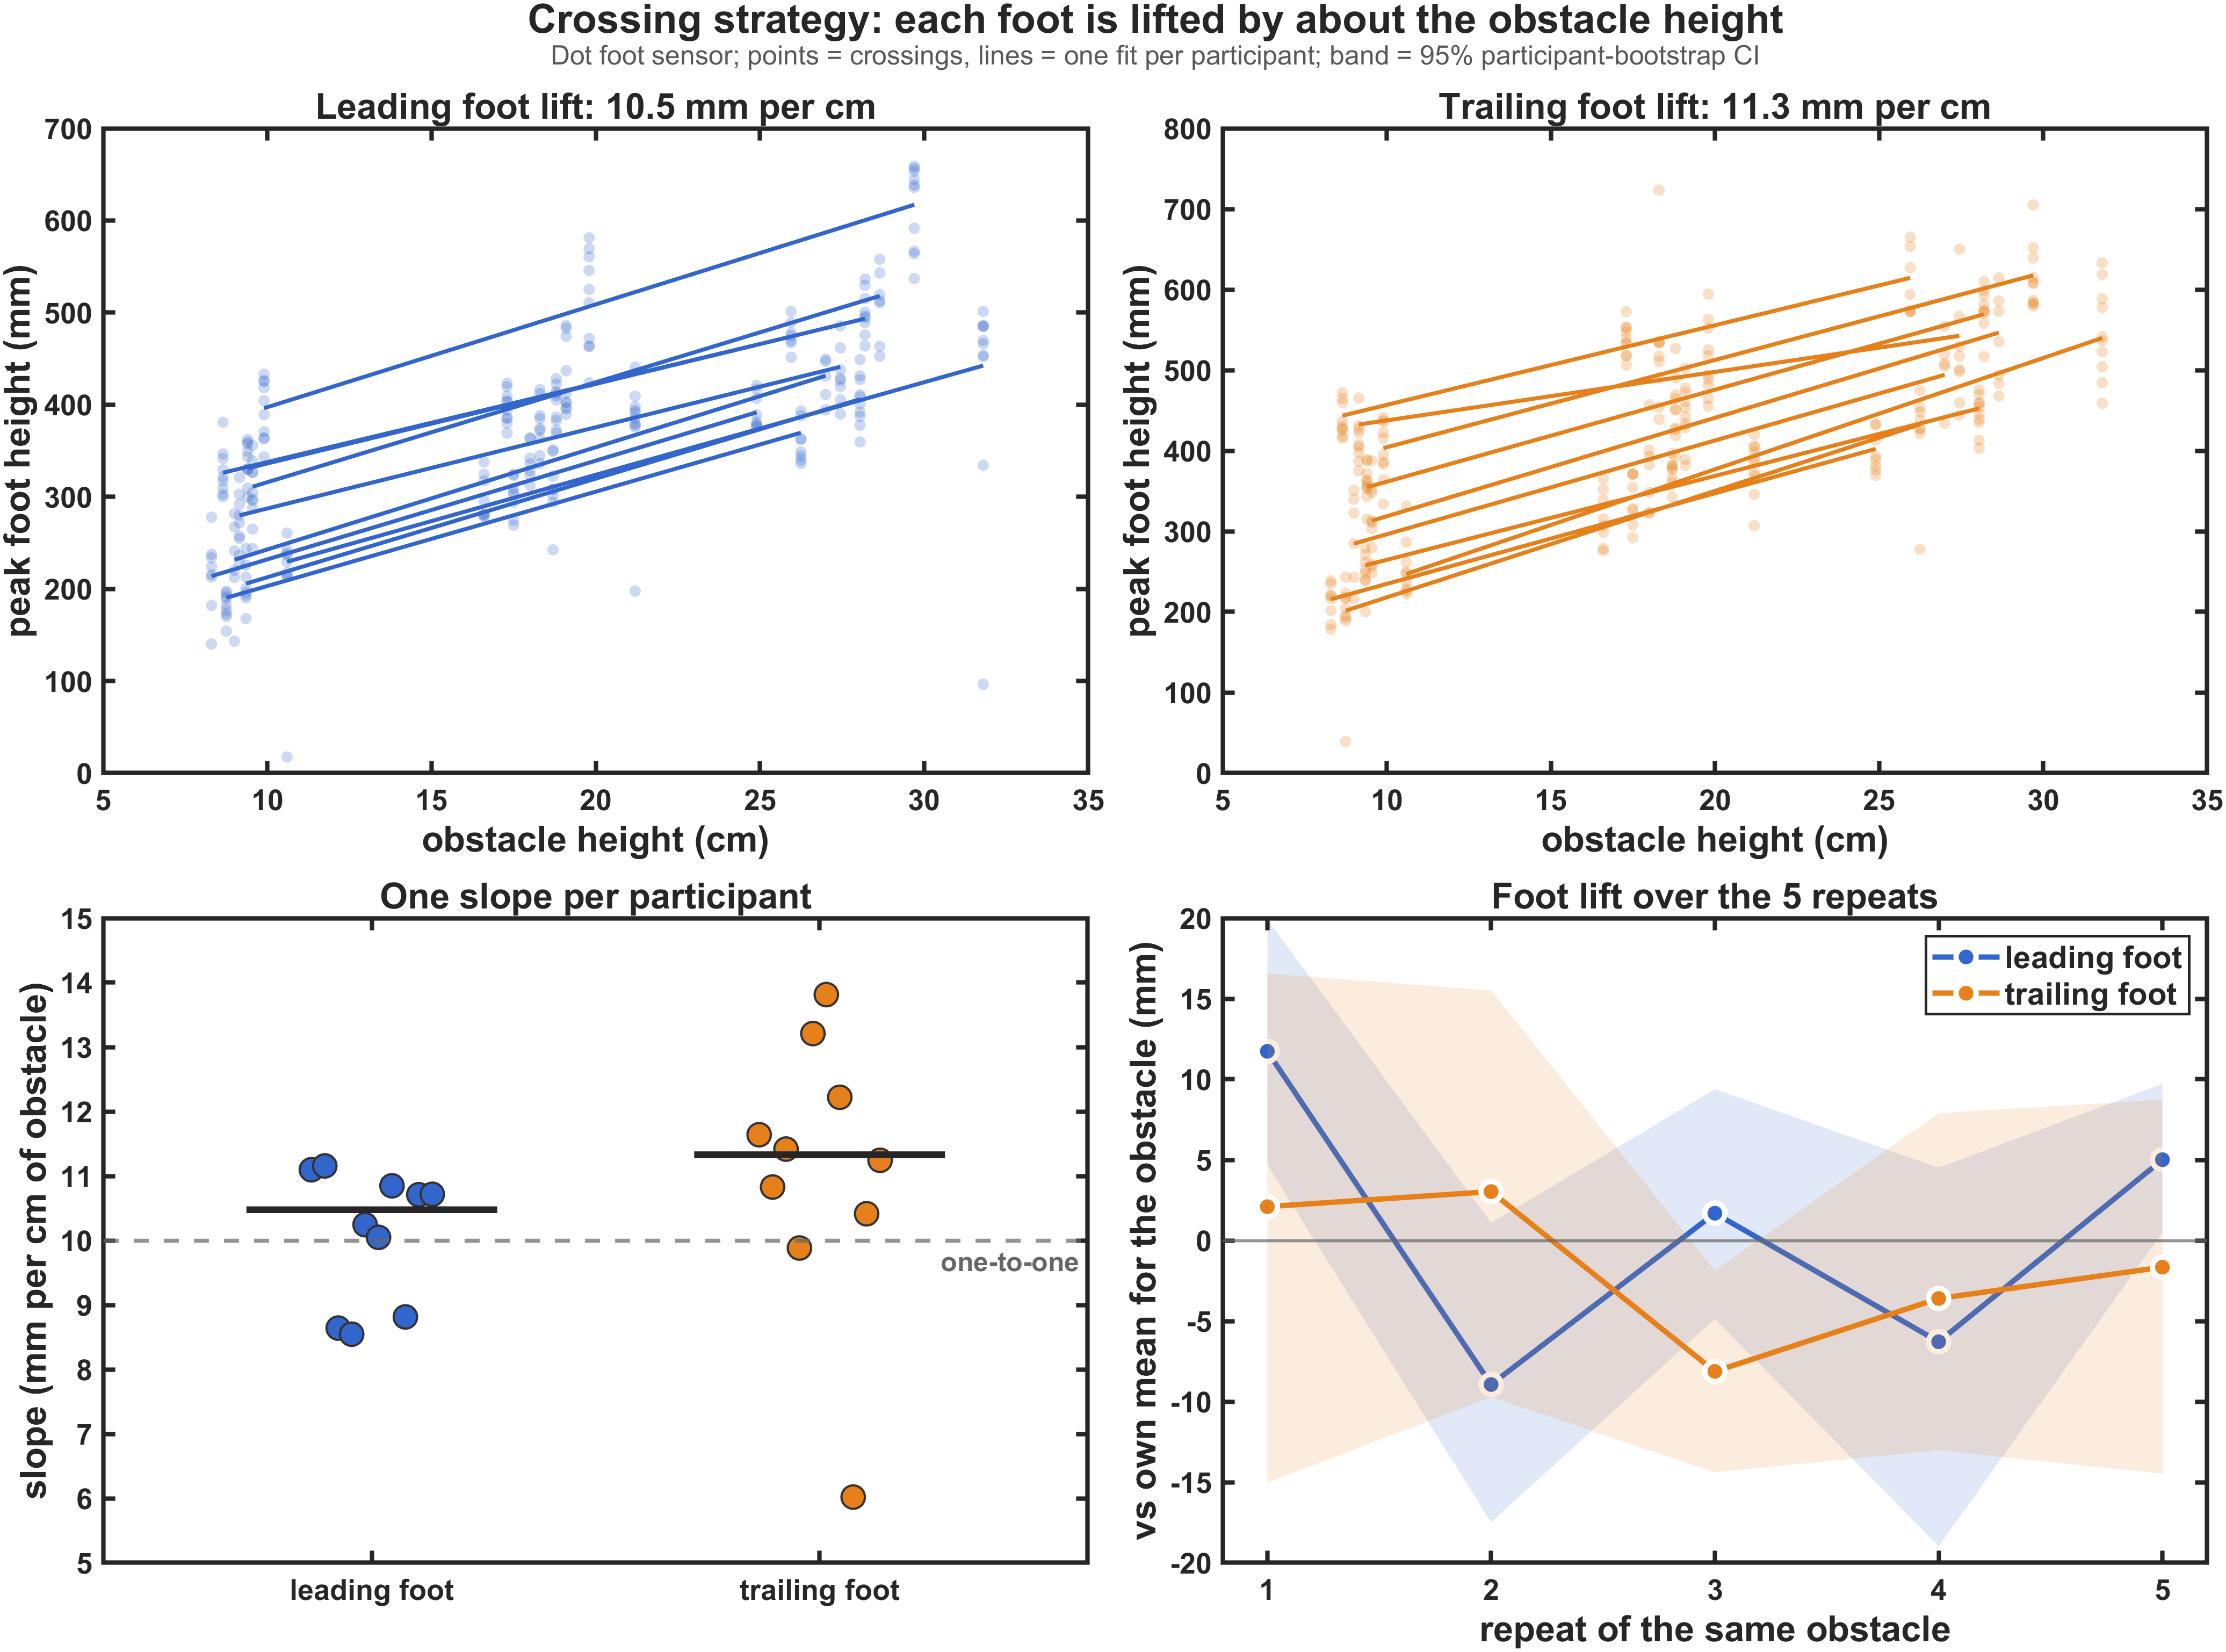
\includegraphics[width=\textwidth]{fig_story_strategy.png}
\caption{Crossing strategy. Top: foot lift measured by the Dot (foot-sensor rise above its stance height) against the nominal
obstacle height, leading (left) and trailing (right) foot; dots = crossings, one line per participant. Bottom left: the slope of each
participant (black bar = median; dashed = one-to-one, 10\,mm per cm). Bottom right: deviation of the foot lift from the participant
$\times$ obstacle mean over the five repeats of an obstacle (95\,\% CI). Source: \vn{crossing_ml_story.m}.}
\label{fig:strategy}
\end{figure}

\begin{table}[htbp]
\centering
\caption{Mixed-effects scaling with obstacle height: $y = \beta_0 + \beta_1 h + u_{0p} + u_{1p} h + \varepsilon$, slope $\beta_1$
per cm of obstacle (Satterthwaite CI and $p$).}
\label{tab:lme}
\begin{adjustbox}{max width=\textwidth}
{\footnotesize
\begin{tabular}{p{6cm}rrr}
\toprule
\textbf{variable} & \textbf{slope per cm} & \textbf{95\% CI} & \textbf{p} \\
\midrule
lead foot lift (Dot, mm) & +10.08 & +9.38 to +10.78 & $<$ 0.001 \\
trail foot lift (Dot, mm) & +11.12 & +9.66 to +12.59 & $<$ 0.001 \\
lead thigh flexion (deg) & +1.19 & +1.02 to +1.37 & $<$ 0.001 \\
trail shank backward tilt (deg) & $-$1.19 & $-$1.49 to $-$0.90 & $<$ 0.001 \\
lead min clearance (camera, mm) & $-$0.71 & $-$1.83 to +0.41 & 0.185 \\
trail min clearance (camera, mm) & $-$2.32 & $-$4.70 to +0.06 & 0.055 \\
\bottomrule
\end{tabular}
}
\end{adjustbox}

\end{table}

\paragraph{Adaptation over repeats.} The first crossing of a new obstacle has the highest leading-foot lift (+11.7\,mm above the
participant $\times$ obstacle mean, 95\,\% CI +4.7 to +19.9); later repeats scatter around the mean without a steady trend
(Figure~\ref{fig:strategy}, bottom right; Table~\ref{tab:adapt} in Appendix~\ref{app:extra}).

\subsubsection{Where and when the obstacle shows in the signals}

Figure~\ref{fig:map} shows, for every signal and every 2\,\% of the swing, the share of within-person variance explained by
height and by width ($\eta^2$). Table~\ref{tab:map} lists the peaks. Height is written most clearly in the trailing foot height
early in its swing ($\eta^2 = 0.76$ at 20\,\%), the trailing shank tilt at push-off (0.66 at 4\,\%), the leading foot height
around the apex (0.62 at 48\,\%) and the leading thigh tilt (0.47 at 60\,\%). The leading shank and leading foot tilt carry
little height information. Width never explains more than 8\,\% of any signal at any moment.

\begin{figure}[htbp]
\centering
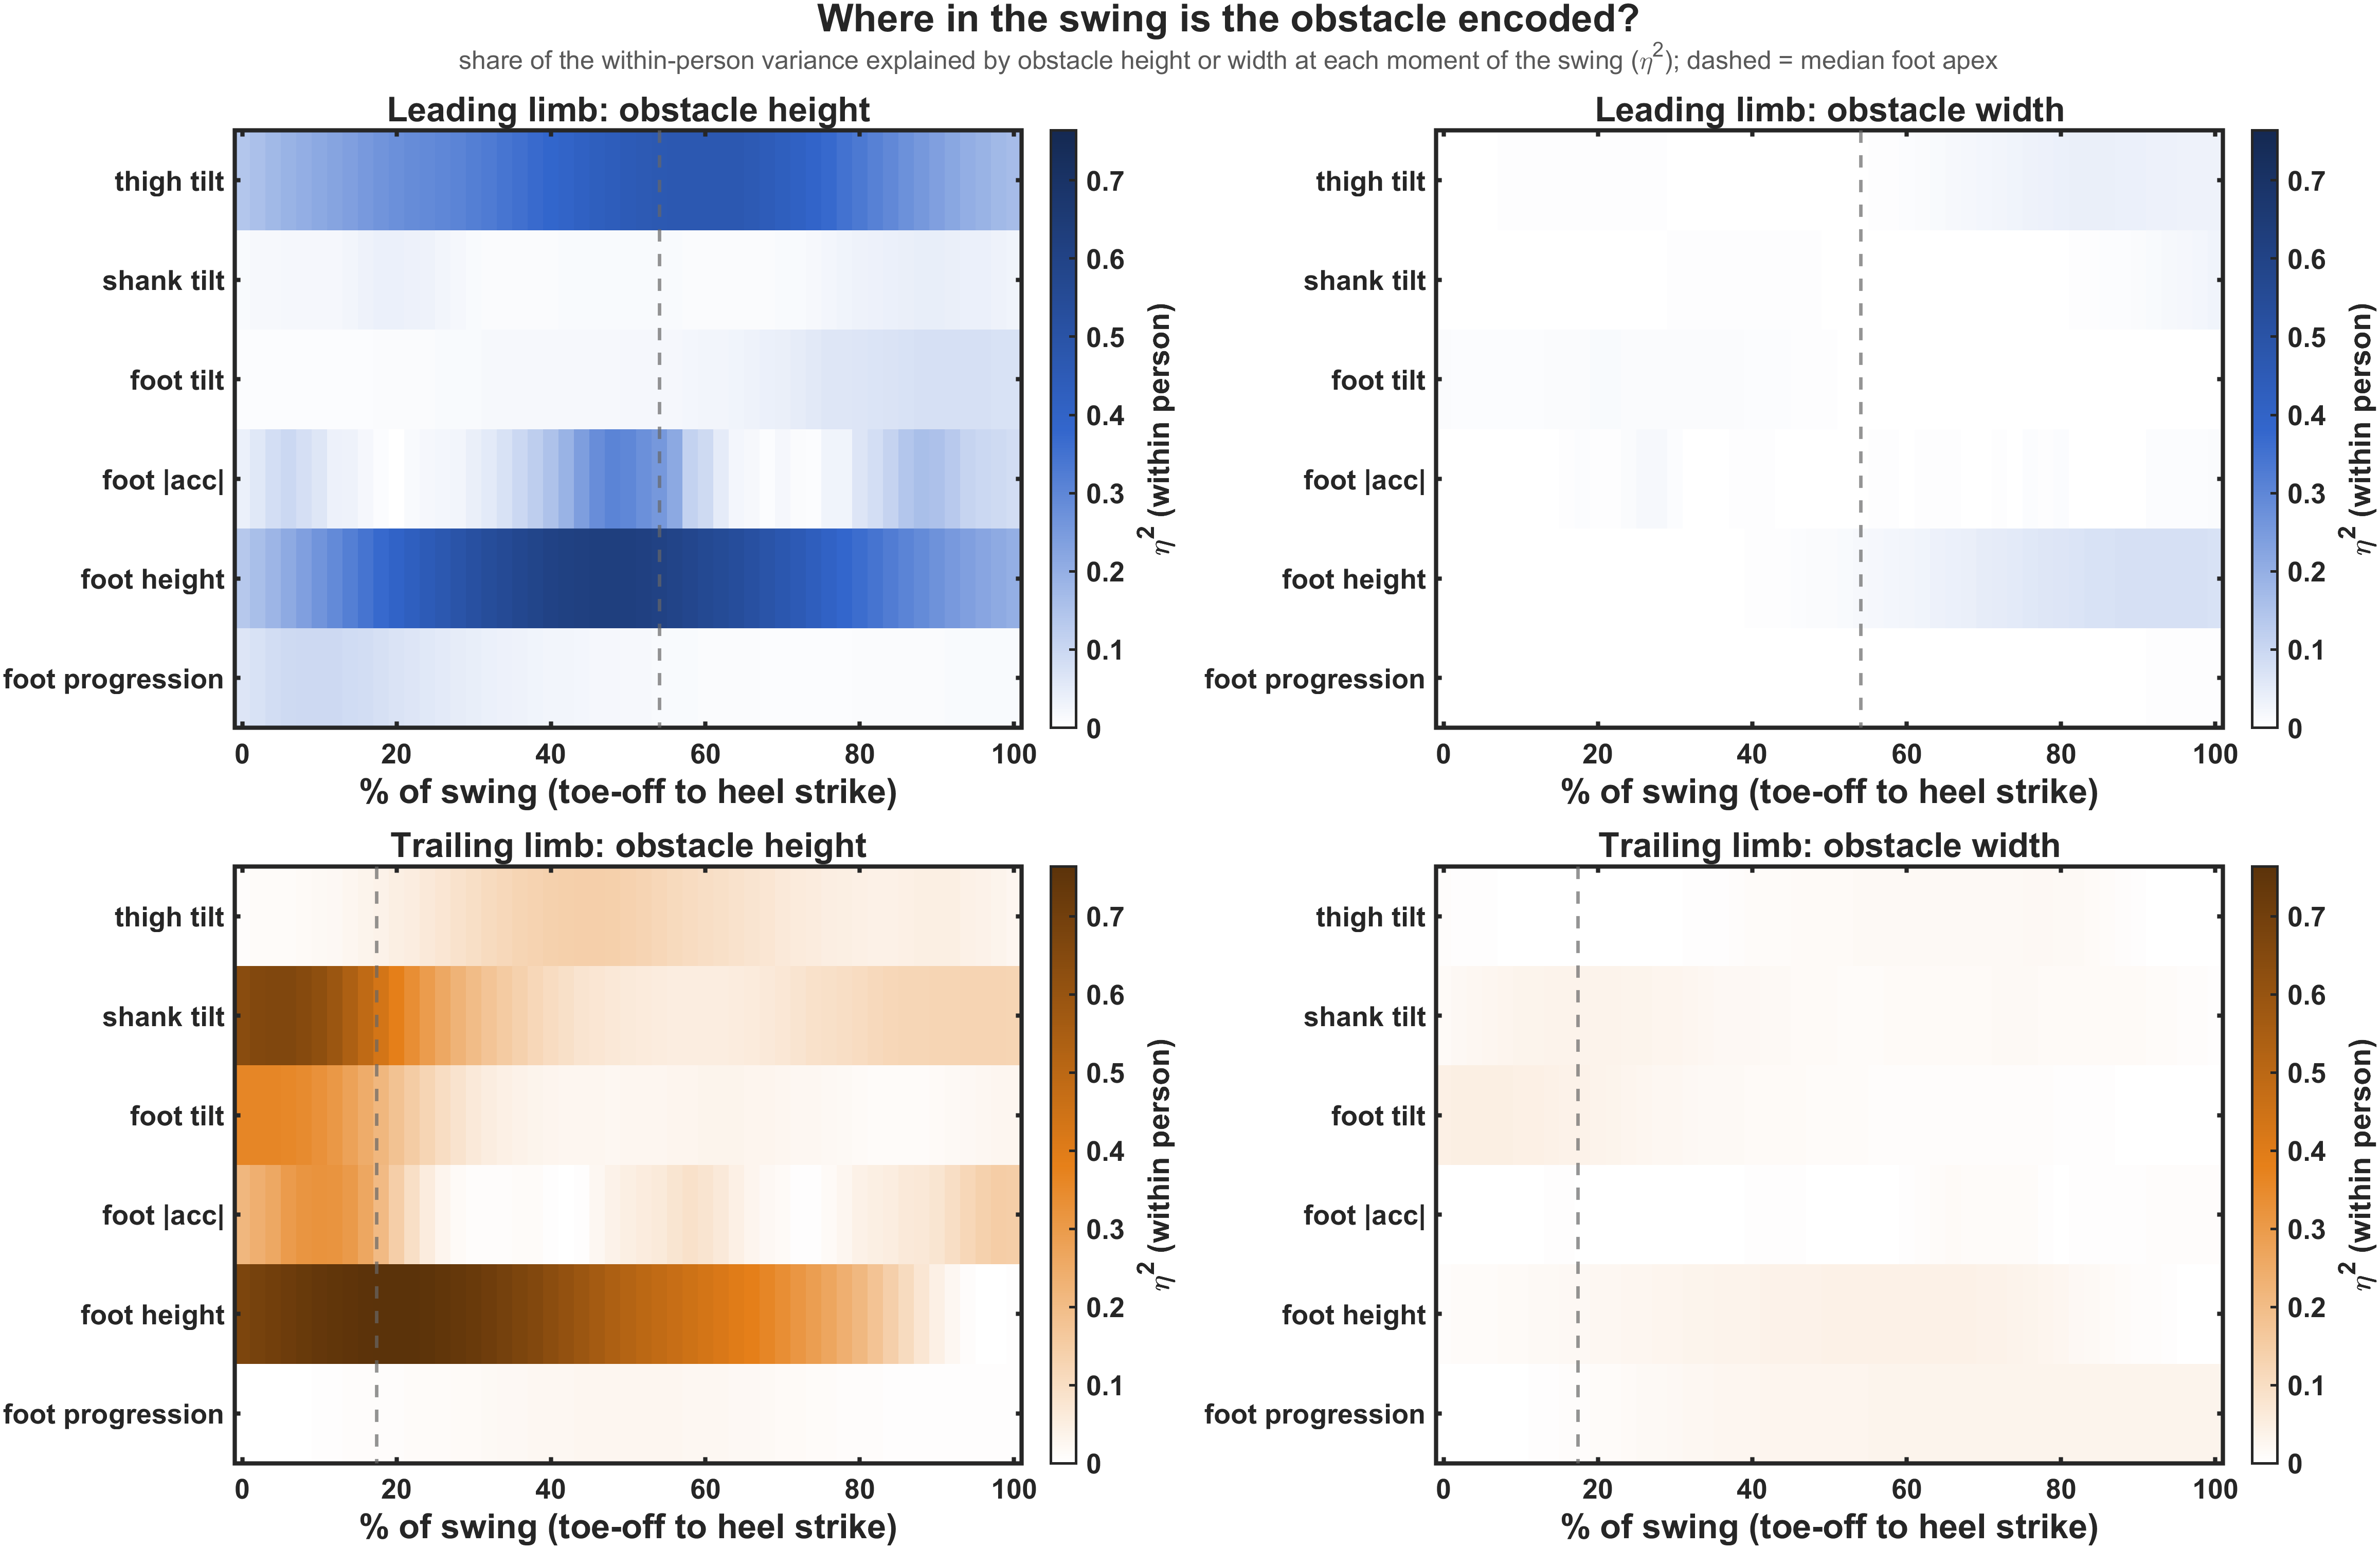
\includegraphics[width=\textwidth]{fig_story_map.png}
\caption{Within-person effect size $\eta^2$ of obstacle height (left) and width (right) at each moment of the swing, for the six
Dot swing signals of the leading (top, blue) and trailing (bottom, orange) limb, on the same scale. Dashed line = median foot apex.}
\label{fig:map}
\end{figure}

\begin{table}[htbp]
\centering
\caption{Peak $\eta^2$ of height and width per signal, and the share of variance explained by the participant (raw signals).}
\label{tab:map}
\begin{adjustbox}{max width=\textwidth}
{\footnotesize
\begin{tabular}{llrrrrr}
\toprule
\textbf{limb} & \textbf{signal} & \textbf{peak $\eta^2$ height} & \textbf{at \% swing} & \textbf{peak $\eta^2$ width} & \textbf{at \% swing} & \textbf{mean $\eta^2$ person (raw)} \\
\midrule
lead & thigh tilt & 0.47 & 60\% & 0.04 & 84\% & 0.40 \\
lead & shank tilt & 0.04 & 90\% & 0.03 & 100\% & 0.60 \\
lead & foot tilt & 0.08 & 90\% & 0.01 & 20\% & 0.46 \\
lead & foot |acc| & 0.31 & 48\% & 0.02 & 26\% & 0.32 \\
lead & foot height & 0.62 & 48\% & 0.08 & 92\% & 0.39 \\
lead & foot progression & 0.10 & 10\% & 0.01 & 100\% & 0.60 \\
trail & thigh tilt & 0.14 & 44\% & 0.02 & 76\% & 0.47 \\
trail & shank tilt & 0.66 & 4\% & 0.03 & 16\% & 0.40 \\
trail & foot tilt & 0.36 & 2\% & 0.05 & 6\% & 0.42 \\
trail & foot |acc| & 0.32 & 10\% & 0.01 & 66\% & 0.39 \\
trail & foot height & 0.76 & 20\% & 0.04 & 62\% & 0.48 \\
trail & foot progression & 0.03 & 50\% & 0.03 & 80\% & 0.71 \\
\bottomrule
\end{tabular}
}
\end{adjustbox}

\end{table}

\subsubsection{Every walker has a strong signature}

The participant explains far more variance than the obstacle: the median $\eta^2$ of the person over the 110 features is
0.42, that of height 0.02 (0.05 within person), and the person dominates in 99 of 110 features (Table~\ref{tab:person},
Figure~\ref{fig:person}). A logistic model identifies the participant from the features of a single crossing with 99.2\,\%
balanced accuracy (5-fold, chance 10\,\%). In a 2-D map of all crossings (t-SNE, Figure~\ref{fig:embed}) the raw features
cluster by participant (silhouette 0.48, by height $-0.04$); after person scaling they order by height (silhouette by height
0.26). This is the main reason why a model that has never seen the person is limited (Section~\ref{sec:res-height}).

\begin{table}[htbp]
\centering
\caption{Variance explained by the participant vs by the obstacle height (median over the 110 features).}
\label{tab:person}
\begin{adjustbox}{max width=\textwidth}
{\footnotesize
\begin{tabular}{p{5cm}rr}
\toprule
\textbf{} & \textbf{median over features} & \textbf{features where person $>$ height} \\
\midrule
$\eta^2$ person & 0.42 & 99 of 110 \\
$\eta^2$ height & 0.02 &  \\
$\eta^2$ height, within person & 0.05 &  \\
\bottomrule
\end{tabular}
}
\end{adjustbox}

\end{table}

\begin{figure}[htbp]
\centering
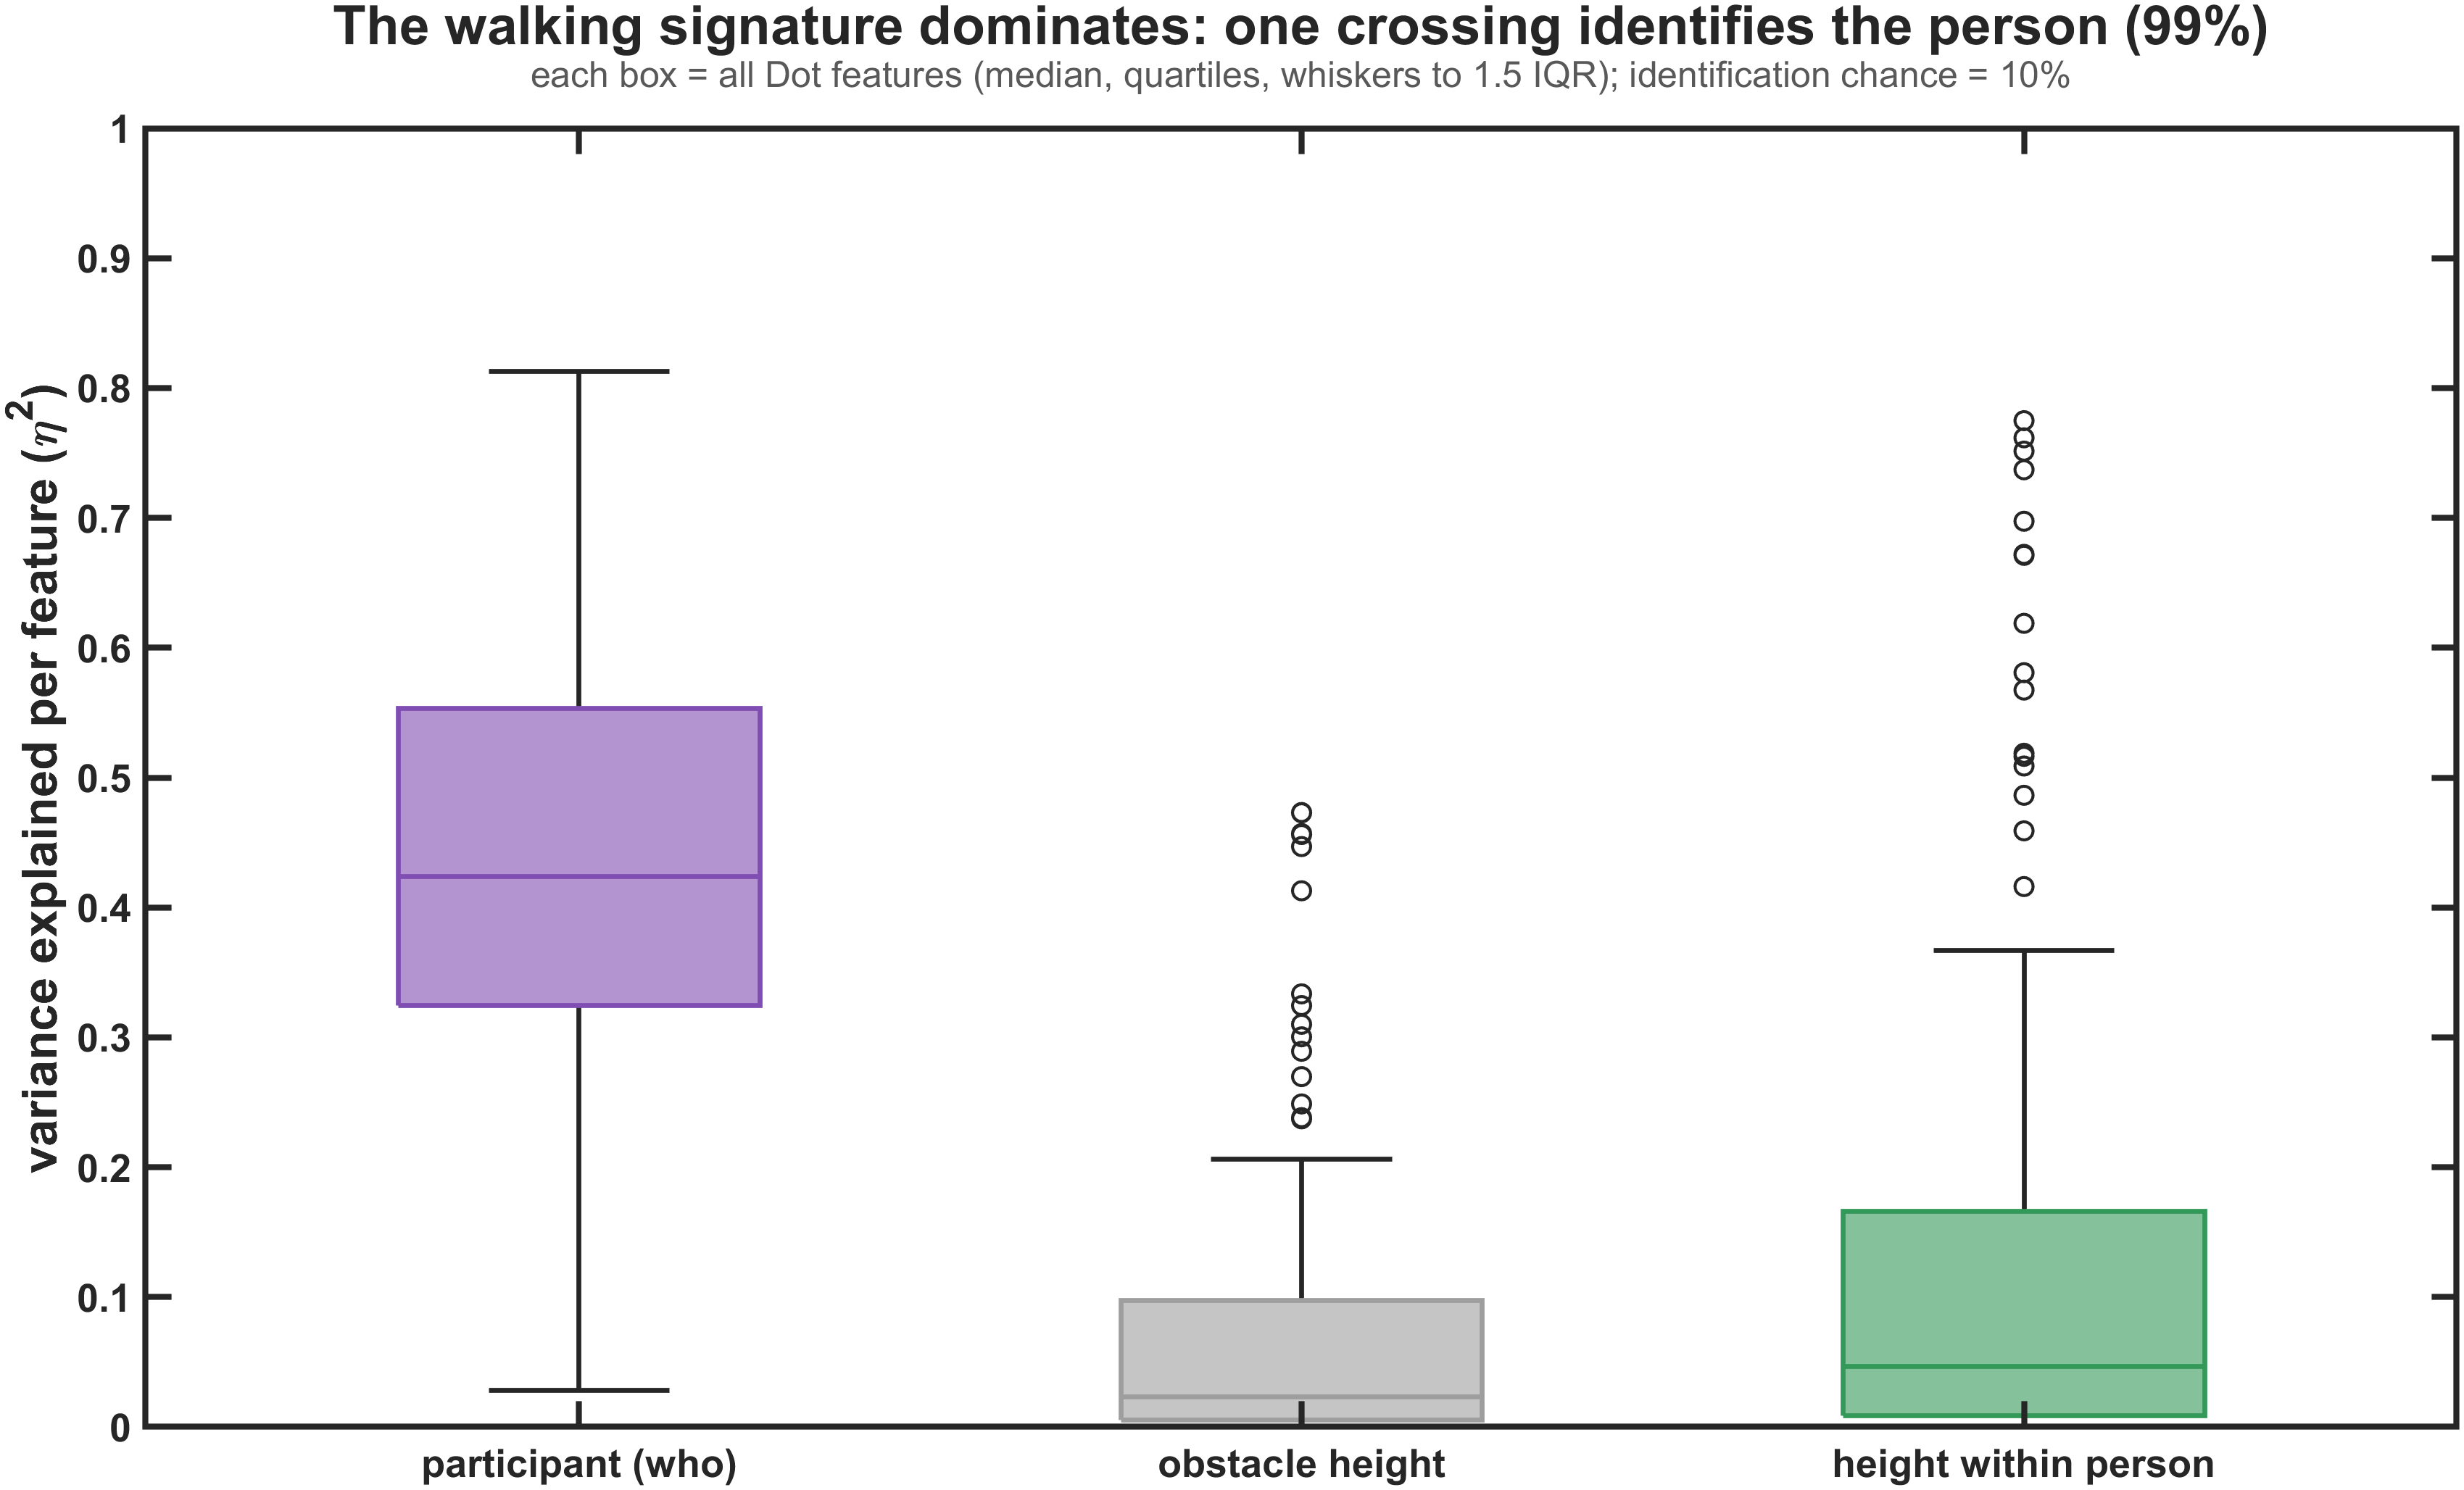
\includegraphics[width=0.78\textwidth]{fig_story_person.png}
\caption{Variance explained per feature by the participant (purple), by the obstacle height (grey), and by the height within each
participant (green); box = median and quartiles over the Dot features.}
\label{fig:person}
\end{figure}

\begin{figure}[htbp]
\centering
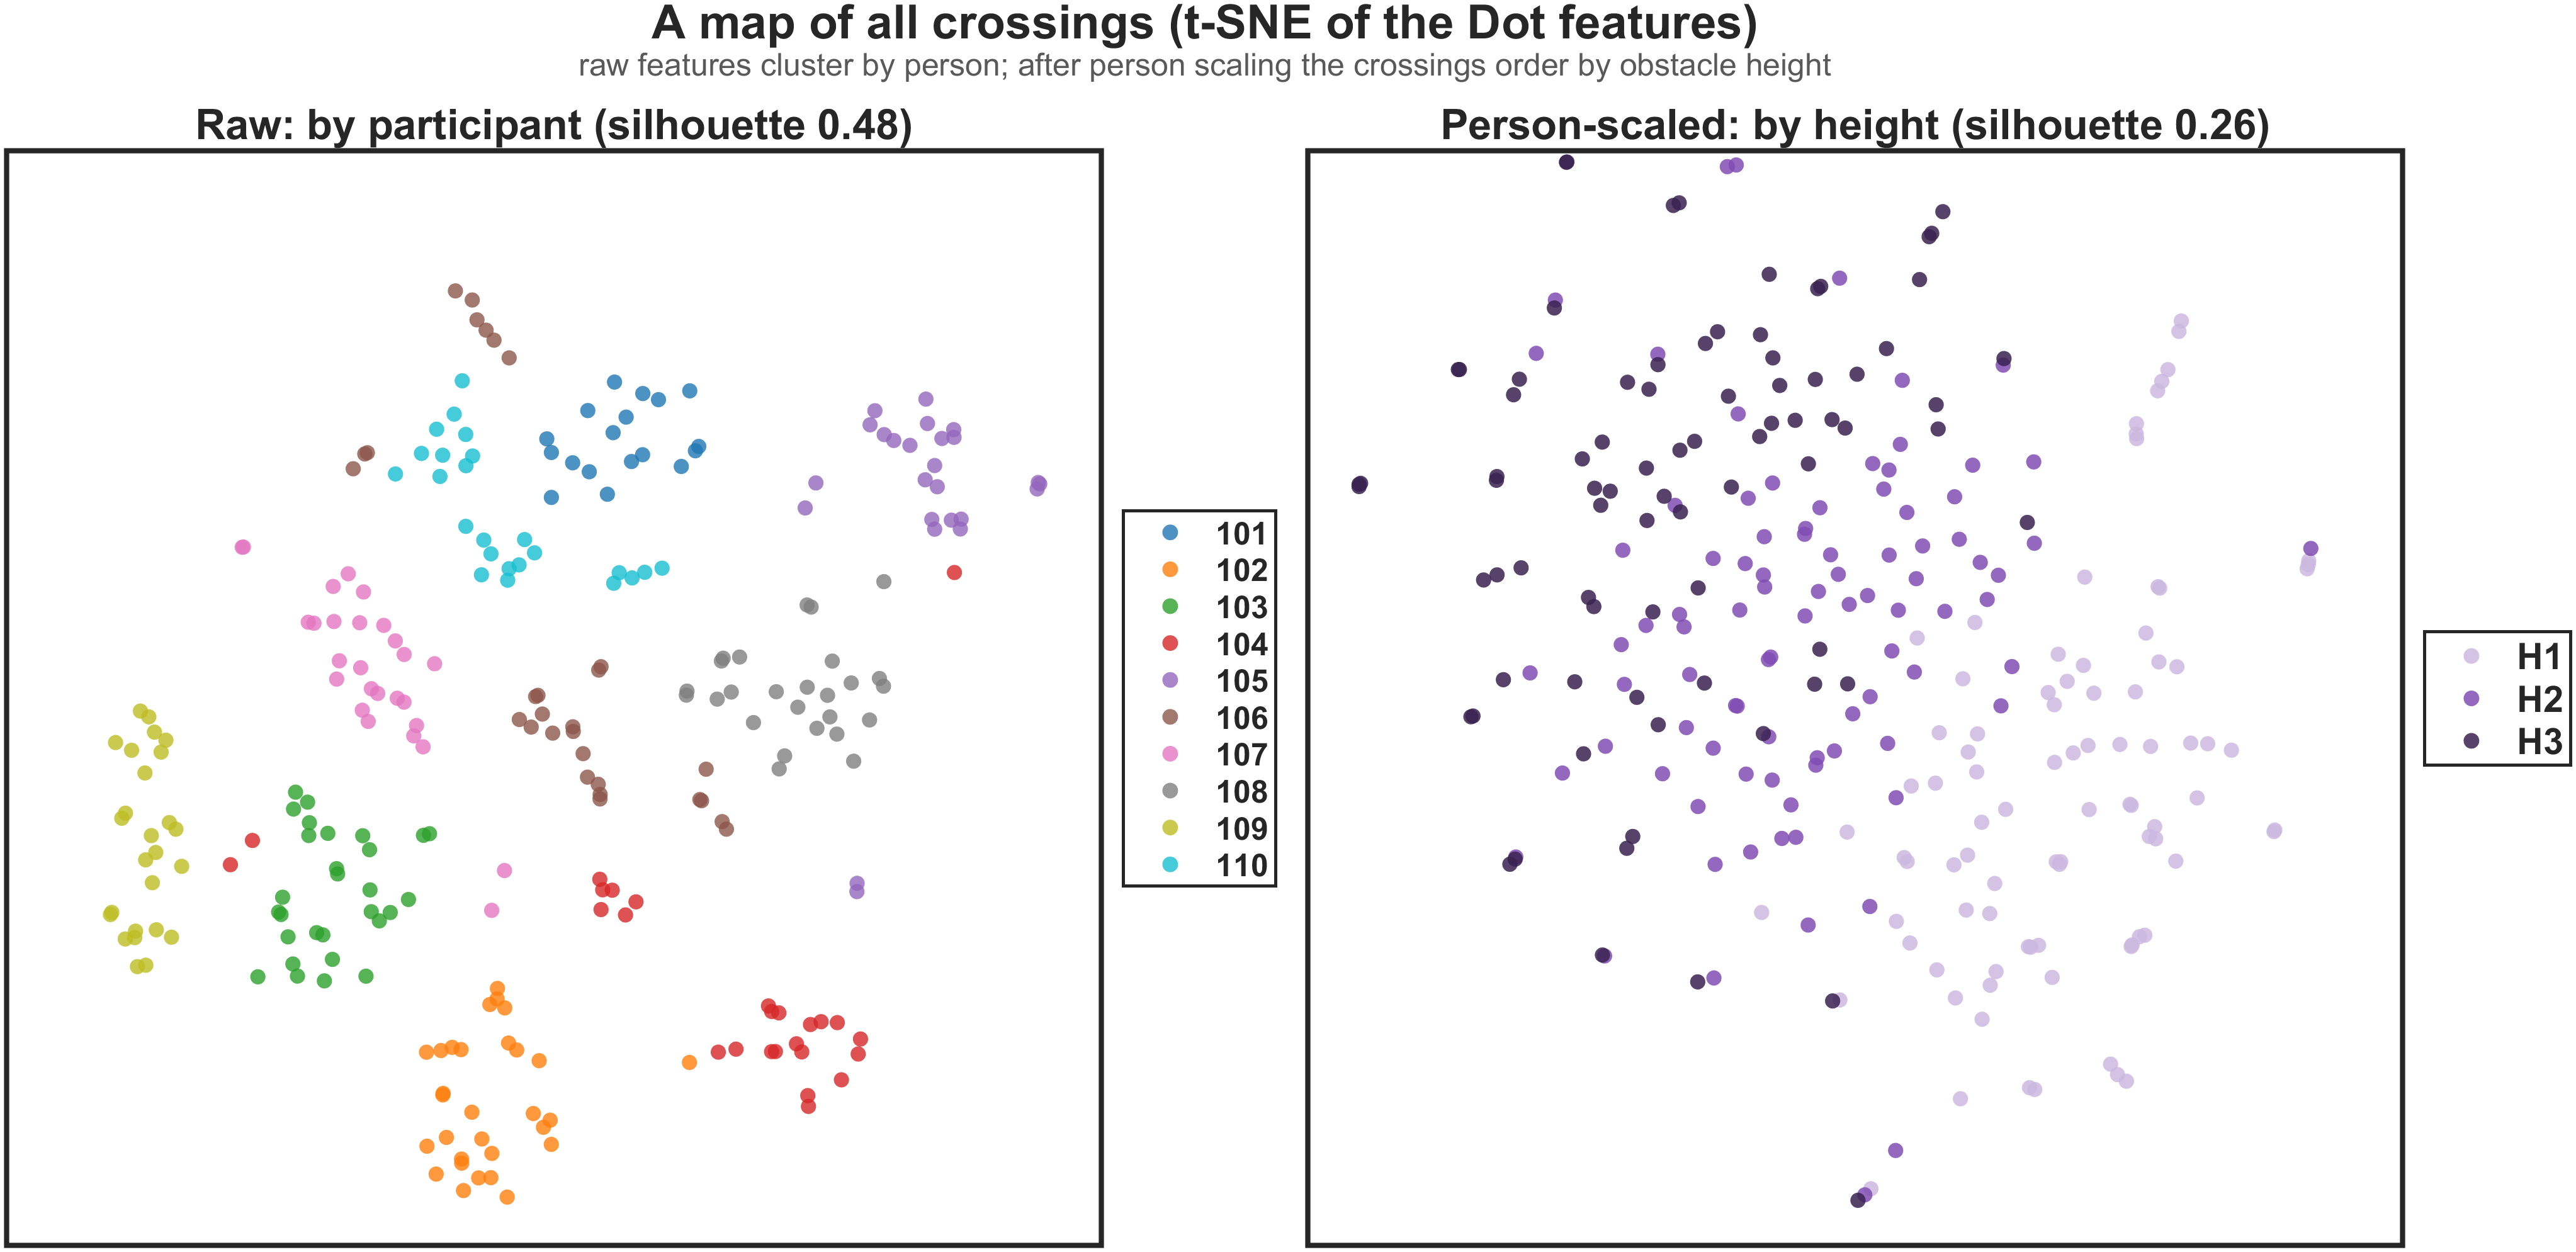
\includegraphics[width=\textwidth]{fig_story_embed.png}
\caption{t-SNE map of all crossings. Left: raw features coloured by participant. Right: person-scaled features coloured by
obstacle height (light to dark = H1 to H3). Silhouette (separation of the groups, $-1$ to 1) in the panel titles.}
\label{fig:embed}
\end{figure}

\subsubsection{The personal obstacle margin}

Per participant, the foot lift predicted by their own dose-response line at the cohort's mean obstacle height is their
``personal margin''. It differs between people by about two thirds of the step between neighbouring heights
(Table~\ref{tab:margin}: SD 64\,mm vs a 98\,mm step for the leading foot) and is barely predictable from the person's normal
walking ($r = 0.43$) or leg length ($r = 0.20$). An unseen person's margin therefore shifts every crossing toward a
neighbouring height, which caps generic models (Section~\ref{sec:res-height}).

\begin{table}[htbp]
\centering
\caption{Personal obstacle margin: spread across participants vs the step between heights.}
\label{tab:margin}
\begin{adjustbox}{max width=\textwidth}
{\footnotesize
\begin{tabular}{lrrrrr}
\toprule
\textbf{variable} & \textbf{between-person SD} & \textbf{step between heights} & \textbf{SD / step} & \textbf{r with level-walk value} & \textbf{r with leg length} \\
\midrule
lead foot lift & 64 mm & 98 mm & 0.66 & 0.43 & 0.20 \\
trail foot lift & 76 mm & 105 mm & 0.72 & $-$0.22 & 0.04 \\
\bottomrule
\end{tabular}
}
\end{adjustbox}

\end{table}

\subsubsection{The two legs}

The leading leg is not chosen by dominance: 45\,\% of the crossings were led with the dominant leg, and most participants
alternate (Table~\ref{tab:leads} in Appendix~\ref{app:extra}); the Dot recovers which leg leads in 100\,\% of the crossings
(Table~\ref{tab:leadtrail}). Within a crossing, once the shared obstacle effect is removed, the two legs vary independently
($\lvert r\rvert \leq 0.12$, Table~\ref{tab:coupling}): the leading leg tells how high the obstacle is, not whether the trailing
foot will under-lift on this crossing.

\begin{table}[htbp]
\centering
\caption{Coupling of the two legs: correlation of the crossing-to-crossing deviations from each participant $\times$ obstacle mean.}
\label{tab:coupling}
\begin{adjustbox}{max width=\textwidth}
{\footnotesize
\begin{tabular}{llr}
\toprule
\textbf{leading leg} & \textbf{trailing leg} & \textbf{r of the deviations} \\
\midrule
lead foot lift & trail foot lift & 0.11 \\
lead clearance (camera) & trail clearance (camera) & $-$0.12 \\
lead foot lift & trail clearance (camera) & $-$0.05 \\
lead thigh flexion & trail shank backward tilt & $-$0.07 \\
\bottomrule
\end{tabular}
}
\end{adjustbox}

\end{table}

\subsubsection{Does the camera confirm the scaling?}

The foot lift above is measured by the Dot foot sensor (on the top of the foot). The camera toe marker confirms the scaling but with a
smaller slope (Table~\ref{tab:validityslopes}): +8.8\,mm (leading) and +7.5\,mm (trailing) per cm of obstacle, against +10.1 and
+11.1\,mm for the sensor. The sensor rises more than the toe, especially on the trailing foot, which crosses heel-up. Crossing by
crossing (Table~\ref{tab:validityagree}), the sensor rise agrees well with the camera toe rise for the leading foot (bias +8\,mm,
$r = 0.82$, within person 0.90) and less for the trailing foot (bias +48\,mm, $r = 0.62$); the provisional rigid-body toe estimate
removes the trailing bias but not the scatter. Together with the flat clearance slope (Table~\ref{tab:lme}), people raise the toe by
slightly less than the obstacle height and accept a marginally smaller clearance for higher obstacles (not significant).

\begin{table}[htbp]
\centering
\caption{Foot lift per cm of obstacle measured by the camera toe marker and by the Dot (mixed model, 95\,\% CI).}
\label{tab:validityslopes}
\input{tables/validate_validity_slopes}
\end{table}

\begin{table}[htbp]
\centering
\caption{Agreement of the Dot foot lift with the camera toe rise, per crossing (Bland--Altman bias, SD and 95\,\% limits; correlation
overall and within participant).}
\label{tab:validityagree}
\input{tables/validate_validity_agree}
\end{table}

\subsubsection{No anticipation in the approach}

None of the variables available before the leading foot leaves the floor changes with obstacle height (Table~\ref{tab:anticipation}):
the two approach strides, the approach speed and the leading-foot stance all have slopes indistinguishable from zero and explain at
most 1\,\% of the within-person variance; the camera trailing-foot placement before the obstacle explains 4\,\%. The four IMU
approach variables classify the height at chance level (forest 41.6\,\%, logistic regression 30.8\,\%, permutation $p = 0.75$).
The adaptation to the obstacle height happens inside the crossing step itself, starting at the leading toe-off.

\begin{table}[htbp]
\centering
\caption{Anticipation: change per cm of obstacle of the variables before the crossing step (mixed model) and their within-person
$\eta^2$.}
\label{tab:anticipation}
\input{tables/validate_anticipation}
\end{table}


\subsection{Recognising obstacle height (Q2)}
\label{sec:res-height}

\subsubsection{Generic models versus person scaling}

Table~\ref{tab:limbs} is the central result. A \emph{generic} model (features referenced only to the person's level walk)
recognises the height of an unseen person's obstacle in 56--62\,\% of cases (chance 33\,\%). Scaling the features with the
person's own crossings (no labels) raises this to 80--90\,\%, the best being separate random forests for the leading and
trailing limb combined by soft vote: 90.0\,\% (85--95). The same holds for the six obstacles (29--30\,\% generic, 61\,\% with
person scaling; chance 17\,\%). Width stays close to chance with every setting (Section~\ref{sec:res-width}).

\begin{table}[htbp]
\centering
\caption{Height, width and the six obstacles from all Dot features of the leading limb, the trailing limb, or both (soft vote);
level-walk (generic) vs person (self) scaling; logistic regression vs random forest. Balanced accuracy (95\,\% CI).}
\label{tab:limbs}
\begin{adjustbox}{max width=\textwidth}
{\footnotesize
\begin{tabular}{lrllrrr}
\toprule
\textbf{target} & \textbf{chance} & \textbf{norm} & \textbf{model} & \textbf{lead} & \textbf{trail} & \textbf{fusion (lead + trail vote)} \\
\midrule
height & 33\% & level & logreg & 62.1\% (55--70) & 49.1\% (40--58) & 56.1\% (46--66) \\
height & 33\% & level & forest & 59.3\% (50--68) & 59.2\% (48--71) & 60.4\% (49--73) \\
height & 33\% & self & logreg & 79.6\% (73--86) & 78.0\% (67--87) & 80.8\% (74--87) \\
height & 33\% & self & forest & 87.6\% (82--92) & 86.1\% (79--92) & 90.0\% (85--95) \\
width & 50\% & level & logreg & 54.1\% (49--59) & 57.0\% (51--63) & 56.1\% (52--60) \\
width & 50\% & level & forest & 61.0\% (55--69) & 54.8\% (51--59) & 58.7\% (53--66) \\
width & 50\% & self & logreg & 64.6\% (63--67) & 58.5\% (53--65) & 64.3\% (59--69) \\
width & 50\% & self & forest & 61.9\% (58--66) & 56.9\% (53--61) & 59.2\% (54--64) \\
6 obstacles & 17\% & level & logreg & 28.6\% (22--35) & 27.5\% (24--32) & 29.1\% (23--35) \\
6 obstacles & 17\% & level & forest & 30.8\% (24--38) & 29.7\% (24--36) & 30.2\% (24--37) \\
6 obstacles & 17\% & self & logreg & 45.4\% (40--51) & 38.0\% (29--47) & 45.3\% (40--51) \\
6 obstacles & 17\% & self & forest & 49.8\% (42--58) & 57.9\% (51--66) & 61.2\% (54--69) \\
\bottomrule
\end{tabular}
}
\end{adjustbox}

\end{table}

Figure~\ref{fig:limbs} shows the same comparison for logistic regression, with two tasks the Dot solves almost perfectly: which
limb a swing belongs to, and whether a stride crosses an obstacle (Tables~\ref{tab:leadtrail} and \ref{tab:obslevel}). The generic
model's errors are almost all between neighbouring heights (Figure~\ref{fig:confusion}): H1 and H3 are confused in only 4 of 170
crossings, but the middle height H2 is recognised in only 39\,\% of cases (50\,\% with the leading limb alone). More training
participants would not close the gap (Figure~\ref{fig:learning}): with all features the generic model stays at 54--57\,\% from 2 to
9 training participants, and the leading-limb models gain at most 2 points from 6 to 9 participants. The limit of the generic
model is the difference between people, not the amount of data.

\begin{figure}[htbp]
\centering
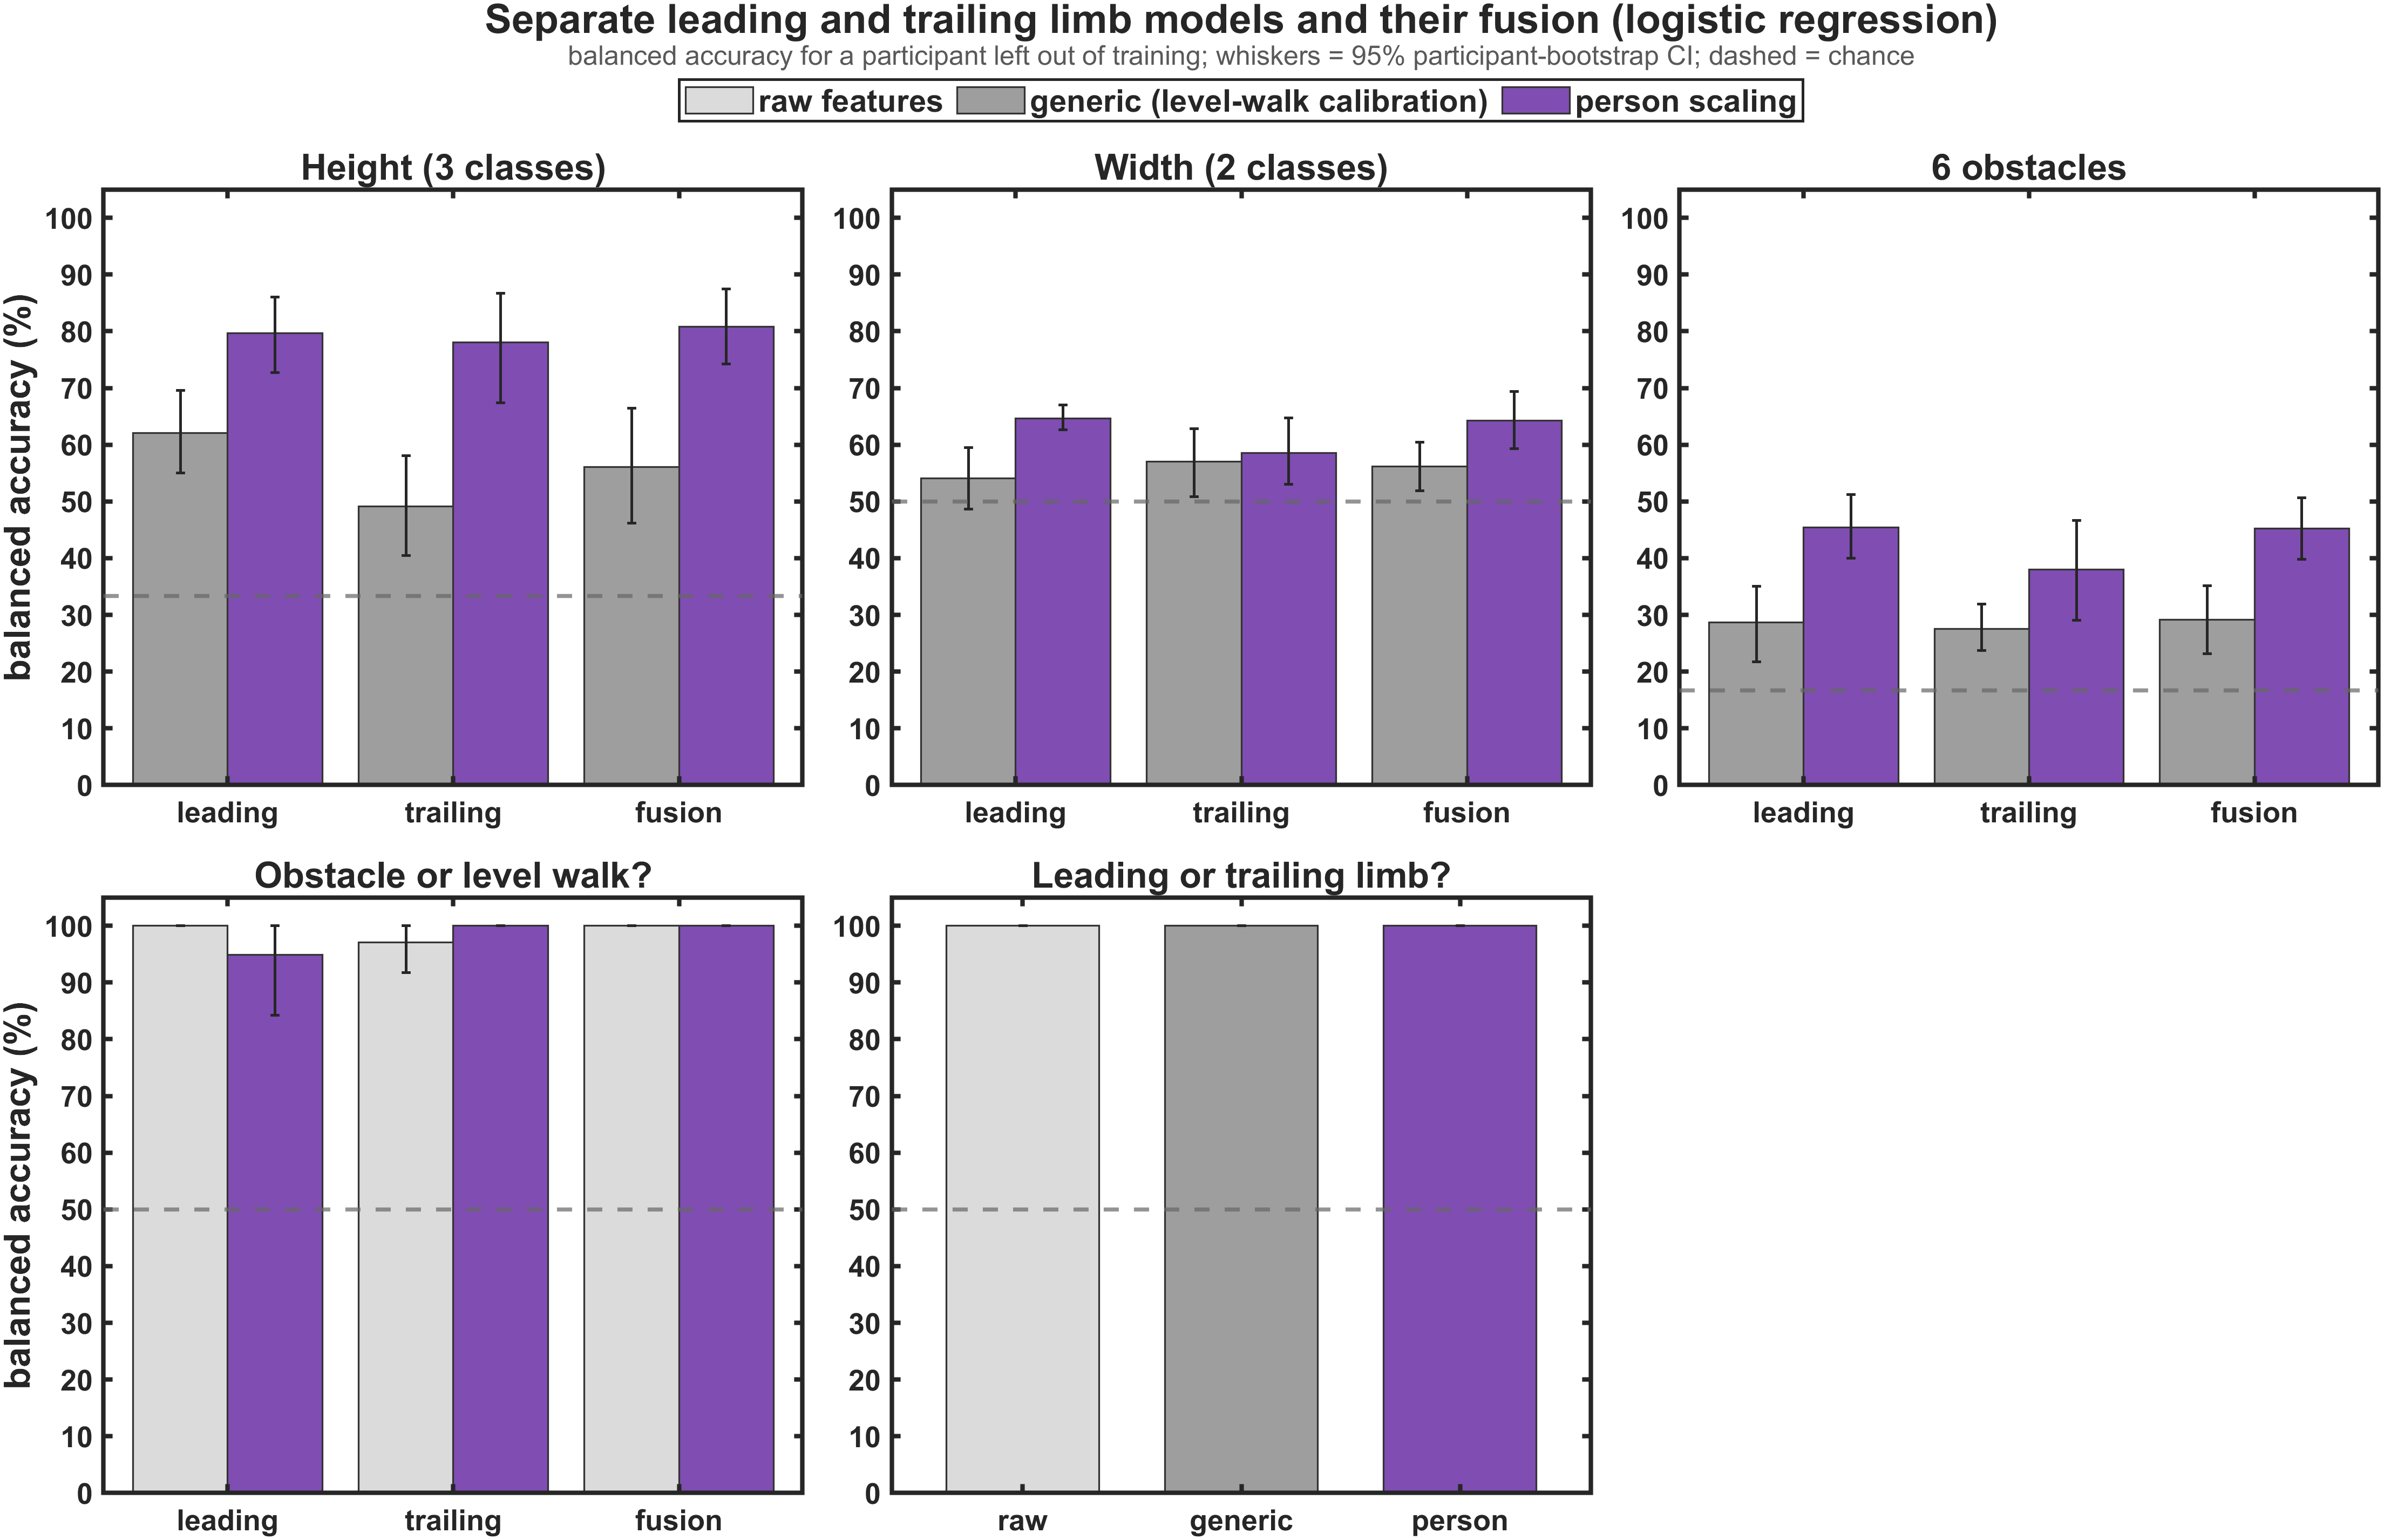
\includegraphics[width=\textwidth]{fig_limbs.png}
\caption{Separate models for the leading and the trailing limb and their soft-vote fusion (logistic regression): obstacle height, width
and the six obstacles, obstacle crossing versus level-walk stride, and which limb a swing belongs to. Bar colour = scaling: raw
features (light grey), generic level-walk calibration (grey), person scaling (purple). Whiskers = 95\,\% participant-bootstrap
CI; dashed = chance. Source: \vn{crossing_ml_matlab.m}, part 3.}
\label{fig:limbs}
\end{figure}

\begin{figure}[htbp]
\centering
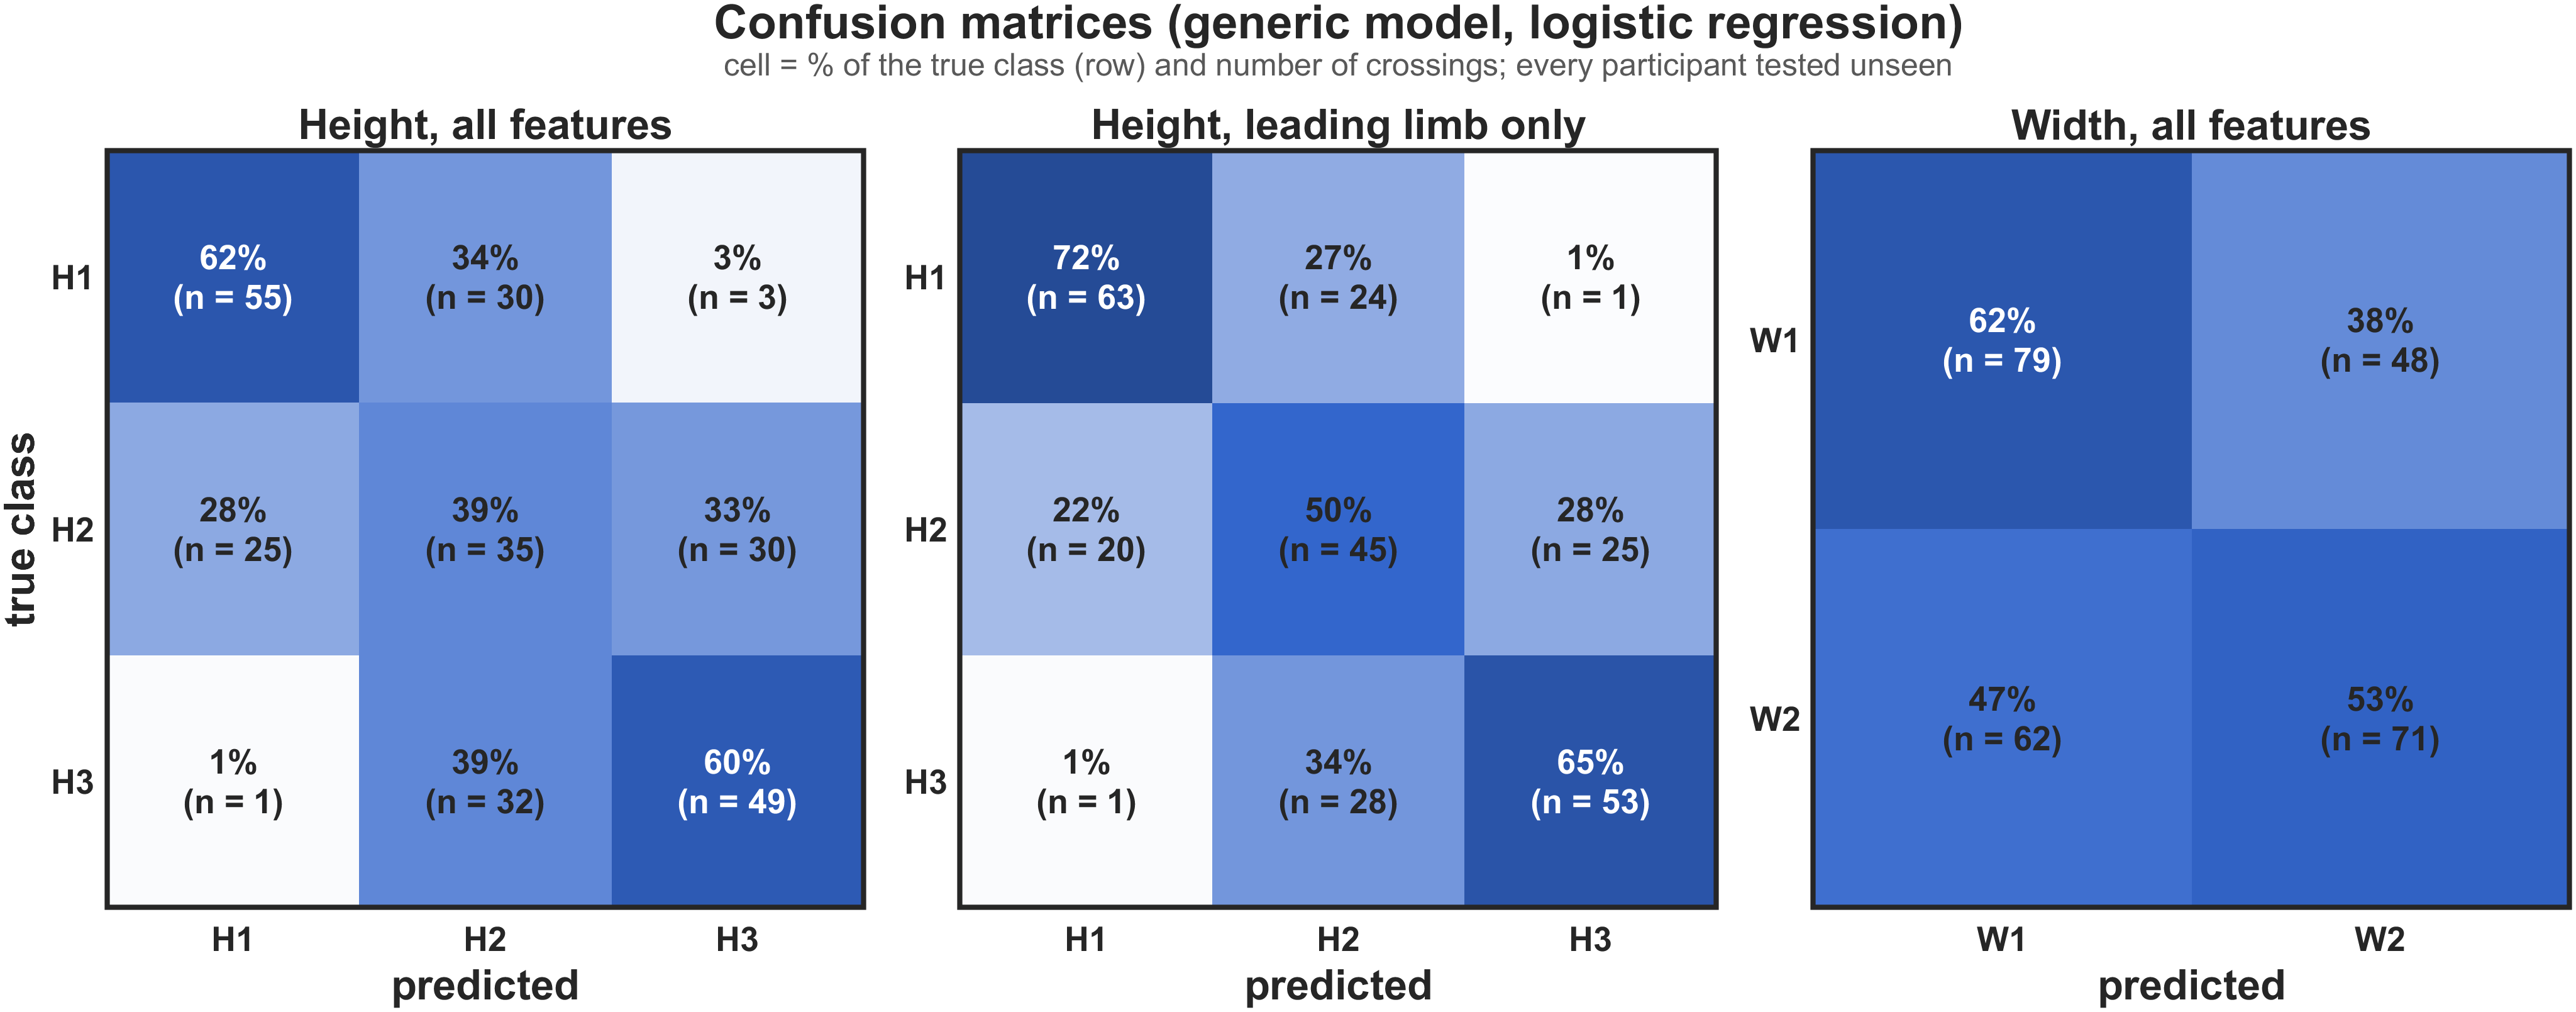
\includegraphics[width=\textwidth]{fig_confusion.png}
\caption{Confusion matrices of the generic model (logistic regression on level-walk-calibrated features): height from all features,
height from the leading limb only, and width. Cell = share of the true class (row) and number of crossings.}
\label{fig:confusion}
\end{figure}

\begin{figure}[htbp]
\centering
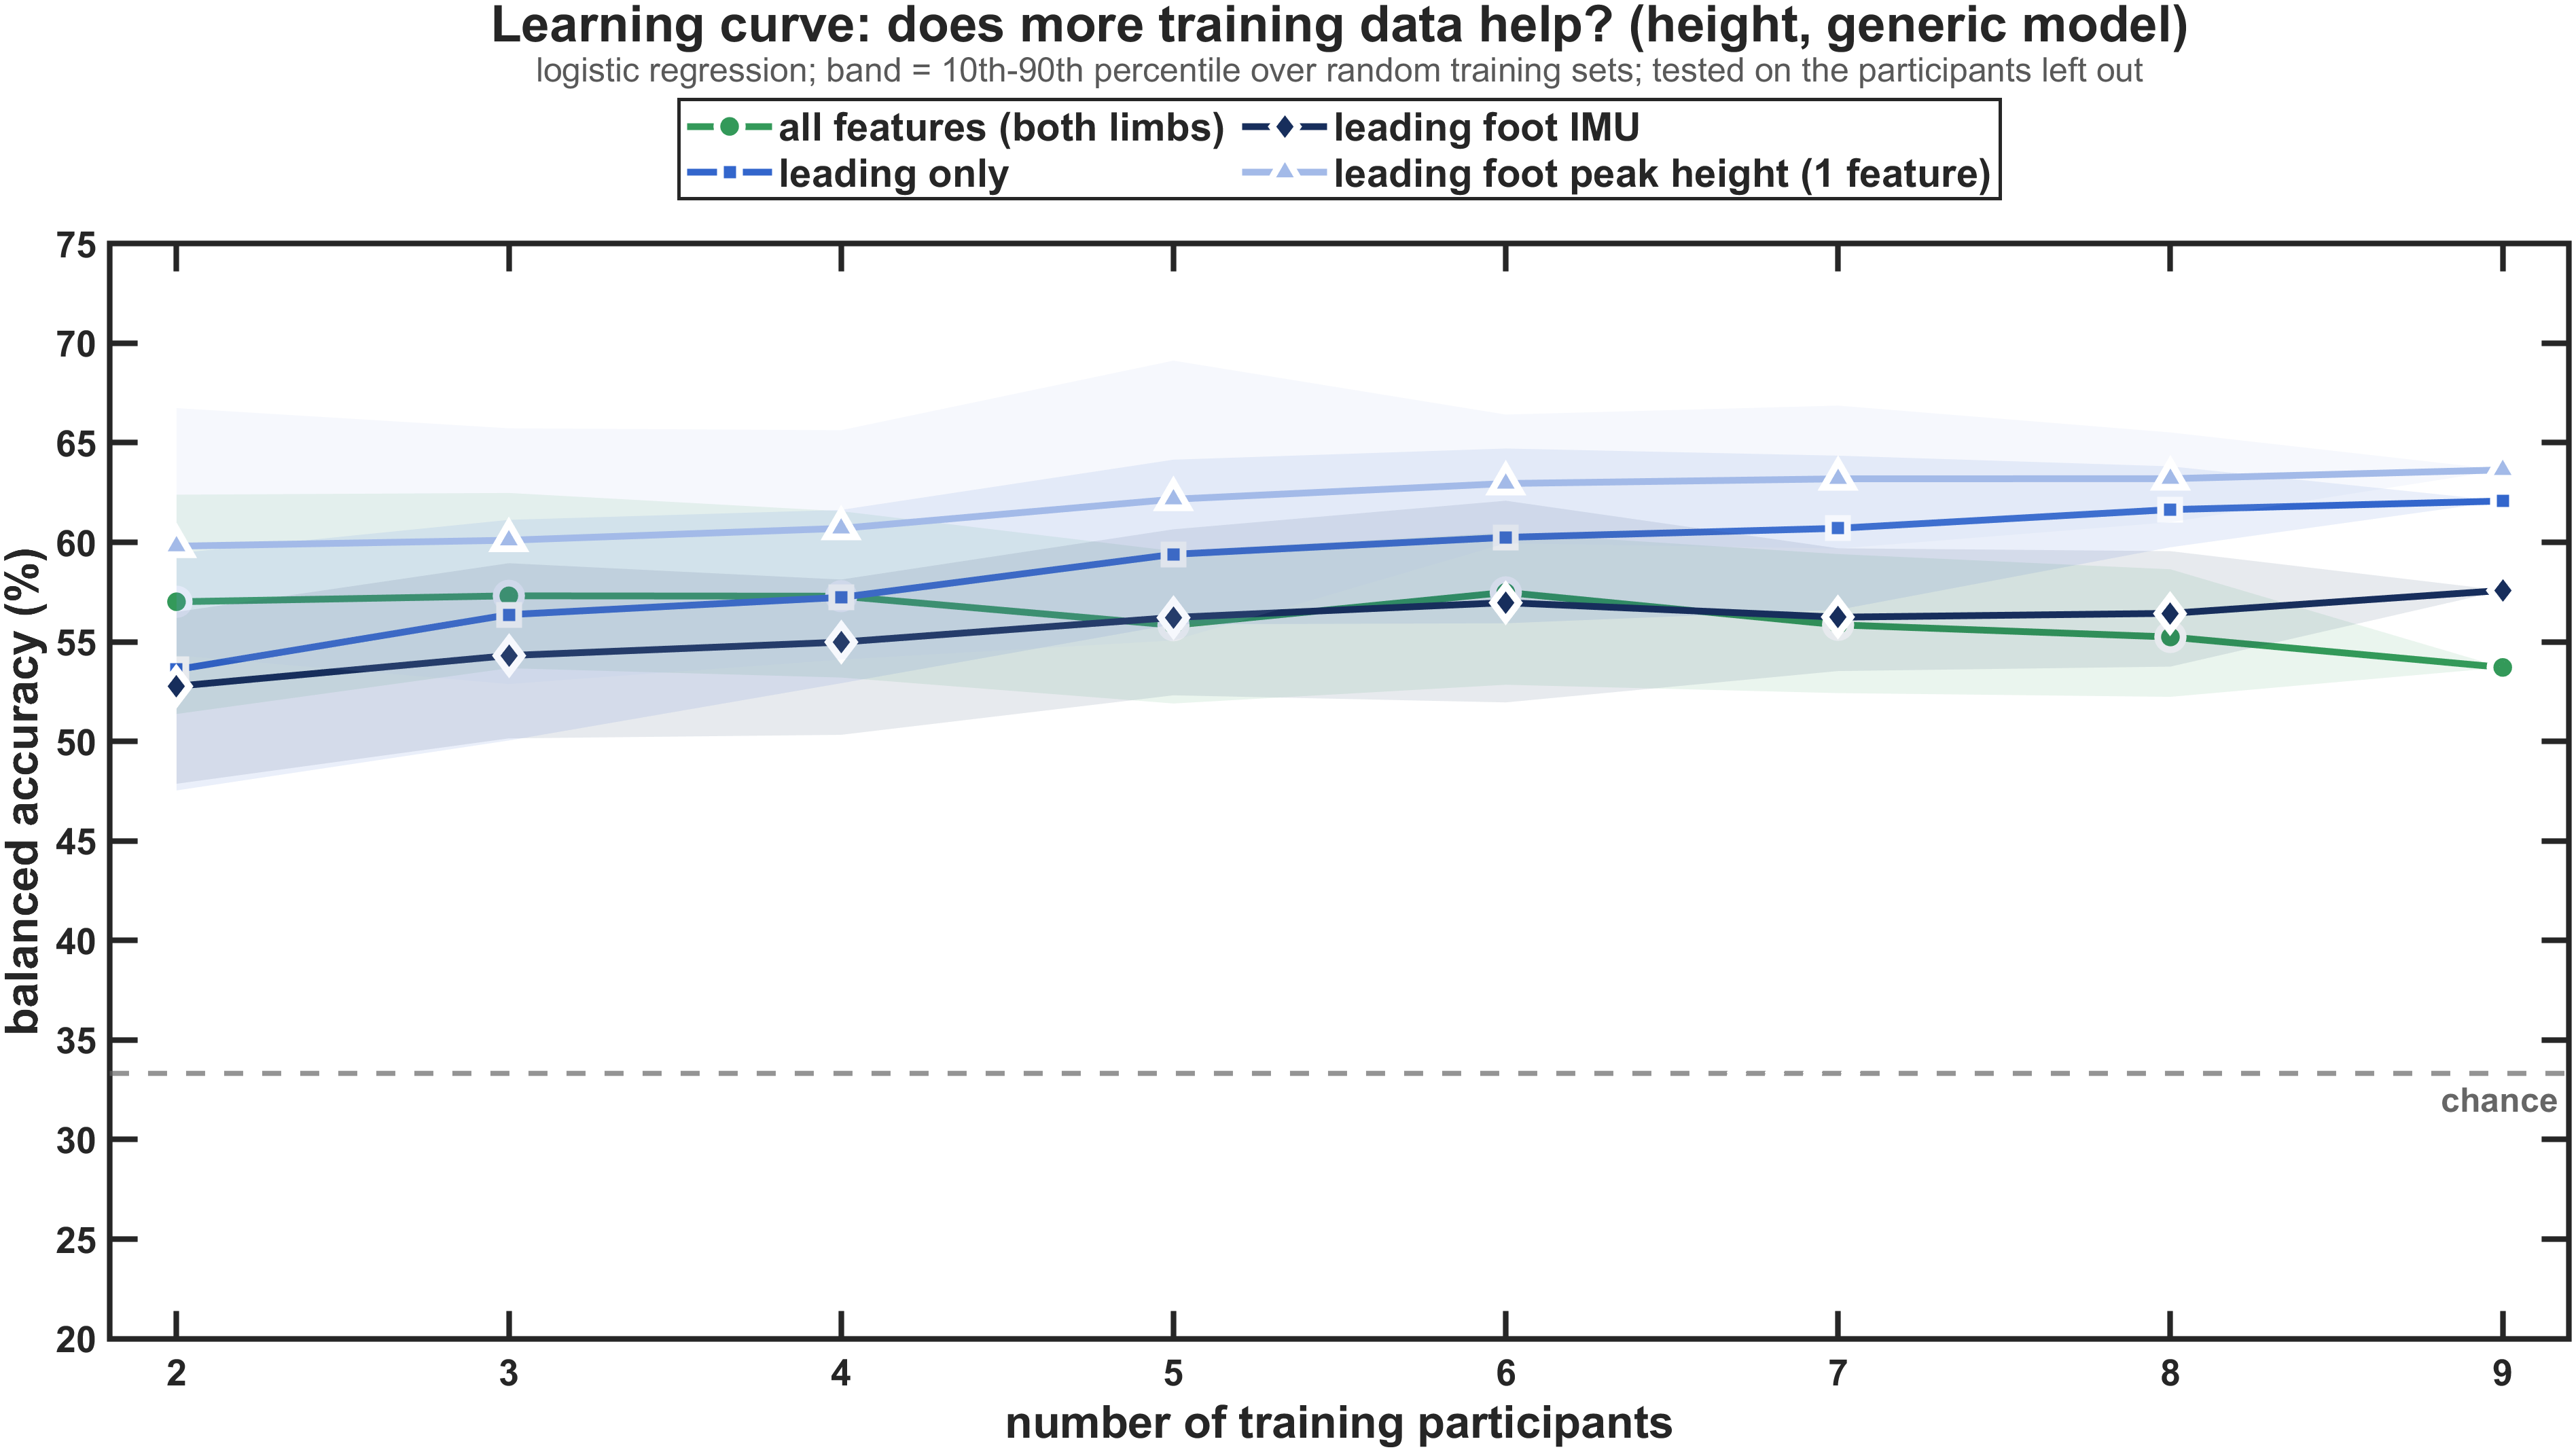
\includegraphics[width=\textwidth]{fig_learning_curve.png}
\caption{Learning curve of the generic model (height, logistic regression): each participant is predicted by a model trained on $n$
randomly chosen other participants (40 draws per $n$). Band = 10th--90th percentile over the draws; dashed = chance.}
\label{fig:learning}
\end{figure}

\subsubsection{Better inputs and models}

\paragraph{Clearance-shape features.} Thirteen numbers describing how long and how far the foot stays high
(Section~\ref{sec:features}) beat the 57 summary features in a generic model: 72.8\,\% vs 62.1\,\% with the leading limb and
logistic regression (permutation $p = 0.003$; Table~\ref{tab:inputs}). With person scaling they match the summary features
(89.7\,\% vs 90.4\,\% with the forest vote). The full swing curves do not add to the summary features.

\begin{table}[htbp]
\centering
\caption{Inputs compared: 57 summary features, 13 clearance-shape features, the swing curves and their combinations
(height; balanced accuracy, 95\,\% CI and the worst participant).}
\label{tab:inputs}
\begin{adjustbox}{max width=\textwidth}
{\footnotesize
\begin{tabular}{lrllrrr}
\toprule
\textbf{features} & \textbf{n feat (lead)} & \textbf{norm} & \textbf{model} & \textbf{lead} & \textbf{trail} & \textbf{fusion} \\
\midrule
summary & 57 & level & logreg & 62.1\% (55--70; worst 42\%) & 49.1\% (40--58; worst 27\%) & 56.1\% (46--66; worst 33\%) \\
summary & 57 & level & forest & 60.5\% (51--70; worst 31\%) & 58.8\% (47--71; worst 27\%) & 60.4\% (49--74; worst 27\%) \\
summary & 57 & self & logreg & 79.6\% (73--86; worst 57\%) & 78.0\% (67--87; worst 42\%) & 80.8\% (74--87; worst 65\%) \\
summary & 57 & self & forest & 88.4\% (83--93; worst 70\%) & 86.5\% (79--92; worst 62\%) & 90.4\% (85--95; worst 73\%) \\
shape & 13 & level & logreg & 72.8\% (65--80; worst 50\%) & 56.0\% (43--69; worst 27\%) & 63.7\% (51--77; worst 27\%) \\
shape & 13 & level & forest & 61.7\% (52--73; worst 38\%) & 53.6\% (42--66; worst 27\%) & 56.3\% (46--67; worst 27\%) \\
shape & 13 & self & logreg & 84.2\% (79--89; worst 72\%) & 75.1\% (68--81; worst 54\%) & 85.8\% (80--92; worst 65\%) \\
shape & 13 & self & forest & 86.1\% (82--91; worst 77\%) & 84.2\% (76--90; worst 58\%) & 89.7\% (86--93; worst 77\%) \\
curves & 66 & level & logreg & 60.6\% (52--68; worst 33\%) & 56.8\% (46--67; worst 27\%) & 57.9\% (47--70; worst 33\%) \\
curves & 66 & self & logreg & 75.0\% (68--81; worst 50\%) & 80.1\% (71--88; worst 50\%) & 82.3\% (75--90; worst 62\%) \\
summary + shape & 70 & level & logreg & 64.5\% (57--73; worst 42\%) & 50.6\% (41--60; worst 27\%) & 56.2\% (46--66; worst 33\%) \\
summary + shape & 70 & self & logreg & 83.4\% (77--89; worst 67\%) & 77.3\% (67--86; worst 42\%) & 83.0\% (77--89; worst 65\%) \\
summary + curves & 123 & level & logreg & 62.9\% (54--72; worst 37\%) & 53.1\% (42--64; worst 27\%) & 56.0\% (45--68; worst 33\%) \\
summary + curves & 123 & self & logreg & 80.8\% (77--85; worst 69\%) & 78.5\% (68--87; worst 42\%) & 82.3\% (75--89; worst 64\%) \\
\bottomrule
\end{tabular}
}
\end{adjustbox}

\end{table}

\paragraph{Models.} Random forests and boosted trees are the best single models with person scaling (88--90\,\%, soft vote);
the SVM and logistic regression are a few points lower (Table~\ref{tab:models}). A soft-vote ensemble of eight models reaches
91.5\,\%. The 1D convolutional network on the raw swing curves reaches 88.0\,\% with person scaling (Table~\ref{tab:cnn}) without
any hand-made feature, but no better than the forest on engineered features at this sample size.

\begin{table}[htbp]
\centering
\caption{Models compared with person scaling (height; balanced accuracy, 95\,\% CI, worst participant).}
\label{tab:models}
\begin{adjustbox}{max width=\textwidth}
{\footnotesize
\begin{tabular}{llrrr}
\toprule
\textbf{features} & \textbf{model} & \textbf{lead} & \textbf{trail} & \textbf{fusion} \\
\midrule
summary & logreg & 79.6\% (73--86; worst 57\%) & 78.0\% (67--87; worst 42\%) & 80.8\% (74--87; worst 65\%) \\
summary & forest & 88.4\% (83--93; worst 70\%) & 86.5\% (79--92; worst 62\%) & 90.4\% (85--95; worst 73\%) \\
summary & svm & 77.5\% (73--83; worst 67\%) & 80.0\% (72--87; worst 50\%) & 86.1\% (81--90; worst 69\%) \\
summary & boost & 87.3\% (81--92; worst 67\%) & 82.5\% (75--89; worst 54\%) & 88.4\% (83--94; worst 73\%) \\
shape & logreg & 84.2\% (79--89; worst 72\%) & 75.1\% (68--81; worst 54\%) & 85.8\% (80--92; worst 65\%) \\
shape & forest & 86.1\% (82--91; worst 77\%) & 84.2\% (76--90; worst 58\%) & 89.7\% (86--93; worst 77\%) \\
shape & svm & 81.5\% (76--87; worst 68\%) & 74.1\% (67--80; worst 54\%) & 86.9\% (82--92; worst 69\%) \\
shape & boost & 83.8\% (80--88; worst 73\%) & 86.2\% (81--90; worst 67\%) & 89.2\% (85--93; worst 80\%) \\
\bottomrule
\end{tabular}
}
\end{adjustbox}

\end{table}

\begin{table}[htbp]
\centering
\caption{1D convolutional network on the six swing curves of each limb (balanced accuracy).}
\label{tab:cnn}
\begin{adjustbox}{max width=\textwidth}
{\footnotesize
\begin{tabular}{llrrr}
\toprule
\textbf{normalization} & \textbf{target} & \textbf{lead} & \textbf{trail} & \textbf{fusion} \\
\midrule
level & height & 52.9\% & 53.1\% & 55.6\% \\
level & width & 52.3\% & 50.3\% & 50.7\% \\
self & height & 79.4\% & 82.6\% & 88.0\% \\
self & width & 50.0\% & 58.4\% & 56.5\% \\
\bottomrule
\end{tabular}
}
\end{adjustbox}

\end{table}

\paragraph{Honest selection.} Choosing the best setting by its test result is optimistic, so the choice was repeated inside each
training set (nested LOPO, Table~\ref{tab:nested}). Among generic settings the fair estimate is 69.4\,\% (58--80); among all 36
settings 91.5\,\% (86--97), with the person-scaled forest vote chosen in every fold (with summary + shape features in 9 of
10). Figure~\ref{fig:explore} summarises what each idea adds.

\begin{table}[htbp]
\centering
\caption{Nested selection of the setting (chosen inside each training set).}
\label{tab:nested}
\begin{adjustbox}{max width=\textwidth}
{\footnotesize
\begin{tabular}{lrp{3.6cm}p{6.6cm}}
\toprule
\textbf{candidate set} & \textbf{n settings} & \textbf{nested accuracy (95\% CI; worst participant)} & \textbf{settings chosen} \\
\midrule
generic & 18 & 69.4\% (58--80; worst 33\%) & shape, lead, logreg, level (9/10); summary, fusion, svm, level (1/10) \\
all & 36 & 91.5\% (86--97; worst 73\%) & summary + shape, fusion, forest, self (9/10); summary, fusion, forest, self (1/10) \\
\bottomrule
\end{tabular}
}
\end{adjustbox}

\end{table}

\begin{figure}[htbp]
\centering
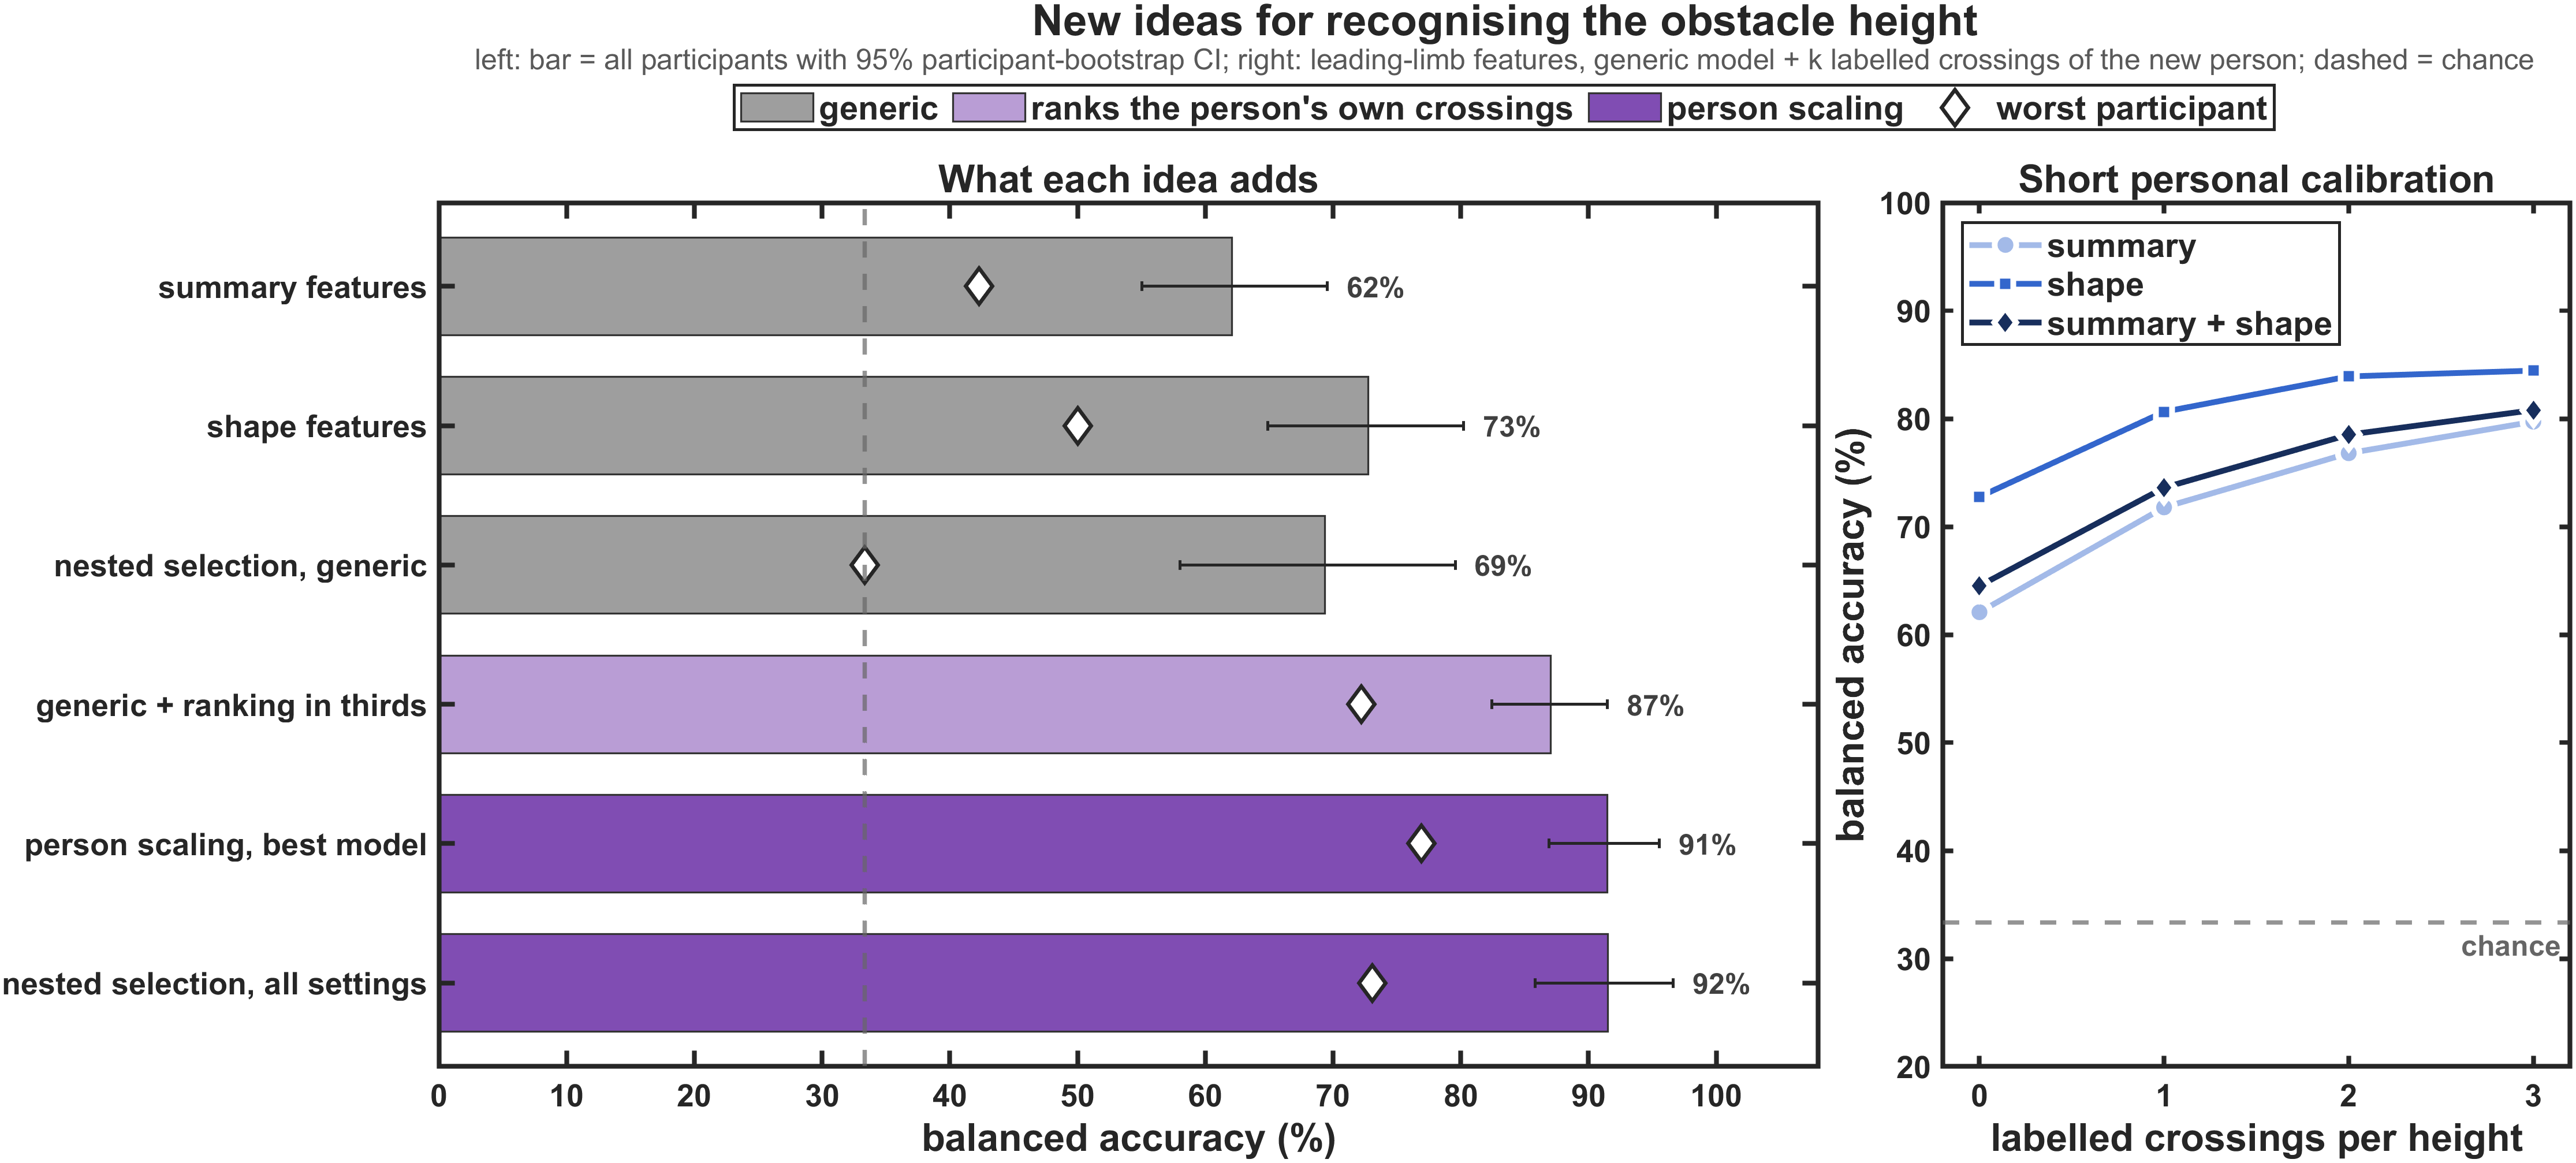
\includegraphics[width=\textwidth]{fig_explore.png}
\caption{Left: obstacle-height accuracy of the main ideas (bar = all participants with 95\,\% CI, diamond = worst participant;
grey = generic, light purple = ranks the person's own crossings, purple = person scaling). Right: generic model of the leading limb
plus a short personal calibration with $k$ labelled crossings per height.}
\label{fig:explore}
\end{figure}

\begin{table}[htbp]
\centering
\caption{What worked: summary of the model-improvement ideas (from \vn{ml_explore_matlab.md}).}
\label{tab:worked}
\begin{adjustbox}{max width=\textwidth}
{\footnotesize
\begin{tabular}{p{5.2cm}rrp{6.2cm}}
\toprule
\textbf{idea} & \textbf{before} & \textbf{after} & \textbf{comment} \\
\midrule
clearance-shape features, generic model (lead, level, logistic) & 62.1\% & \textbf{72.8\%} (p 0.003) & 13 features beat the 57 summary features without any person calibration \\
honest nested selection, generic settings only & 62.1\% & \textbf{69.4\%} (58--80) & best generic setting chosen fairly \\
+ ranking each person's crossings into thirds & 62.1\% & \textbf{87.0\%} & shape, fusion; assumes a mix of heights \\
1 labelled crossing per height from the new person & 71.8\% (summary) & \textbf{80.6\%} (shape) & 3 crossings of calibration \\
best single setting with self normalization & - & 90.4\% & summary, fusion, forest \\
best model / ensemble with self normalization & - & 91.5\% & ensemble (8 models), fusion, soft vote \\
honest nested selection, all settings & 89.3\% (Part 4.1) & \textbf{91.5\%} (86--97) & worst participant 73\% \\
self-training on the new person & 72.8\% (shape) & 54.0--67.1\% & did not help (the model reinforces its own errors) \\
width, best new idea & 64.3\% & 66.2\% & ratio + summary, fusion, logreg - width stays weak \\
\bottomrule
\end{tabular}
}
\end{adjustbox}

\end{table}

\subsubsection{Which segment and limb carries the information}

With person scaling (Table~\ref{tab:segments}), the foot is the best site: the foot angles alone give 88.1\,\% and the foot
trajectory 89.2\,\%. The thigh carries the leading limb's information (77.4\,\% leading, 44.2\,\% trailing) and the shank the
trailing limb's (78.2\,\% trailing, 49.8\,\% leading), matching where height appears in the signals (Figure~\ref{fig:map}). The
foot acceleration alone is weak.

Without person scaling (Figure~\ref{fig:featuresets}) every feature set predicts the height above its permutation null
($p \leq 0.037$), but the best set, the leading foot angles, reaches only 66.5\,\%. The limb pattern is the same as with person
scaling: the thigh and the foot angles carry more in the leading limb, the shank in the trailing limb. Width stays at 46--59\,\%,
around its null.

\begin{figure}[htbp]
\centering
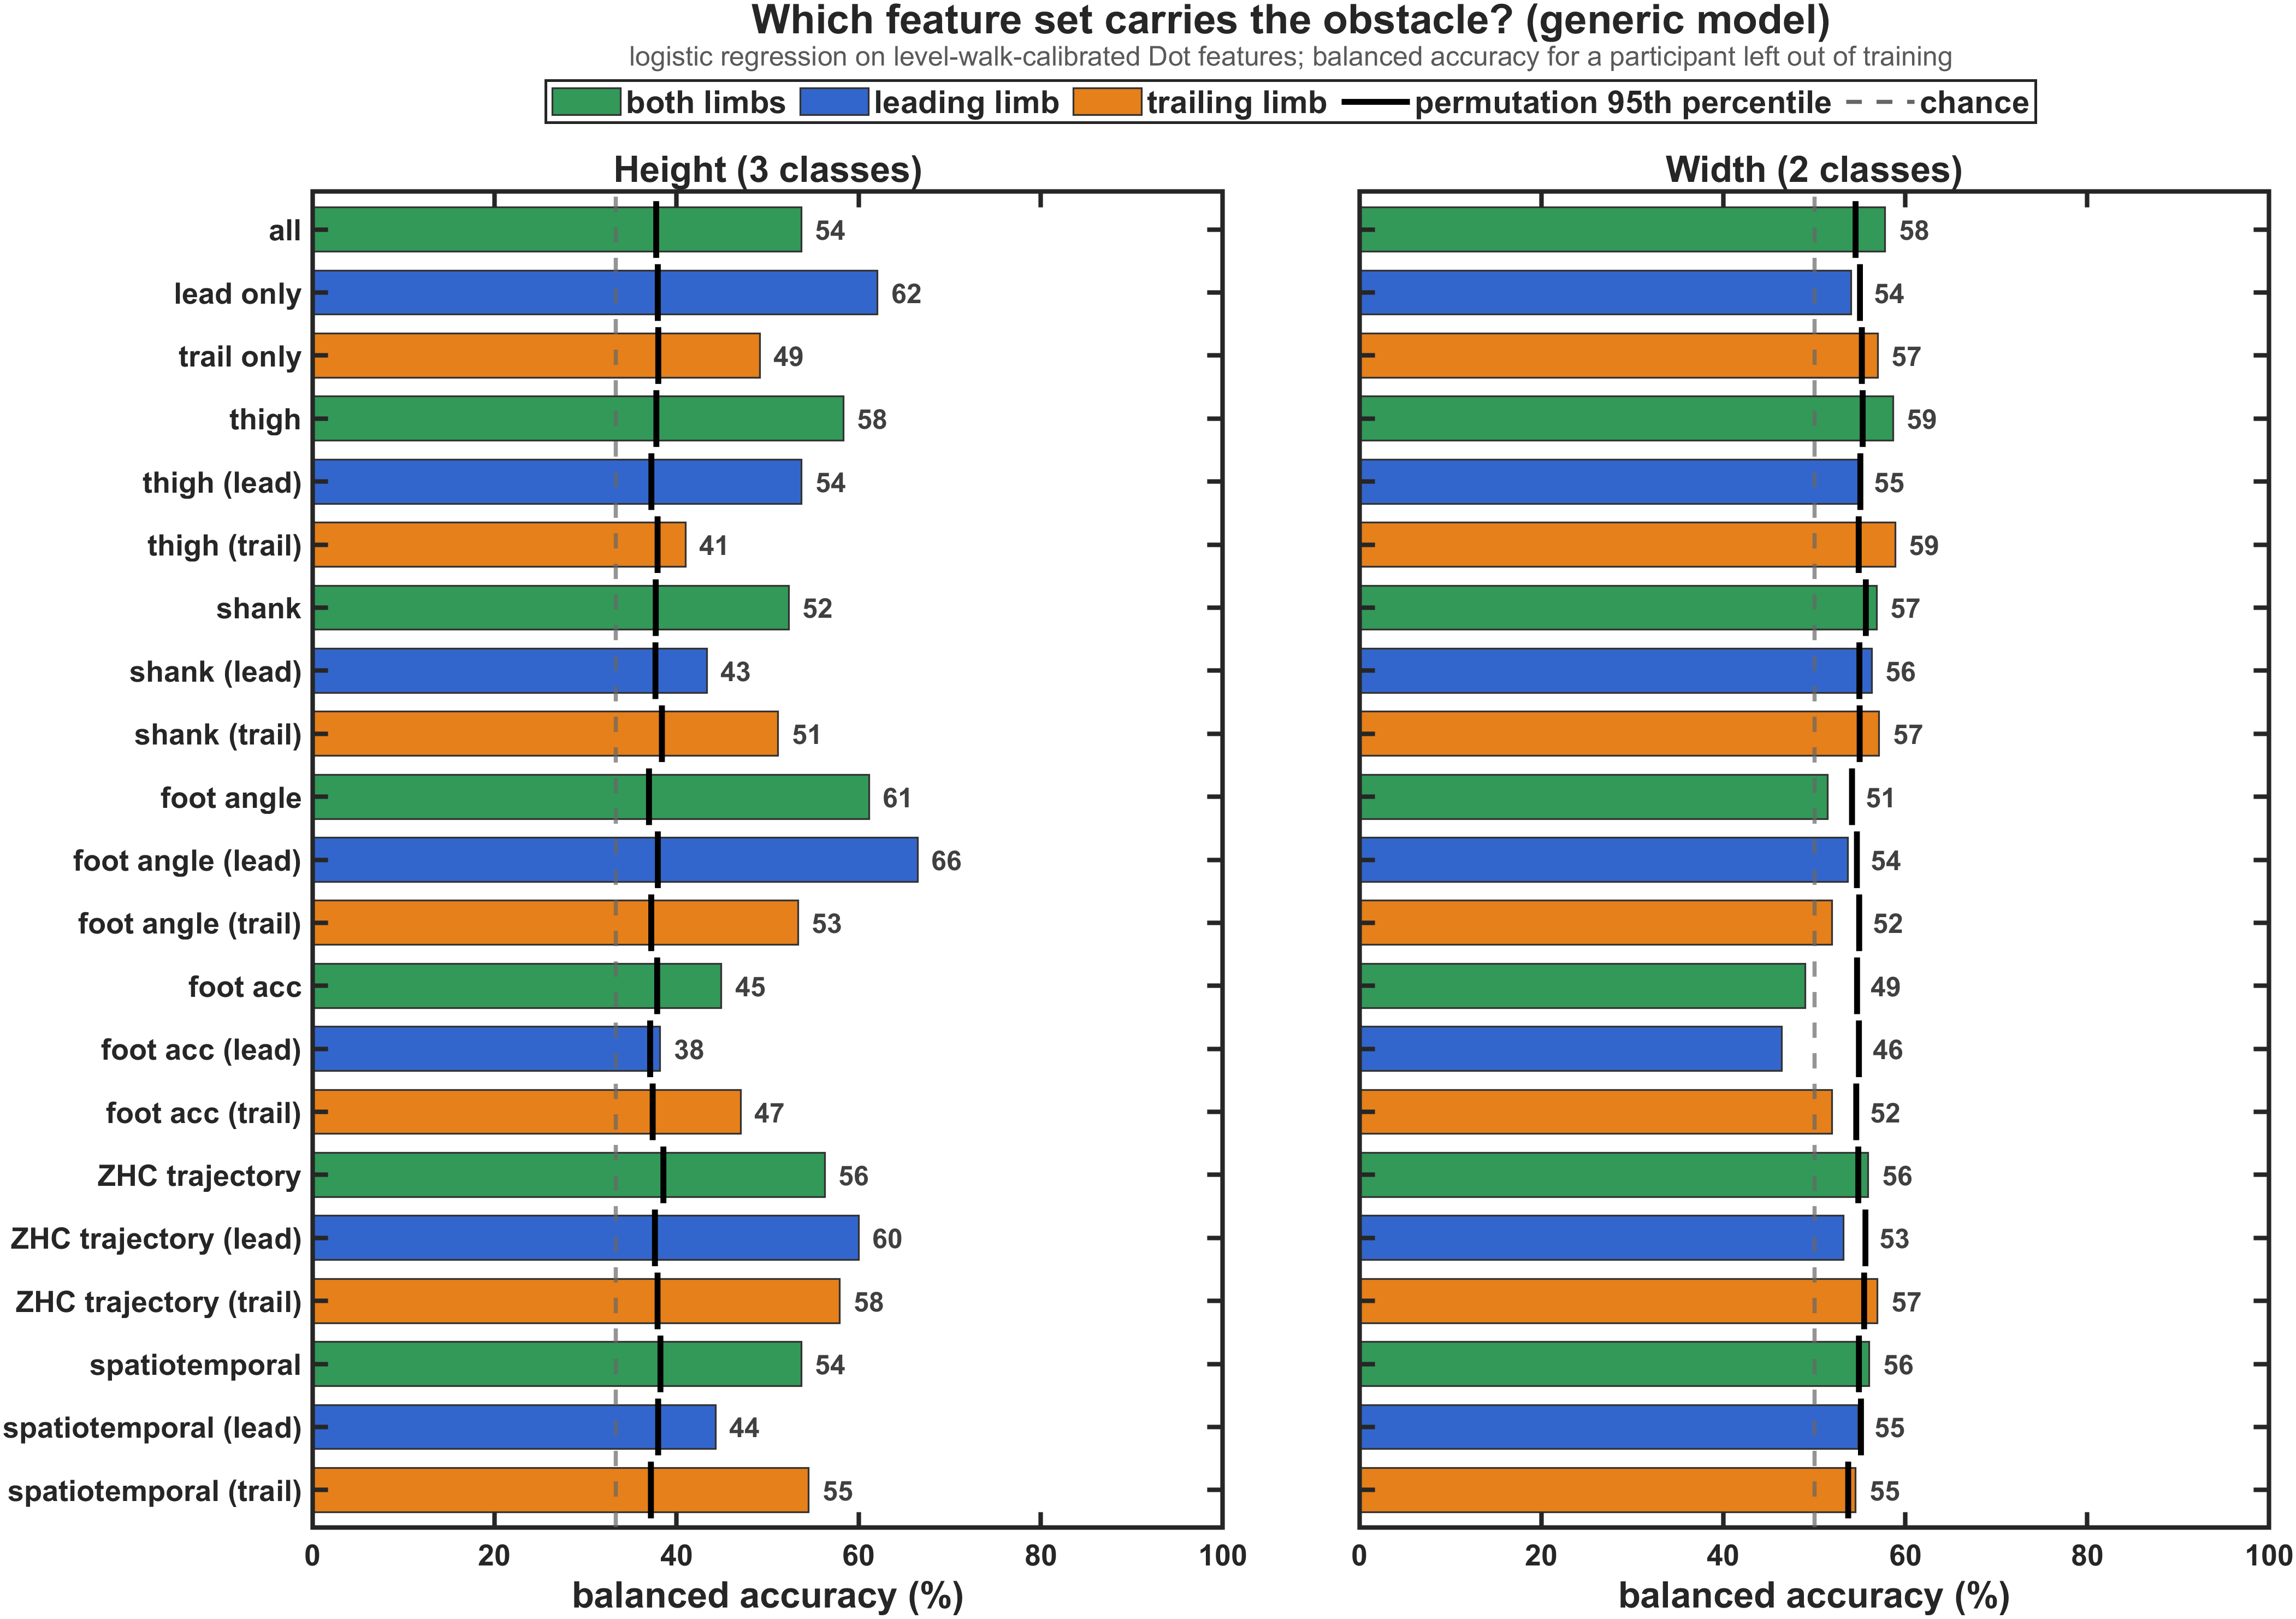
\includegraphics[width=\textwidth]{fig_feature_sets.png}
\caption{Generic model (logistic regression, level-walk calibration) for each Dot feature set: balanced accuracy for an unseen
participant, height (left) and width (right). Bar colour = limb of the set (blue = leading, orange = trailing, green = both);
black tick = 95th percentile of the permutation null (labels shuffled within participant); dashed = chance.}
\label{fig:featuresets}
\end{figure}

\begin{table}[htbp]
\centering
\caption{Height accuracy per segment and limb with person scaling (logistic regression and random forest).}
\label{tab:segments}
\begin{adjustbox}{max width=\textwidth}
{\footnotesize
\begin{tabular}{lrrr}
\toprule
\textbf{features} & \textbf{n feat} & \textbf{logistic (C = 0.1)} & \textbf{random forest} \\
\midrule
lead only & 57 & 79.6\% (73--86) & 88.4\% (83--93) \\
trail only & 52 & 78.0\% (67--87) & 86.5\% (79--92) \\
thigh & 24 & 73.4\% (65--80) & 77.6\% (66--87) \\
thigh (lead) & 12 & 78.0\% (68--87) & 77.4\% (67--85) \\
thigh (trail) & 12 & 47.4\% (39--55) & 44.2\% (35--53) \\
shank & 24 & 69.6\% (62--76) & 79.4\% (69--88) \\
shank (lead) & 12 & 45.2\% (39--52) & 49.8\% (41--56) \\
shank (trail) & 12 & 72.7\% (65--79) & 78.2\% (68--86) \\
foot angle & 26 & 84.7\% (77--91) & 88.1\% (83--93) \\
foot angle (lead) & 13 & 83.9\% (79--89) & 88.1\% (84--92) \\
foot angle (trail) & 13 & 75.5\% (67--83) & 83.4\% (75--90) \\
foot acc & 6 & 51.4\% (43--61) & 58.0\% (49--67) \\
foot acc (lead) & 3 & 34.1\% (29--39) & 36.9\% (30--44) \\
foot acc (trail) & 3 & 52.3\% (43--61) & 54.0\% (46--62) \\
ZHC trajectory & 22 & 88.4\% (83--93) & 89.2\% (83--94) \\
ZHC trajectory (lead) & 11 & 81.2\% (78--85) & 84.9\% (80--89) \\
ZHC trajectory (trail) & 11 & 82.3\% (74--89) & 84.5\% (75--92) \\
spatiotemporal & 10 & 68.7\% (59--77) & 71.6\% (63--80) \\
spatiotemporal (lead) & 7 & 54.3\% (47--62) & 55.4\% (50--62) \\
spatiotemporal (trail) & 2 & 68.4\% (60--77) & 66.5\% (59--74) \\
\bottomrule
\end{tabular}
}
\end{adjustbox}

\end{table}

\subsubsection{When the height is known}

Using only the leading limb's data available up to a given moment of its swing (Table~\ref{tab:timing},
Figure~\ref{fig:settings}), the person-scaled forest already reaches 52\,\% at the leading toe-off, about 80\,\% by its apex
(50\,\% of the swing, a median 458\,ms before the trailing toe leaves the floor) and 88.5\,\% at 70\,\% of the swing (355\,ms
before). The generic model stays at 41--65\,\%. With logistic regression (Figure~\ref{fig:cueing}) the generic model rises
from 42\,\% at the leading toe-off to about 60\,\% by the leading foot apex and stays there.

\begin{table}[htbp]
\centering
\caption{Height from the leading limb's data up to $x$\,\% of its swing, with the median time left before the trailing toe
lift-off (camera).}
\label{tab:timing}
\begin{adjustbox}{max width=\textwidth}
{\footnotesize
\begin{tabular}{lrrrrr}
\toprule
\textbf{data up to} & \textbf{ms before the trailing lift-off} & \textbf{level, logistic} & \textbf{level, forest} & \textbf{self, logistic} & \textbf{self, forest} \\
\midrule
0\% & 733 & 42.0\% & 41.2\% & 46.7\% & 52.1\% \\
10\% & 682 & 50.0\% & 48.0\% & 58.3\% & 63.8\% \\
20\% & 630 & 54.2\% & 53.5\% & 63.8\% & 69.7\% \\
30\% & 573 & 51.8\% & 55.8\% & 65.0\% & 73.8\% \\
40\% & 517 & 58.3\% & 61.2\% & 68.5\% & 79.0\% \\
50\% & 458 & 59.9\% & 62.8\% & 73.5\% & 80.5\% \\
60\% & 410 & 61.5\% & 64.6\% & 77.4\% & 80.4\% \\
70\% & 355 & 58.7\% & 64.0\% & 83.9\% & 88.5\% \\
80\% & 303 & 60.2\% & 62.4\% & 82.0\% & 86.5\% \\
90\% & 248 & 58.1\% & 55.6\% & 81.4\% & 86.8\% \\
100\% & 200 & 59.4\% & 57.0\% & 80.7\% & 85.8\% \\
\bottomrule
\end{tabular}
}
\end{adjustbox}

\end{table}

\begin{figure}[htbp]
\centering
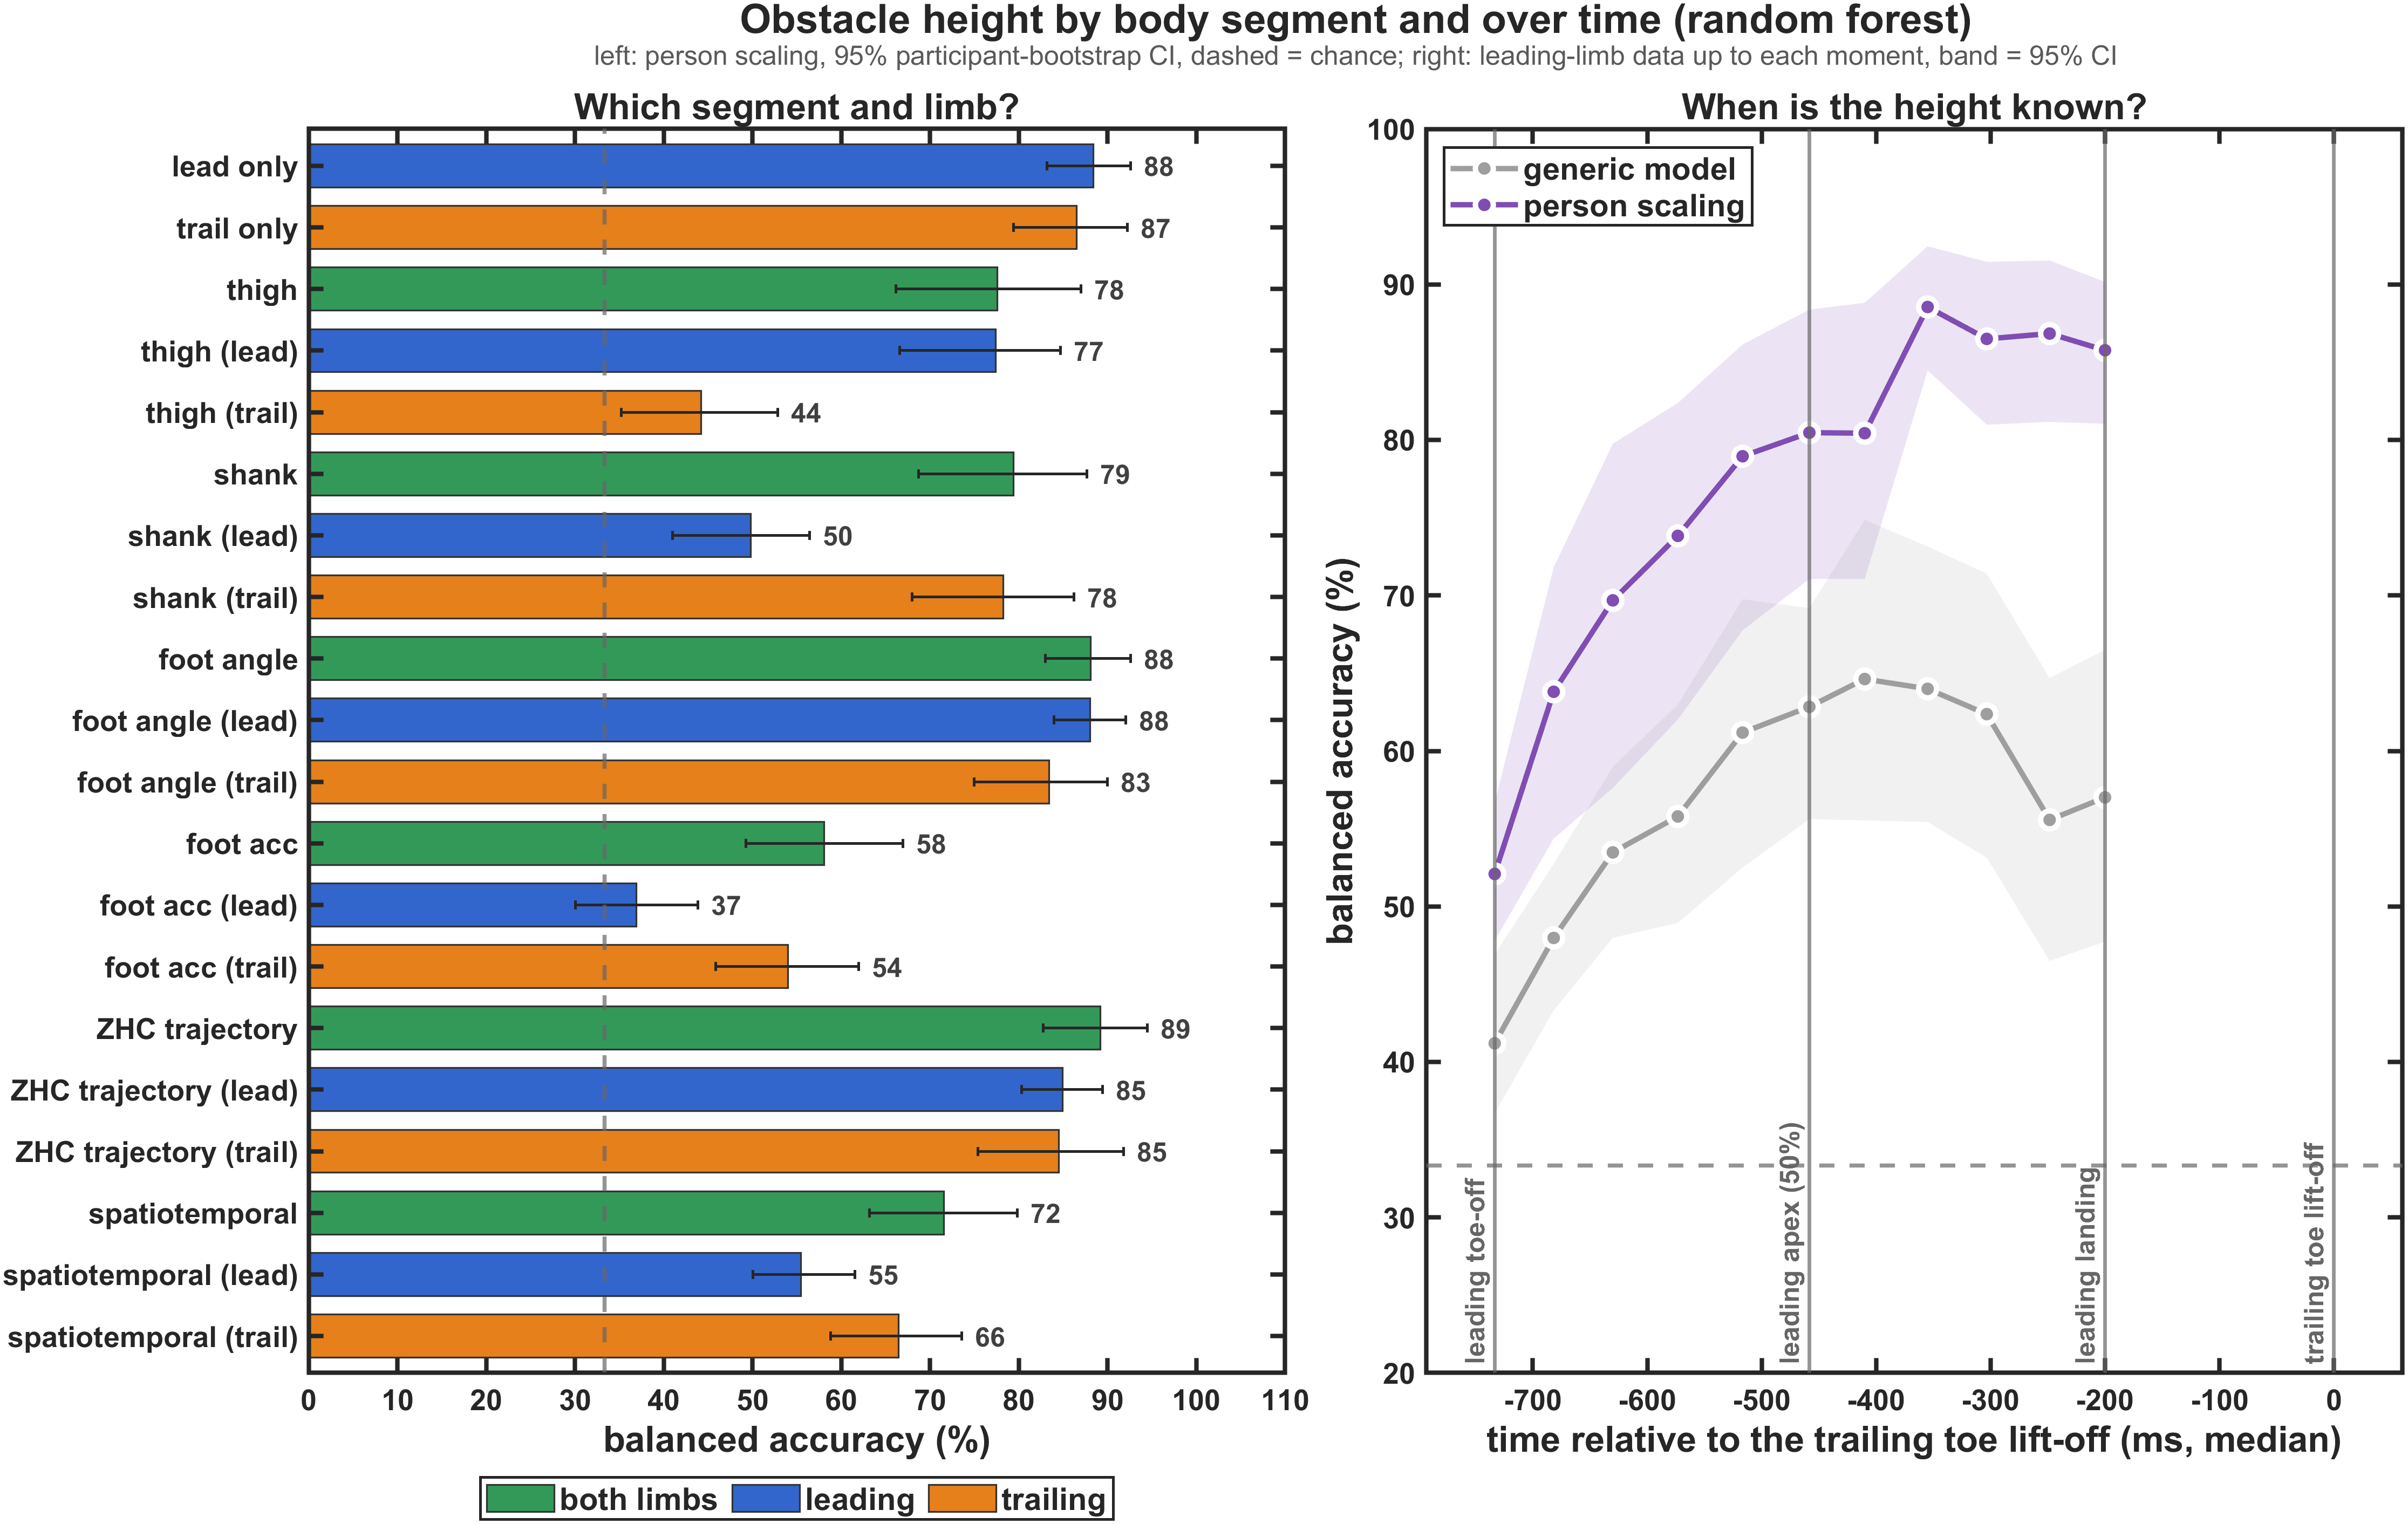
\includegraphics[width=\textwidth]{fig_settings.png}
\caption{Left: height accuracy by segment and limb with person scaling (random forest; blue = leading, orange = trailing,
green = both limbs; 95\,\% CI). Right: height from the leading-limb data available so far, generic (grey) vs person scaling (purple),
against the median time relative to the trailing toe lift-off (band = 95\,\% CI).}
\label{fig:settings}
\end{figure}

\begin{figure}[htbp]
\centering
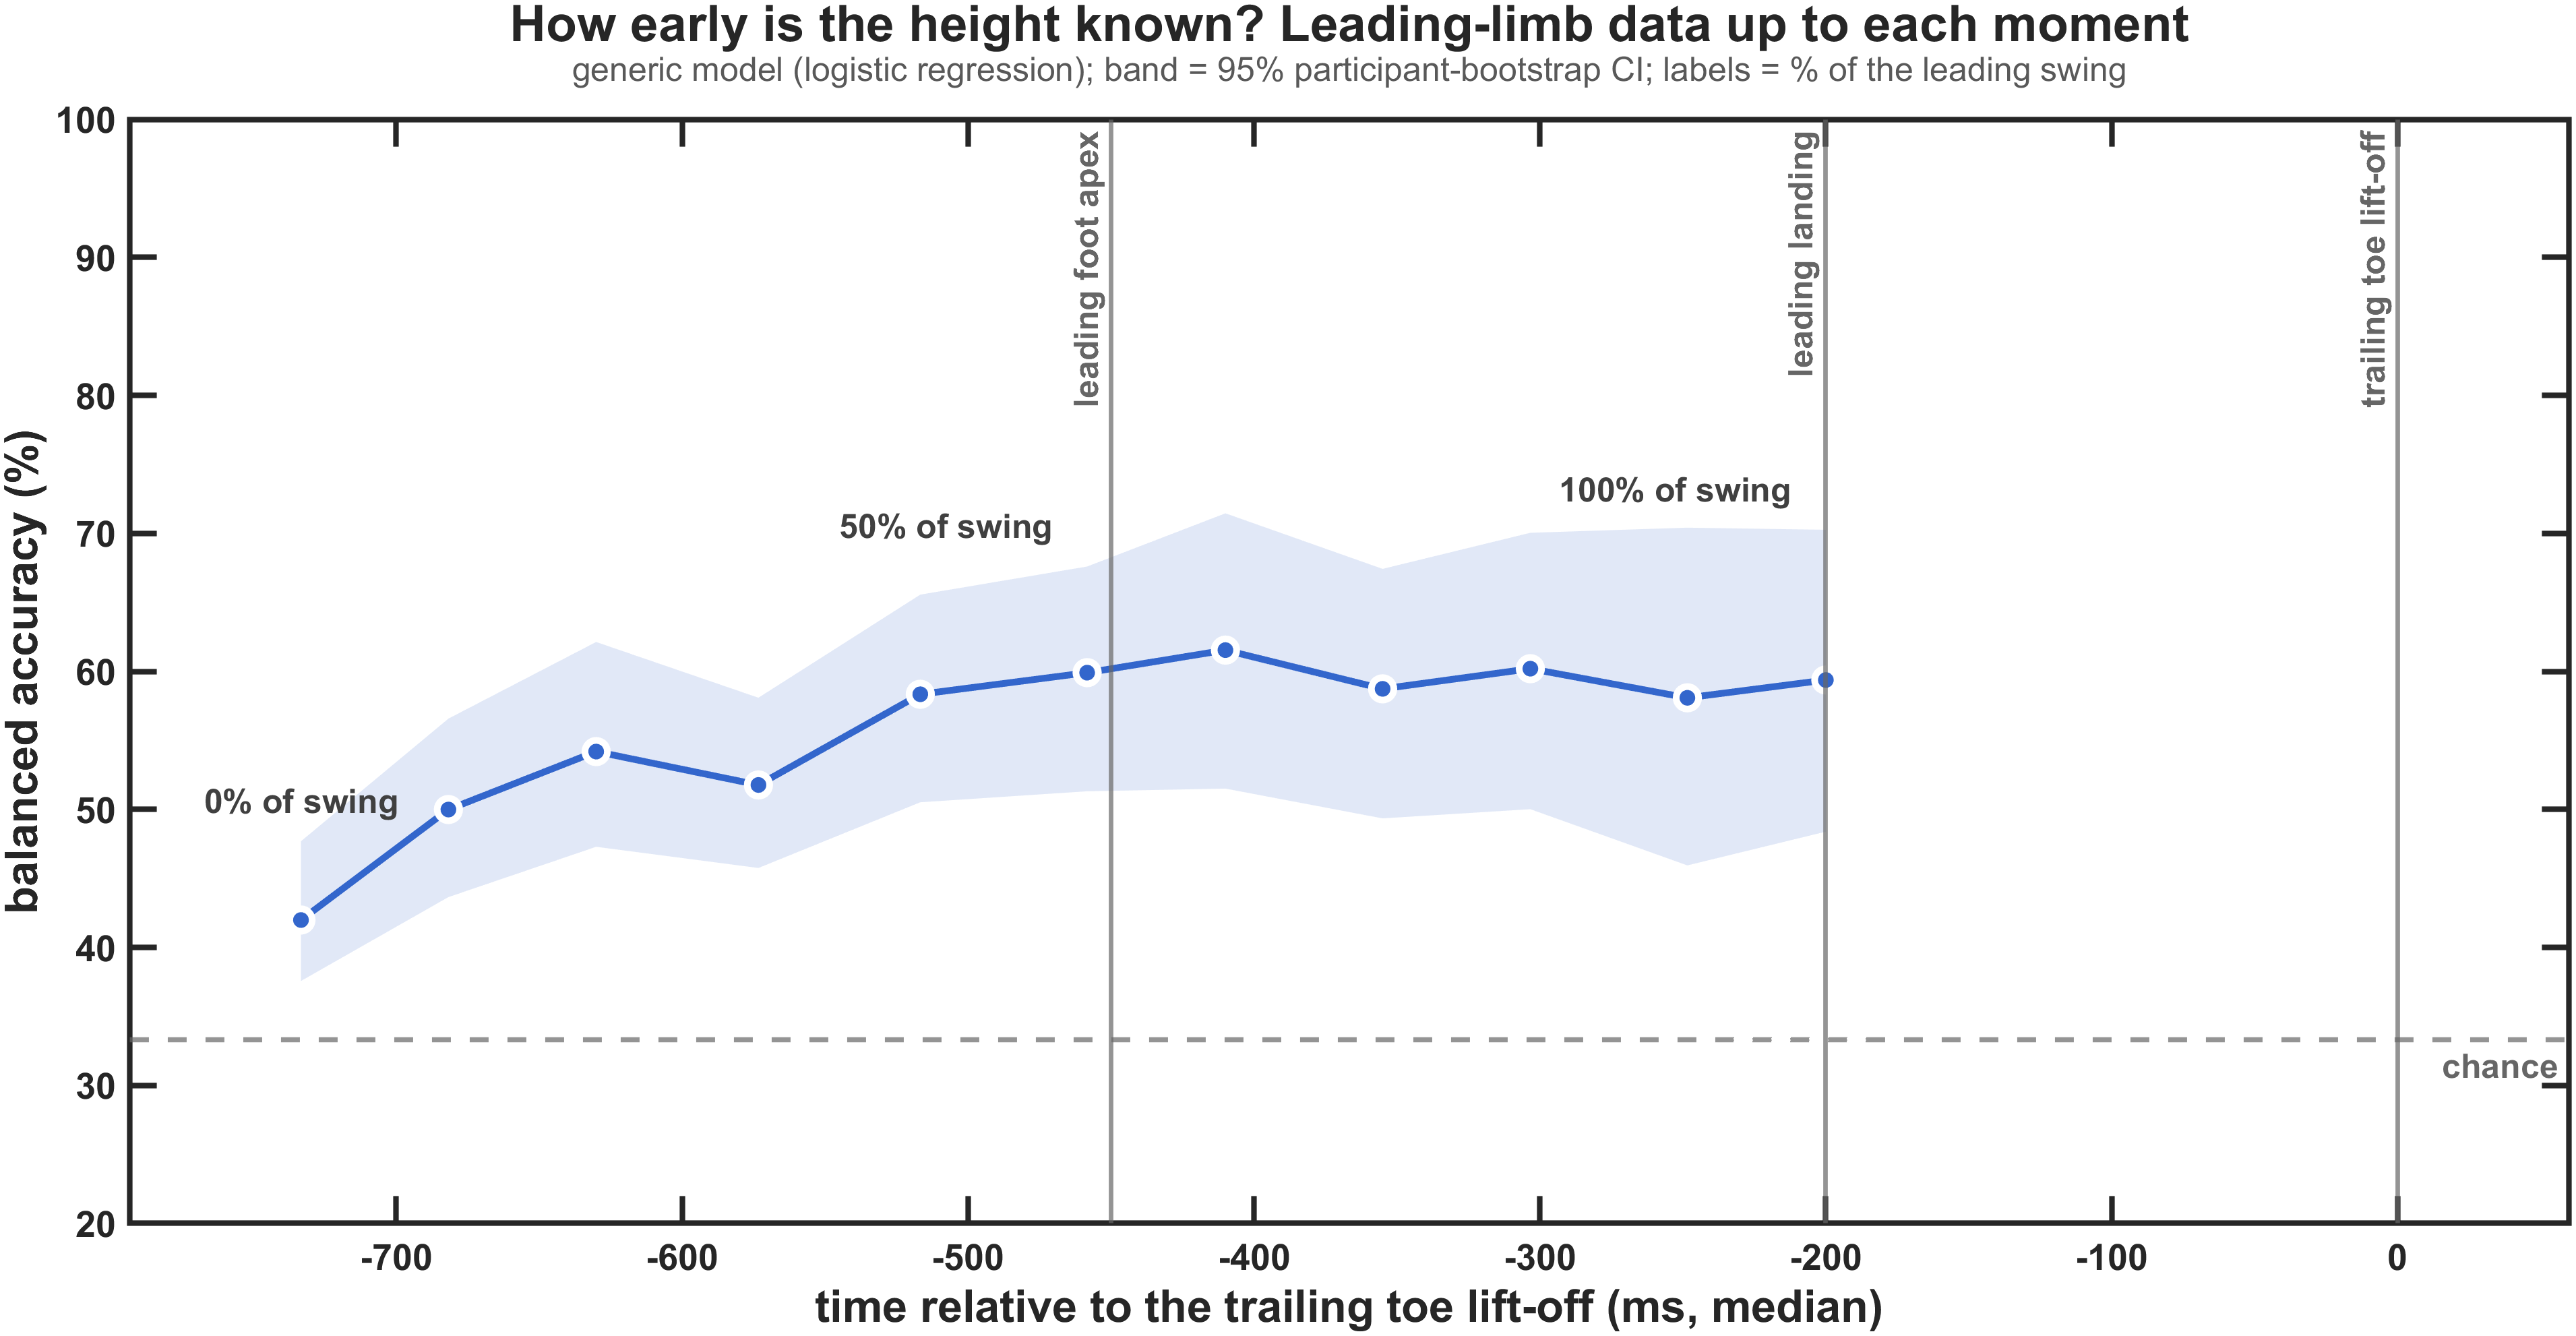
\includegraphics[width=\textwidth]{fig_cueing_time.png}
\caption{Generic model (logistic regression) using the leading-limb data available up to each moment of its swing (labels = \% of the
swing), against the median time relative to the trailing toe lift-off. Band = 95\,\% participant-bootstrap CI; vertical lines =
median leading foot apex, leading landing and trailing toe lift-off; dashed = chance.}
\label{fig:cueing}
\end{figure}

\subsubsection{Height as a number}

Regressing the obstacle height in centimetres (Table~\ref{tab:cm}), the person-scaled forest vote has a mean absolute error of
2.39\,cm ($r = 0.91$); rounding to the nearest of the person's three nominal heights gives 84.8\,\%. Neighbouring heights are
8.3--10.6\,cm apart, so the typical error is about a quarter of a step.

\begin{table}[htbp]
\centering
\caption{Obstacle height in centimetres (regression), and the class nearest to the estimate.}
\label{tab:cm}
\begin{adjustbox}{max width=\textwidth}
{\footnotesize
\begin{tabular}{llrrr}
\toprule
\textbf{inputs} & \textbf{model} & \textbf{MAE (cm)} & \textbf{r} & \textbf{class from cm (bal. acc)} \\
\midrule
lead, level & ridge & 5.19 & 0.69 & 63.5\% \\
lead, level & forest & 4.19 & 0.72 & 61.7\% \\
lead, self & ridge & 3.51 & 0.79 & 76.8\% \\
lead, self & forest & 2.42 & 0.88 & 83.3\% \\
lead + trail vote, self & ridge & 3.32 & 0.84 & 76.7\% \\
lead + trail vote, self & forest & 2.39 & 0.91 & 84.8\% \\
\bottomrule
\end{tabular}
}
\end{adjustbox}

\end{table}

\subsubsection{Per participant, and two easier tasks}

With person scaling the accuracy is 83--100\,\% for nine participants and 73\,\% for participant 108
(Table~\ref{tab:perparticipant}; the reason is shown in Section~\ref{sec:res-device}). Two related tasks are solved almost
perfectly by the Dot: telling the leading from the trailing limb's swing (100\,\%, Table~\ref{tab:leadtrail}) and telling an
obstacle crossing from a level-walk stride (100\,\%, Table~\ref{tab:obslevel}).

The generic model varies much more between people (Figure~\ref{fig:participants}): 31--74\,\% with all features and 42--85\,\% with
the leading limb only. Participant 108 reaches 85\,\% from the leading limb alone but only 38\,\% with all features and 31\,\% with
the trailing limb, whose lift is the least consistent in the group (Section~\ref{sec:res-device}).

\begin{figure}[htbp]
\centering
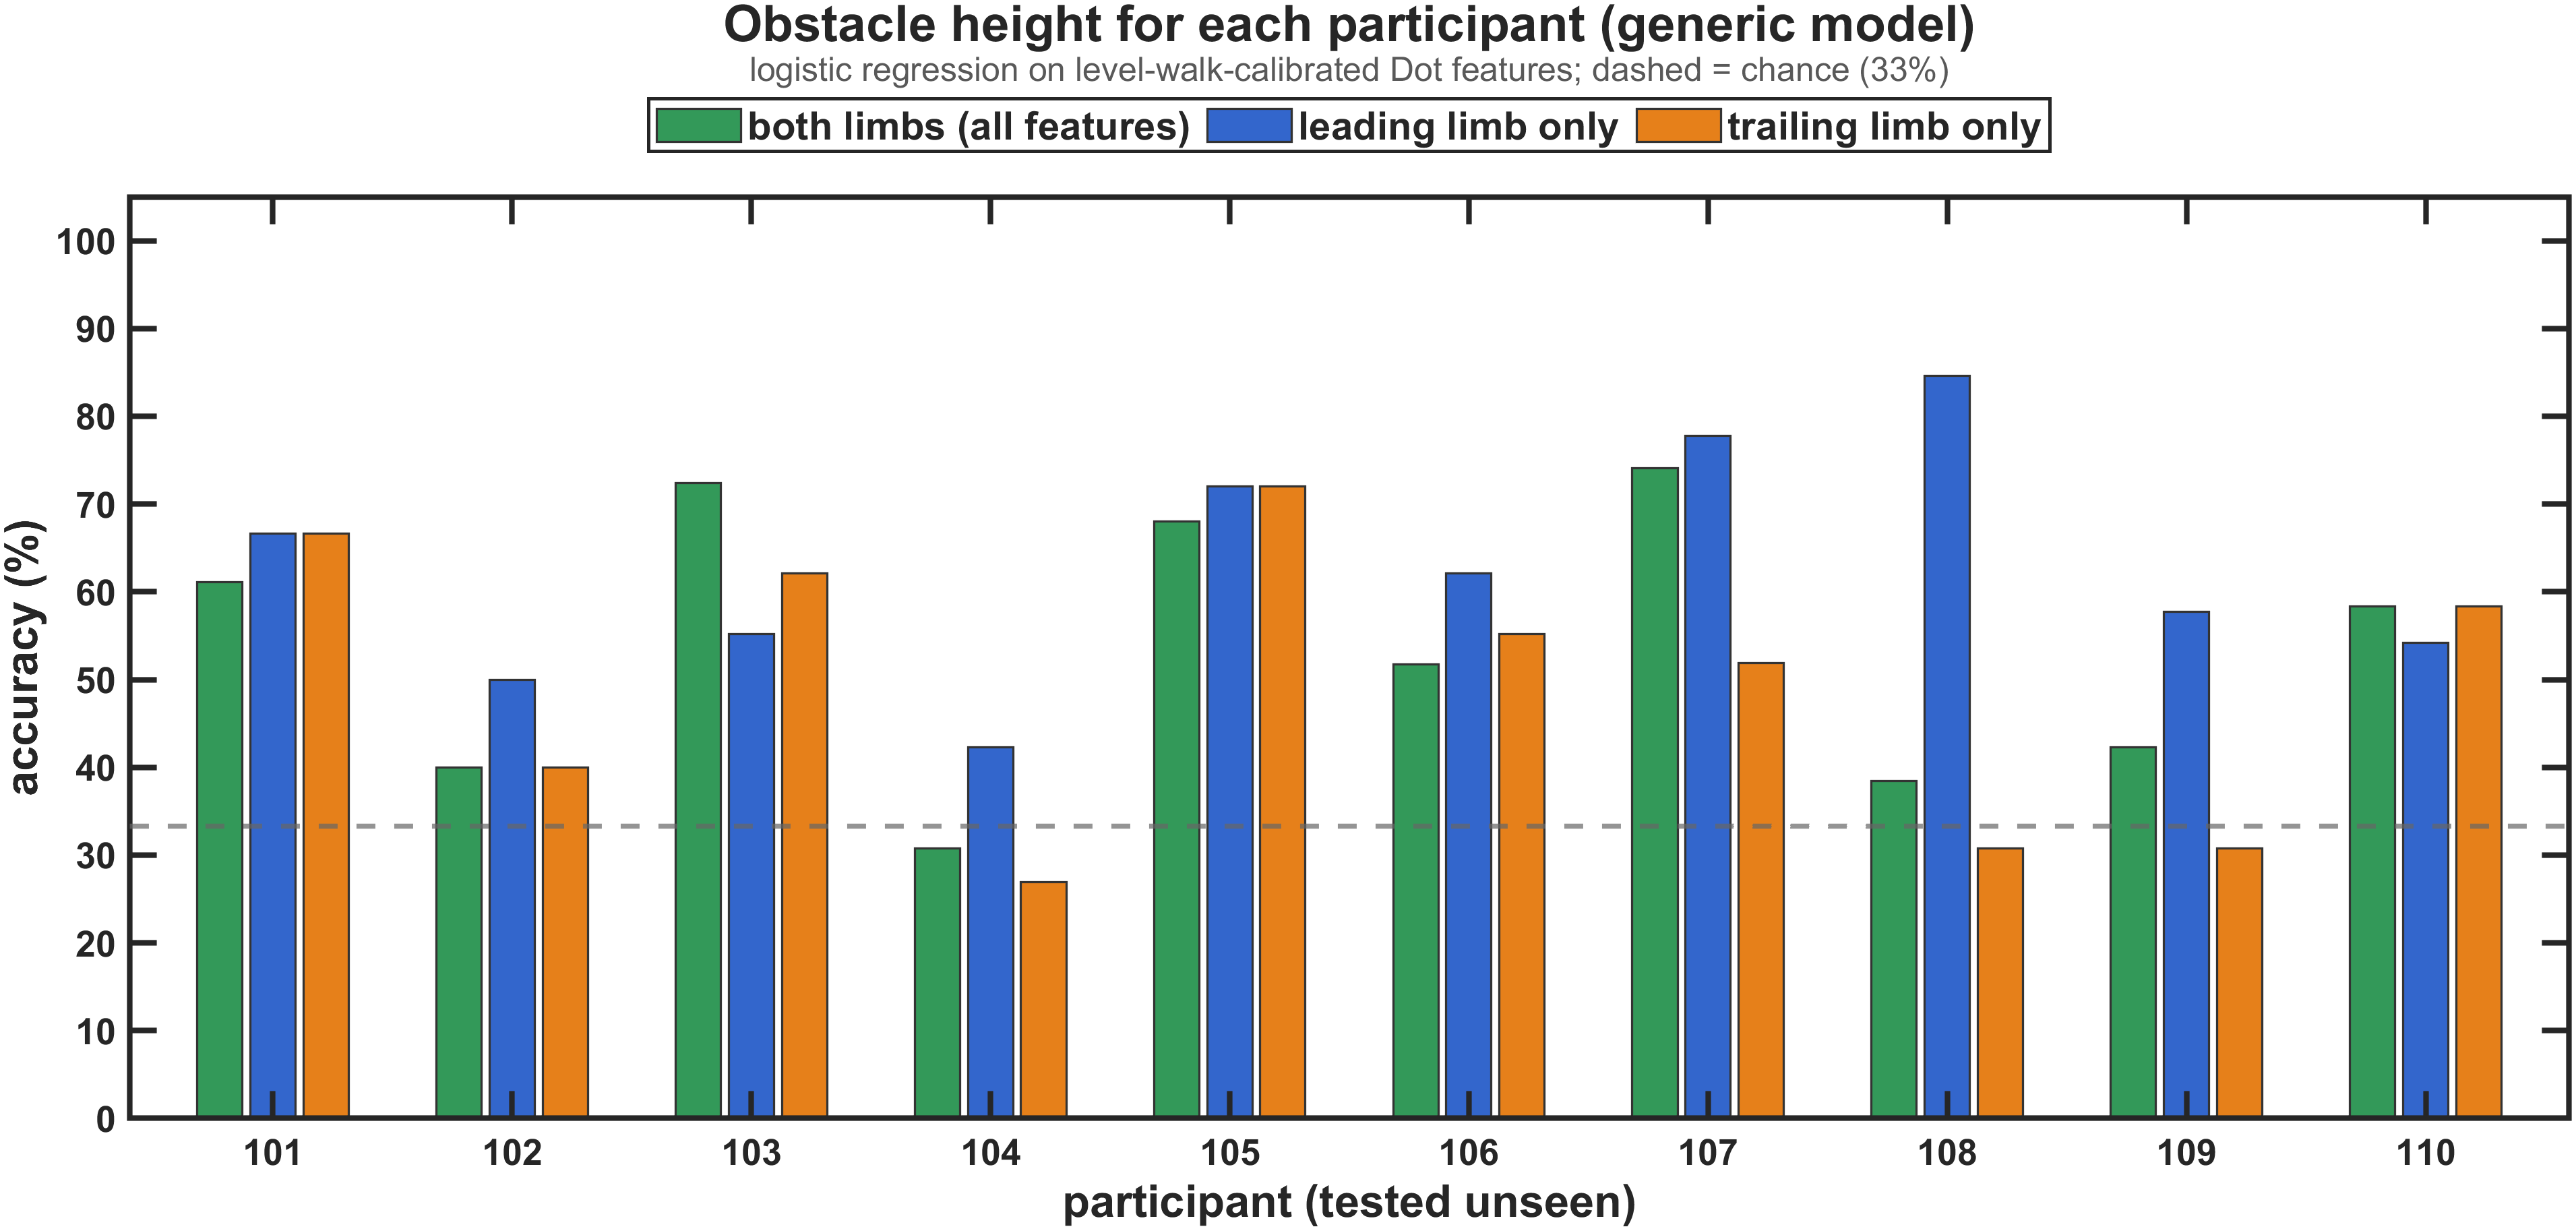
\includegraphics[width=\textwidth]{fig_participants.png}
\caption{Generic model (logistic regression) for each participant when left out of training: all features (green), the leading limb
only (blue) and the trailing limb only (orange). Dashed = chance.}
\label{fig:participants}
\end{figure}

\begin{table}[htbp]
\centering
\caption{Height accuracy for each left-out participant.}
\label{tab:perparticipant}
\begin{adjustbox}{max width=\textwidth}
{\footnotesize
\begin{tabular}{lrrrrrrrrrrr}
\toprule
\textbf{setting} & \textbf{101} & \textbf{102} & \textbf{103} & \textbf{104} & \textbf{105} & \textbf{106} & \textbf{107} & \textbf{108} & \textbf{109} & \textbf{110} & \textbf{overall} \\
\midrule
level, logreg C=0.1, lead & 67\% & 50\% & 55\% & 42\% & 72\% & 62\% & 78\% & 85\% & 58\% & 54\% & 62.1\% \\
self, logreg C=0.1, lead & 94\% & 57\% & 90\% & 92\% & 84\% & 83\% & 70\% & 73\% & 77\% & 83\% & 79.6\% \\
self, forest, lead & 94\% & 70\% & 97\% & 92\% & 92\% & 83\% & 89\% & 88\% & 92\% & 92\% & 88.4\% \\
self, forest, fusion & 94\% & 83\% & 97\% & 96\% & 100\% & 93\% & 85\% & 73\% & 88\% & 96\% & 90.4\% \\
\bottomrule
\end{tabular}
}
\end{adjustbox}

\end{table}

\begin{table}[htbp]
\centering
\begin{minipage}{0.48\textwidth}
\centering
\caption{Leading or trailing limb, from one swing.}
\label{tab:leadtrail}
\begin{adjustbox}{max width=\textwidth}
{\footnotesize
\begin{tabular}{llrrr}
\toprule
\textbf{norm} & \textbf{model} & \textbf{bal. acc} & \textbf{95\% CI} & \textbf{perm p} \\
\midrule
raw & logreg & 100.0\% & 100--100 & 0.003 \\
raw & forest & 100.0\% & 100--100 & - \\
level & logreg & 100.0\% & 100--100 & 0.003 \\
level & forest & 100.0\% & 100--100 & - \\
self & logreg & 100.0\% & 100--100 & 0.003 \\
self & forest & 100.0\% & 100--100 & - \\
\bottomrule
\end{tabular}
}
\end{adjustbox}

\end{minipage}\hfill
\begin{minipage}{0.48\textwidth}
\centering
\caption{Obstacle crossing or level-walk stride.}
\label{tab:obslevel}
\begin{adjustbox}{max width=\textwidth}
{\footnotesize
\begin{tabular}{llrrr}
\toprule
\textbf{norm} & \textbf{model} & \textbf{lead} & \textbf{trail} & \textbf{fusion} \\
\midrule
raw & logreg & 100.0\% (100--100) & 97.1\% (92--100) & 100.0\% (100--100) \\
raw & forest & 99.8\% (99--100) & 99.8\% (99--100) & 100.0\% (100--100) \\
self & logreg & 94.9\% (84--100) & 100.0\% (100--100) & 100.0\% (100--100) \\
self & forest & 100.0\% (100--100) & 99.8\% (99--100) & 100.0\% (100--100) \\
\bottomrule
\end{tabular}
}
\end{adjustbox}

\end{minipage}
\end{table}

\subsubsection{Generalisation to obstacles not seen in training}
\label{sec:res-general}

\paragraph{Unseen heights.} Real obstacles have arbitrary heights, so the regression was also trained with one height level removed
from the training data (Table~\ref{tab:unseenheight}). Interpolation works: a ridge model that never saw the middle height (H2)
estimates it with a 3.1\,cm mean absolute error and puts 79\,\% of those crossings at the right level (88\,\% when trained on all
heights). Extrapolation is biased toward the trained range: an unseen lowest or highest height is over- or under-estimated by about
half a step (+4.0 and $-5.7$\,cm). The random forest cannot extrapolate at all (an unseen H1 or H3 is off by a full step), and the
generic models are worse throughout. A device for obstacles of any height should therefore be trained on obstacles that span the
heights it will meet, with a model that scales linearly with height.

\begin{table}[htbp]
\centering
\caption{Height in cm when a height level is missing from training (person scaling). Cells: mean absolute error in cm (mean signed
error, + = too high); ``right level'' = the estimate is closest to the person's true nominal height.}
\label{tab:unseenheight}
\input{tables/validate_unseen_height}
\end{table}

\paragraph{Unseen width.} Height recognition trained on crossings of one width only and tested on the other width loses about
6.5 points compared with training on the same width with the same amount of data (86.2\,\% vs 92.7\,\%, Table~\ref{tab:unseenwidth}):
although width itself is barely recognisable, the obstacle depth slightly changes how the height shows in the foot motion, so
training data should include obstacles of different depths.

\begin{table}[htbp]
\centering
\caption{Height recognition tested on one width, trained on the same width, the other width only, or both (two foot IMUs, person
scaling, forest vote).}
\label{tab:unseenwidth}
\input{tables/validate_unseen_width}
\end{table}

\input{sections/04b3_whatmodel}


\subsection{Obstacle width}
\label{sec:res-width}

Width (5 vs 15\,cm, chance 50\,\%) is recognised only slightly above chance with any input or model: 54--65\,\% with the Dot
summary features (Table~\ref{tab:limbs}) and at most 66\,\% with new width-specific features (Table~\ref{tab:explorewidth}).
The generic model recognises the 5\,cm obstacle in 62\,\% and the 15\,cm one in 53\,\% of crossings (Figure~\ref{fig:confusion}, right).
For all six obstacles, person scaling reaches 61\,\% (chance 17\,\%); the errors are almost all between the two widths of the
same height (Table~\ref{tab:sixconf}).

\begin{table}[htbp]
\centering
\caption{Width with new features (person scaling): clearance-shape features, step-relative ratios and their combination.}
\label{tab:explorewidth}
\begin{adjustbox}{max width=\textwidth}
{\footnotesize
\begin{tabular}{lllrrr}
\toprule
\textbf{features} & \textbf{norm} & \textbf{model} & \textbf{lead} & \textbf{trail} & \textbf{fusion} \\
\midrule
summary & self & logreg & 64.6\% (63--67; worst 60\%) & 58.5\% (53--65; worst 46\%) & 64.3\% (59--69; worst 50\%) \\
summary & self & boost & 60.9\% (56--66; worst 48\%) & 60.4\% (56--65; worst 46\%) & 61.2\% (56--67; worst 46\%) \\
shape & self & logreg & 56.8\% (51--61; worst 41\%) & 64.6\% (59--71; worst 52\%) & 64.6\% (58--71; worst 44\%) \\
ratio & self & logreg & 59.5\% (52--65; worst 37\%) & 60.2\% (55--66; worst 45\%) & 62.6\% (56--68; worst 42\%) \\
ratio + summary & self & logreg & 62.7\% (59--66; worst 54\%) & 62.7\% (57--69; worst 50\%) & 66.2\% (61--72; worst 57\%) \\
\bottomrule
\end{tabular}
}
\end{adjustbox}

\end{table}

\begin{table}[htbp]
\centering
\caption{Six-obstacle confusion matrix (person scaling, forest, soft vote; rows = true obstacle W[width]H[height]).}
\label{tab:sixconf}
\begin{adjustbox}{max width=\textwidth}
{\footnotesize
\begin{tabular}{lrrrrrr}
\toprule
\textbf{true \textbackslash{}\textbackslash{} pred} & \textbf{W1H1} & \textbf{W1H2} & \textbf{W1H3} & \textbf{W2H1} & \textbf{W2H2} & \textbf{W2H3} \\
\midrule
W1H1 & 32 & 0 & 0 & 12 & 0 & 0 \\
W1H2 & 0 & 24 & 3 & 1 & 13 & 1 \\
W1H3 & 0 & 2 & 20 & 0 & 5 & 14 \\
W2H1 & 15 & 3 & 0 & 26 & 0 & 0 \\
W2H2 & 0 & 14 & 7 & 0 & 27 & 0 \\
W2H3 & 0 & 0 & 10 & 0 & 1 & 30 \\
\bottomrule
\end{tabular}
}
\end{adjustbox}

\end{table}

\paragraph{Is the limit the sensor or the behaviour?} The camera sees where the feet are placed relative to the obstacle, which
the IMUs cannot. Even so, the 10\,cm wider obstacle changes the foot placement by only a few centimetres (crossing step
+37\,mm, Table~\ref{tab:storywidth}), and width classified from the camera foot placement reaches only 57.6\,\%. The side-to-side
(out-of-plane) motion of the thigh, shank and foot does not help either (Table~\ref{tab:lateral}, Figure~\ref{fig:lateral}).
The width limit is therefore behavioural: people cross a 5 and a 15\,cm deep obstacle in almost the same way.

\begin{table}[htbp]
\centering
\caption{Effect of width on the foot placement seen by the camera and on the Dot trajectory (W2 $-$ W1, median over participants).}
\label{tab:storywidth}
\begin{adjustbox}{max width=\textwidth}
{\footnotesize
\begin{tabular}{p{5.6cm}rrrr}
\toprule
\textbf{variable} & \textbf{W2 - W1 (median over participants)} & \textbf{range} & \textbf{participants $>$ 0} & \textbf{$\eta^2$ width} \\
\midrule
trail toe before obstacle centre (camera) & +30 mm & $-$21 to +75 & 9 / 10 & 0.05 \\
lead heel after obstacle centre (camera) & +5 mm & $-$82 to +81 & 6 / 10 & 0.00 \\
crossing step, trail toe $\rightarrow$ lead heel (camera) & +37 mm & $-$59 to +65 & 8 / 10 & 0.02 \\
lead toe before centre at its toe-off (camera) & +76 mm & $-$122 to +237 & 7 / 10 & 0.02 \\
trail heel after obstacle centre (camera) & $-$8 mm & $-$54 to +53 & 4 / 10 & 0.00 \\
lead foot apex progression (Dot) & +55 mm & $-$7 to +227 & 7 / 10 & 0.04 \\
lead landing progression (Dot) & +31 mm & $-$87 to +84 & 6 / 10 & 0.01 \\
trail landing progression (Dot) & +37 mm & $-$7 to +86 & 8 / 10 & 0.05 \\
lead $\rightarrow$ trail apex lag (Dot) & +14 ms & $-$29 to +57 & 6 / 10 & 0.01 \\
\bottomrule
\end{tabular}
}
\end{adjustbox}

\end{table}

\paragraph{Side-to-side motion.} A wider obstacle might change the frontal-plane tilt, the twist of the segments or the foot's
sideways path instead of the sagittal motion. It does not: the largest width effect on any out-of-plane feature is 6\,\% of the
within-person variance (Table~\ref{tab:lateral}), width from the out-of-plane features alone is 53--54\,\%, and adding them to the
sagittal features does not improve width or height (Table~\ref{tab:lateralclass}). Figure~\ref{fig:lateral} compares the width
effect sizes of the sagittal and out-of-plane features.

\begin{table}[htbp]
\centering
\caption{Width effect on the out-of-plane features ($\eta^2$ within participant $\times$ height), with the W2 $-$ W1 difference and
the height effect for comparison.}
\label{tab:lateral}
\input{tables/lateral_eta}
\end{table}

\begin{table}[htbp]
\centering
\caption{Width and height classification with out-of-plane features, original sagittal + shape features, and both (person scaling).}
\label{tab:lateralclass}
\input{tables/lateral_class}
\end{table}

\begin{figure}[htbp]
\centering
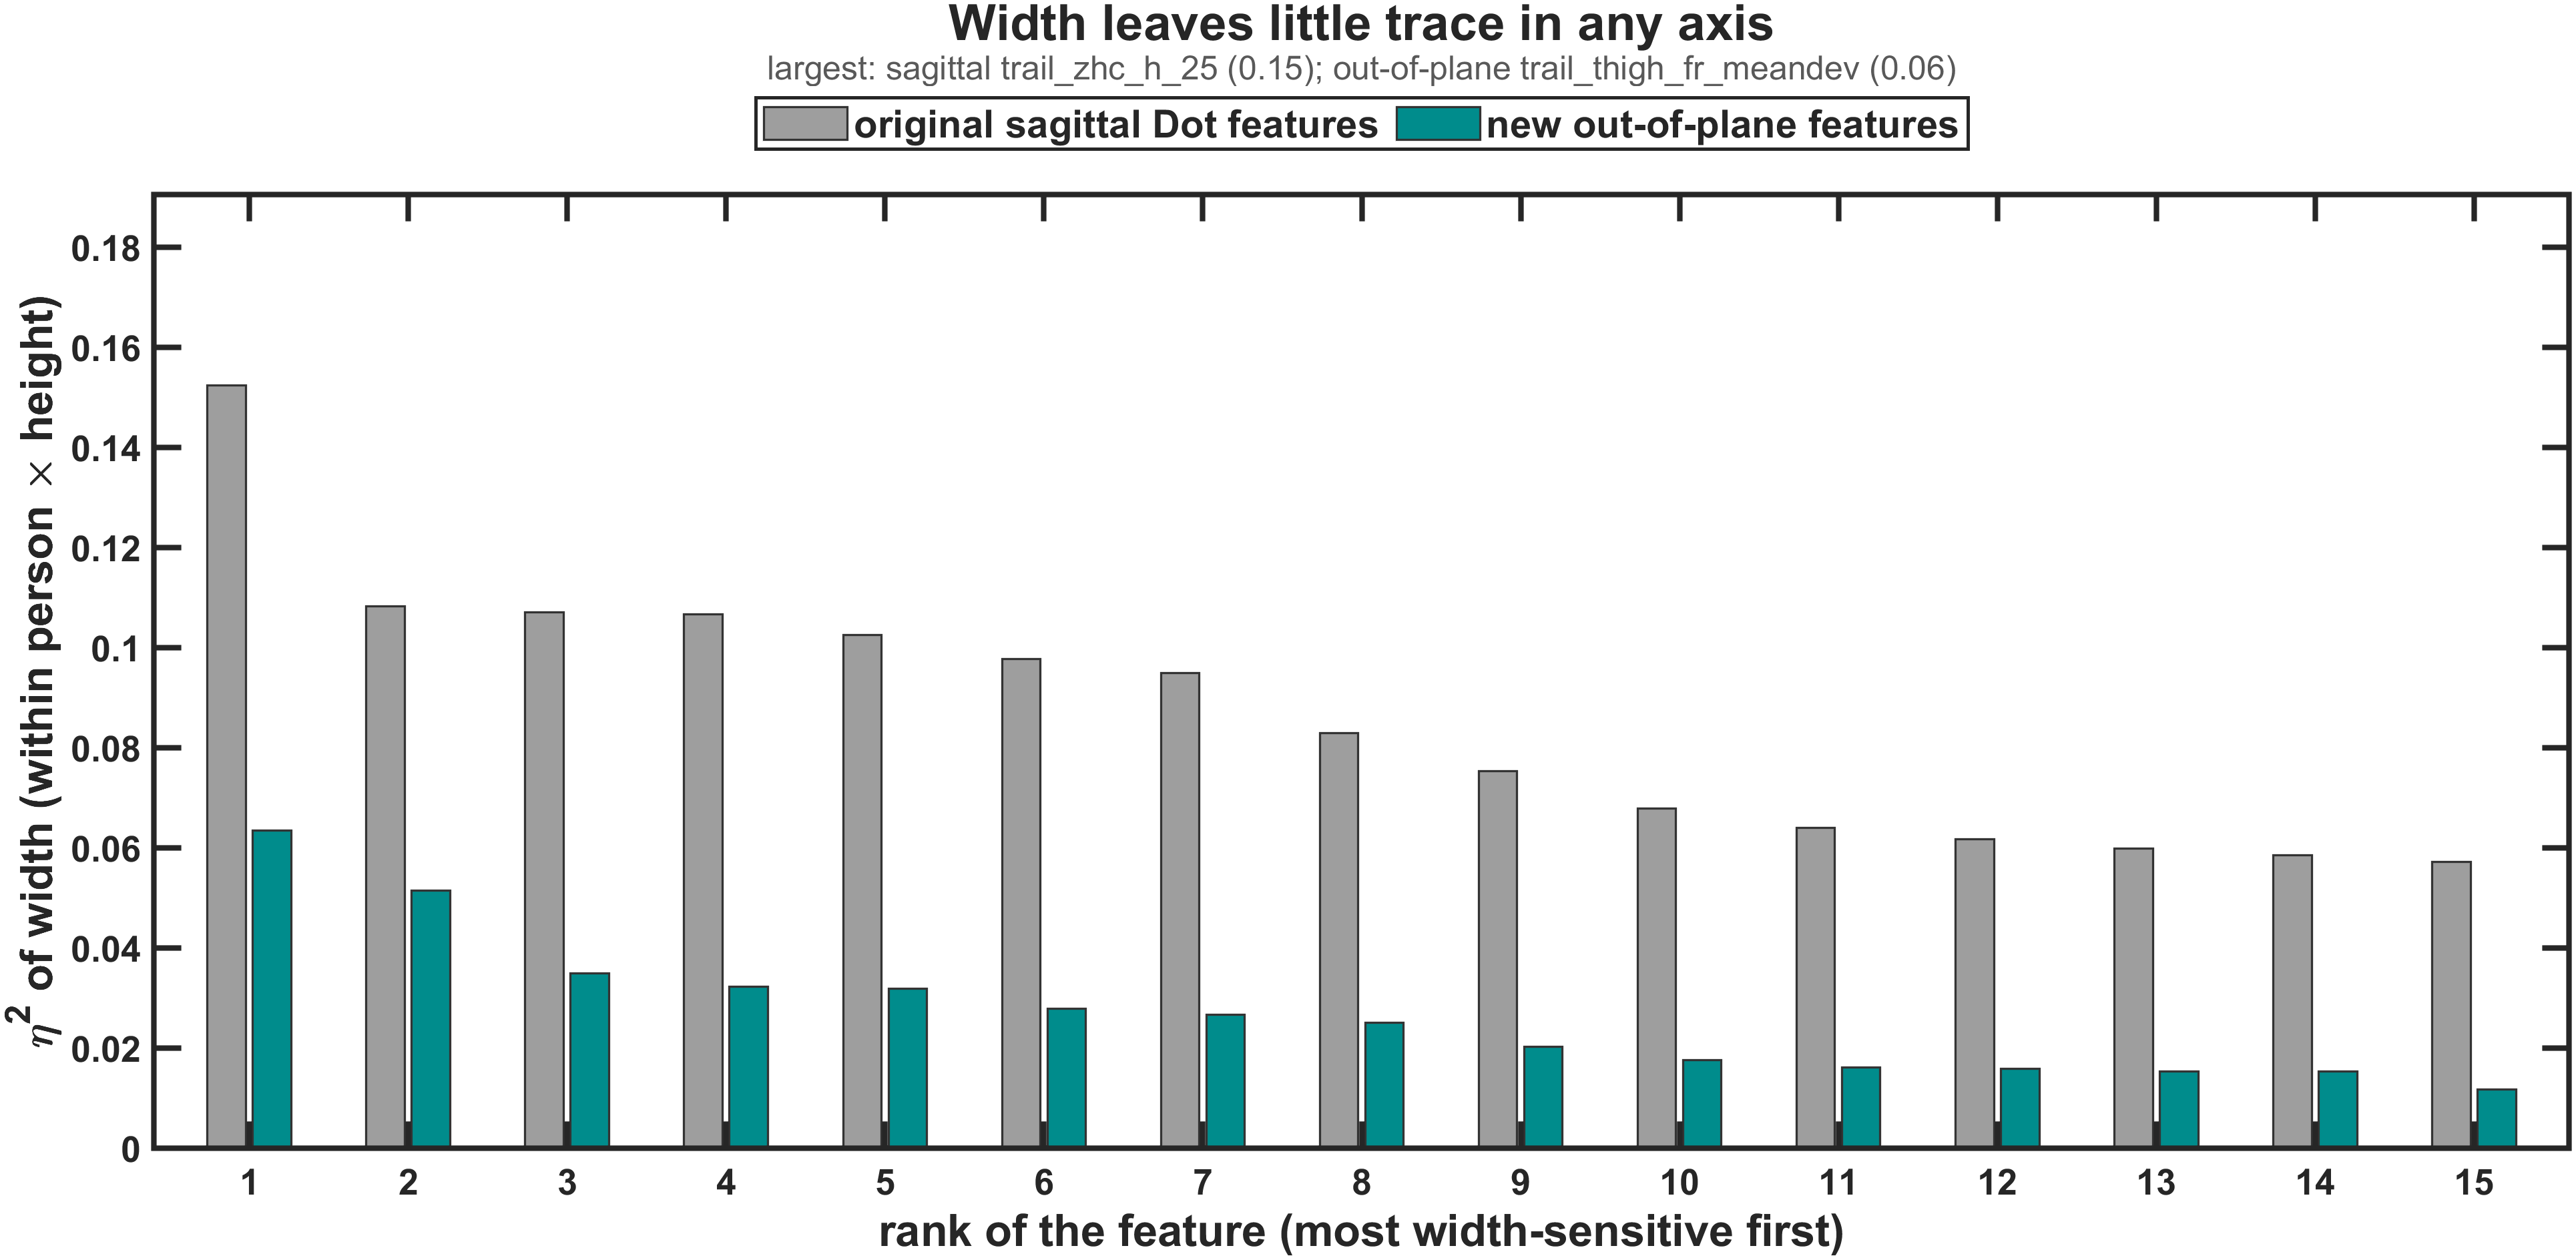
\includegraphics[width=0.9\textwidth]{fig_lateral.png}
\caption{Width effect size ($\eta^2$ within participant $\times$ height) of the 15 most width-sensitive sagittal (grey) and
out-of-plane (teal) features.}
\label{fig:lateral}
\end{figure}


\subsection{Towards a wearable device (Q3)}
\label{sec:res-device}

\subsubsection{Which sensors}

With person scaling and one forest per limb (Table~\ref{tab:sensors}), two foot IMUs are the best device: 92.3\,\% (87--96).
Adding the thigh and shank IMUs does not help (all six: 91.2\,\%). Two thigh IMUs give 80.4\,\% and two shank IMUs 79.4\,\%,
each mainly through one limb. A single foot IMU on one leg, which is sometimes the leading and sometimes the trailing foot,
gives 83--91\,\% (Table~\ref{tab:onesensor}). Because the leading leg is not fixed (45\,\% dominant), a sensor on each foot is
the safe design. Figure~\ref{fig:device} summarises this subsection.

\begin{table}[htbp]
\centering
\caption{Height accuracy by sensor site (person scaling, random forest; leading limb, trailing limb, soft vote of both).}
\label{tab:sensors}
\begin{adjustbox}{max width=\textwidth}
{\footnotesize
\begin{tabular}{p{4.6cm}rrr}
\toprule
\textbf{sensors} & \textbf{leading leg only} & \textbf{trailing leg only} & \textbf{both legs (soft vote)} \\
\midrule
thigh IMU & 77.4\% (67--85) & 44.2\% (35--53) & 80.4\% (72--88) \\
shank IMU & 49.8\% (41--56) & 78.2\% (68--86) & 79.4\% (70--87) \\
foot IMU & 88.8\% (85--93) & 85.0\% (77--91) & 92.3\% (87--96) \\
thigh + shank + foot (3 per leg) & 87.7\% (83--92) & 86.6\% (79--92) & 91.2\% (86--96) \\
\bottomrule
\end{tabular}
}
\end{adjustbox}

\end{table}

\begin{table}[htbp]
\centering
\caption{One sensor on one leg only (it is the leading leg in some crossings and the trailing leg in others).}
\label{tab:onesensor}
\begin{adjustbox}{max width=\textwidth}
{\footnotesize
\begin{tabular}{lrr}
\toprule
\textbf{sensor} & \textbf{right leg} & \textbf{left leg} \\
\midrule
thigh IMU & 58.1\% (46--69) & 63.5\% (54--73) \\
shank IMU & 62.6\% (50--72) & 65.5\% (57--73) \\
foot IMU & 82.9\% (76--90) & 90.9\% (88--94) \\
\bottomrule
\end{tabular}
}
\end{adjustbox}

\end{table}

\subsubsection{How much calibration a new user needs}

Table~\ref{tab:calibration} compares what the two-foot device needs from a new user. Without information on the person
(population or level-walk offset) the accuracy is 56--58\,\%; the clearance-shape features alone give 72.8\,\%. The
physics-informed offset model needs only \emph{one} labelled crossing of any height to reach 80.3\,\%, and one labelled crossing per
height for 87.8\,\%. Without any label, person scaling from 10--15 random crossings gives 81--85\,\% and from a whole session
92.3\,\%. The ``first $n$'' rows follow the study's blocked order, in which the first crossings cover only one or two obstacles,
so they are pessimistic (Section~\ref{sec:res-realworld}).

\begin{table}[htbp]
\centering
\caption{Calibration options for a new user with two foot IMUs.}
\label{tab:calibration}
\begin{adjustbox}{max width=\textwidth}
{\footnotesize
\begin{tabular}{p{7.6cm}p{4.4cm}r}
\toprule
\textbf{approach} & \textbf{what the device needs from the new user} & \textbf{accuracy} \\
\midrule
generic model (logistic), level-walk scaling & a short normal walk & 56.4\% \\
generic model (forest), level-walk scaling & a short normal walk & 57.5\% \\
generic model (logistic), lead-foot clearance-shape features only, level-walk scaling & a short normal walk & 72.8\% \\
offset model, population offset & nothing & 56.3\% \\
offset model, offset from the level walk & a short normal walk & 56.9\% \\
offset model, 1 labelled crossing of ANY height & 1 crossing with known height & 80.3\% \\
offset model, 1 labelled crossing per height & 3 crossings with known heights & 87.8\% \\
offset model, unlabelled crossings (mixture, spacing fixed by physics) & the session's crossings, no labels & 77.0\% \\
weighted logistic, 1 labelled crossing per height & 3 crossings with known heights & 74.6\% \\
person scaling from the first 5 crossings (forest) & 5 unlabelled crossings & 60.4\% \\
person scaling from the first 10 crossings (forest) & 10 unlabelled crossings & 66.5\% \\
person scaling from the first 15 crossings (forest) & 15 unlabelled crossings & 67.9\% \\
person scaling from the random 5 crossings (forest) & 5 unlabelled crossings & 71.4\% \\
person scaling from the random 10 crossings (forest) & 10 unlabelled crossings & 81.2\% \\
person scaling from the random 15 crossings (forest) & 15 unlabelled crossings & 85.1\% \\
person scaling from all crossings (forest) & all the session's crossings, no labels & 92.3\% \\
\bottomrule
\end{tabular}
}
\end{adjustbox}

\end{table}

\subsubsection{Answering only when confident, and more training data}

If the device answers only when its top-class probability exceeds a threshold, its accuracy on the answered crossings rises
from 92.3\,\% to 96.6\,\% (threshold 0.6, 79\,\% answered) and 98.3\,\% (0.8, 46\,\% answered; Table~\ref{tab:confidence}). A
model trained on only two or three participants already reaches 88--89\,\% (Table~\ref{tab:learning}): more participants add
little; the remaining errors come from person-to-person differences, which calibration addresses.

\begin{table}[htbp]
\centering
\begin{minipage}{0.46\textwidth}
\centering
\caption{Answering only above a probability threshold.}
\label{tab:confidence}
\begin{adjustbox}{max width=\textwidth}
{\footnotesize
\begin{tabular}{rrr}
\toprule
\textbf{answer when top probability $\geq$} & \textbf{crossings answered} & \textbf{accuracy on them} \\
\midrule
0.0 & 100\% & 92.3\% \\
0.5 & 94\% & 93.9\% \\
0.6 & 79\% & 96.6\% \\
0.7 & 67\% & 97.7\% \\
0.8 & 46\% & 98.3\% \\
\bottomrule
\end{tabular}
}
\end{adjustbox}

\end{minipage}\hfill
\begin{minipage}{0.46\textwidth}
\centering
\caption{Learning curve: training participants vs accuracy (10 random draws).}
\label{tab:learning}
\begin{adjustbox}{max width=\textwidth}
{\footnotesize
\begin{tabular}{rrr}
\toprule
\textbf{training participants} & \textbf{accuracy (mean)} & \textbf{range over draws} \\
\midrule
2 & 88.5\% & 85.8--90.4\% \\
3 & 89.1\% & 87.3--91.5\% \\
4 & 90.3\% & 89.1--91.9\% \\
5 & 90.4\% & 88.8--92.3\% \\
6 & 90.4\% & 88.8--91.6\% \\
7 & 91.4\% & 90.4--92.3\% \\
8 & 91.4\% & 90.4--92.3\% \\
9 & 92.3\% & 92.3--92.3\% \\
\bottomrule
\end{tabular}
}
\end{adjustbox}

\end{minipage}
\end{table}

\begin{figure}[htbp]
\centering
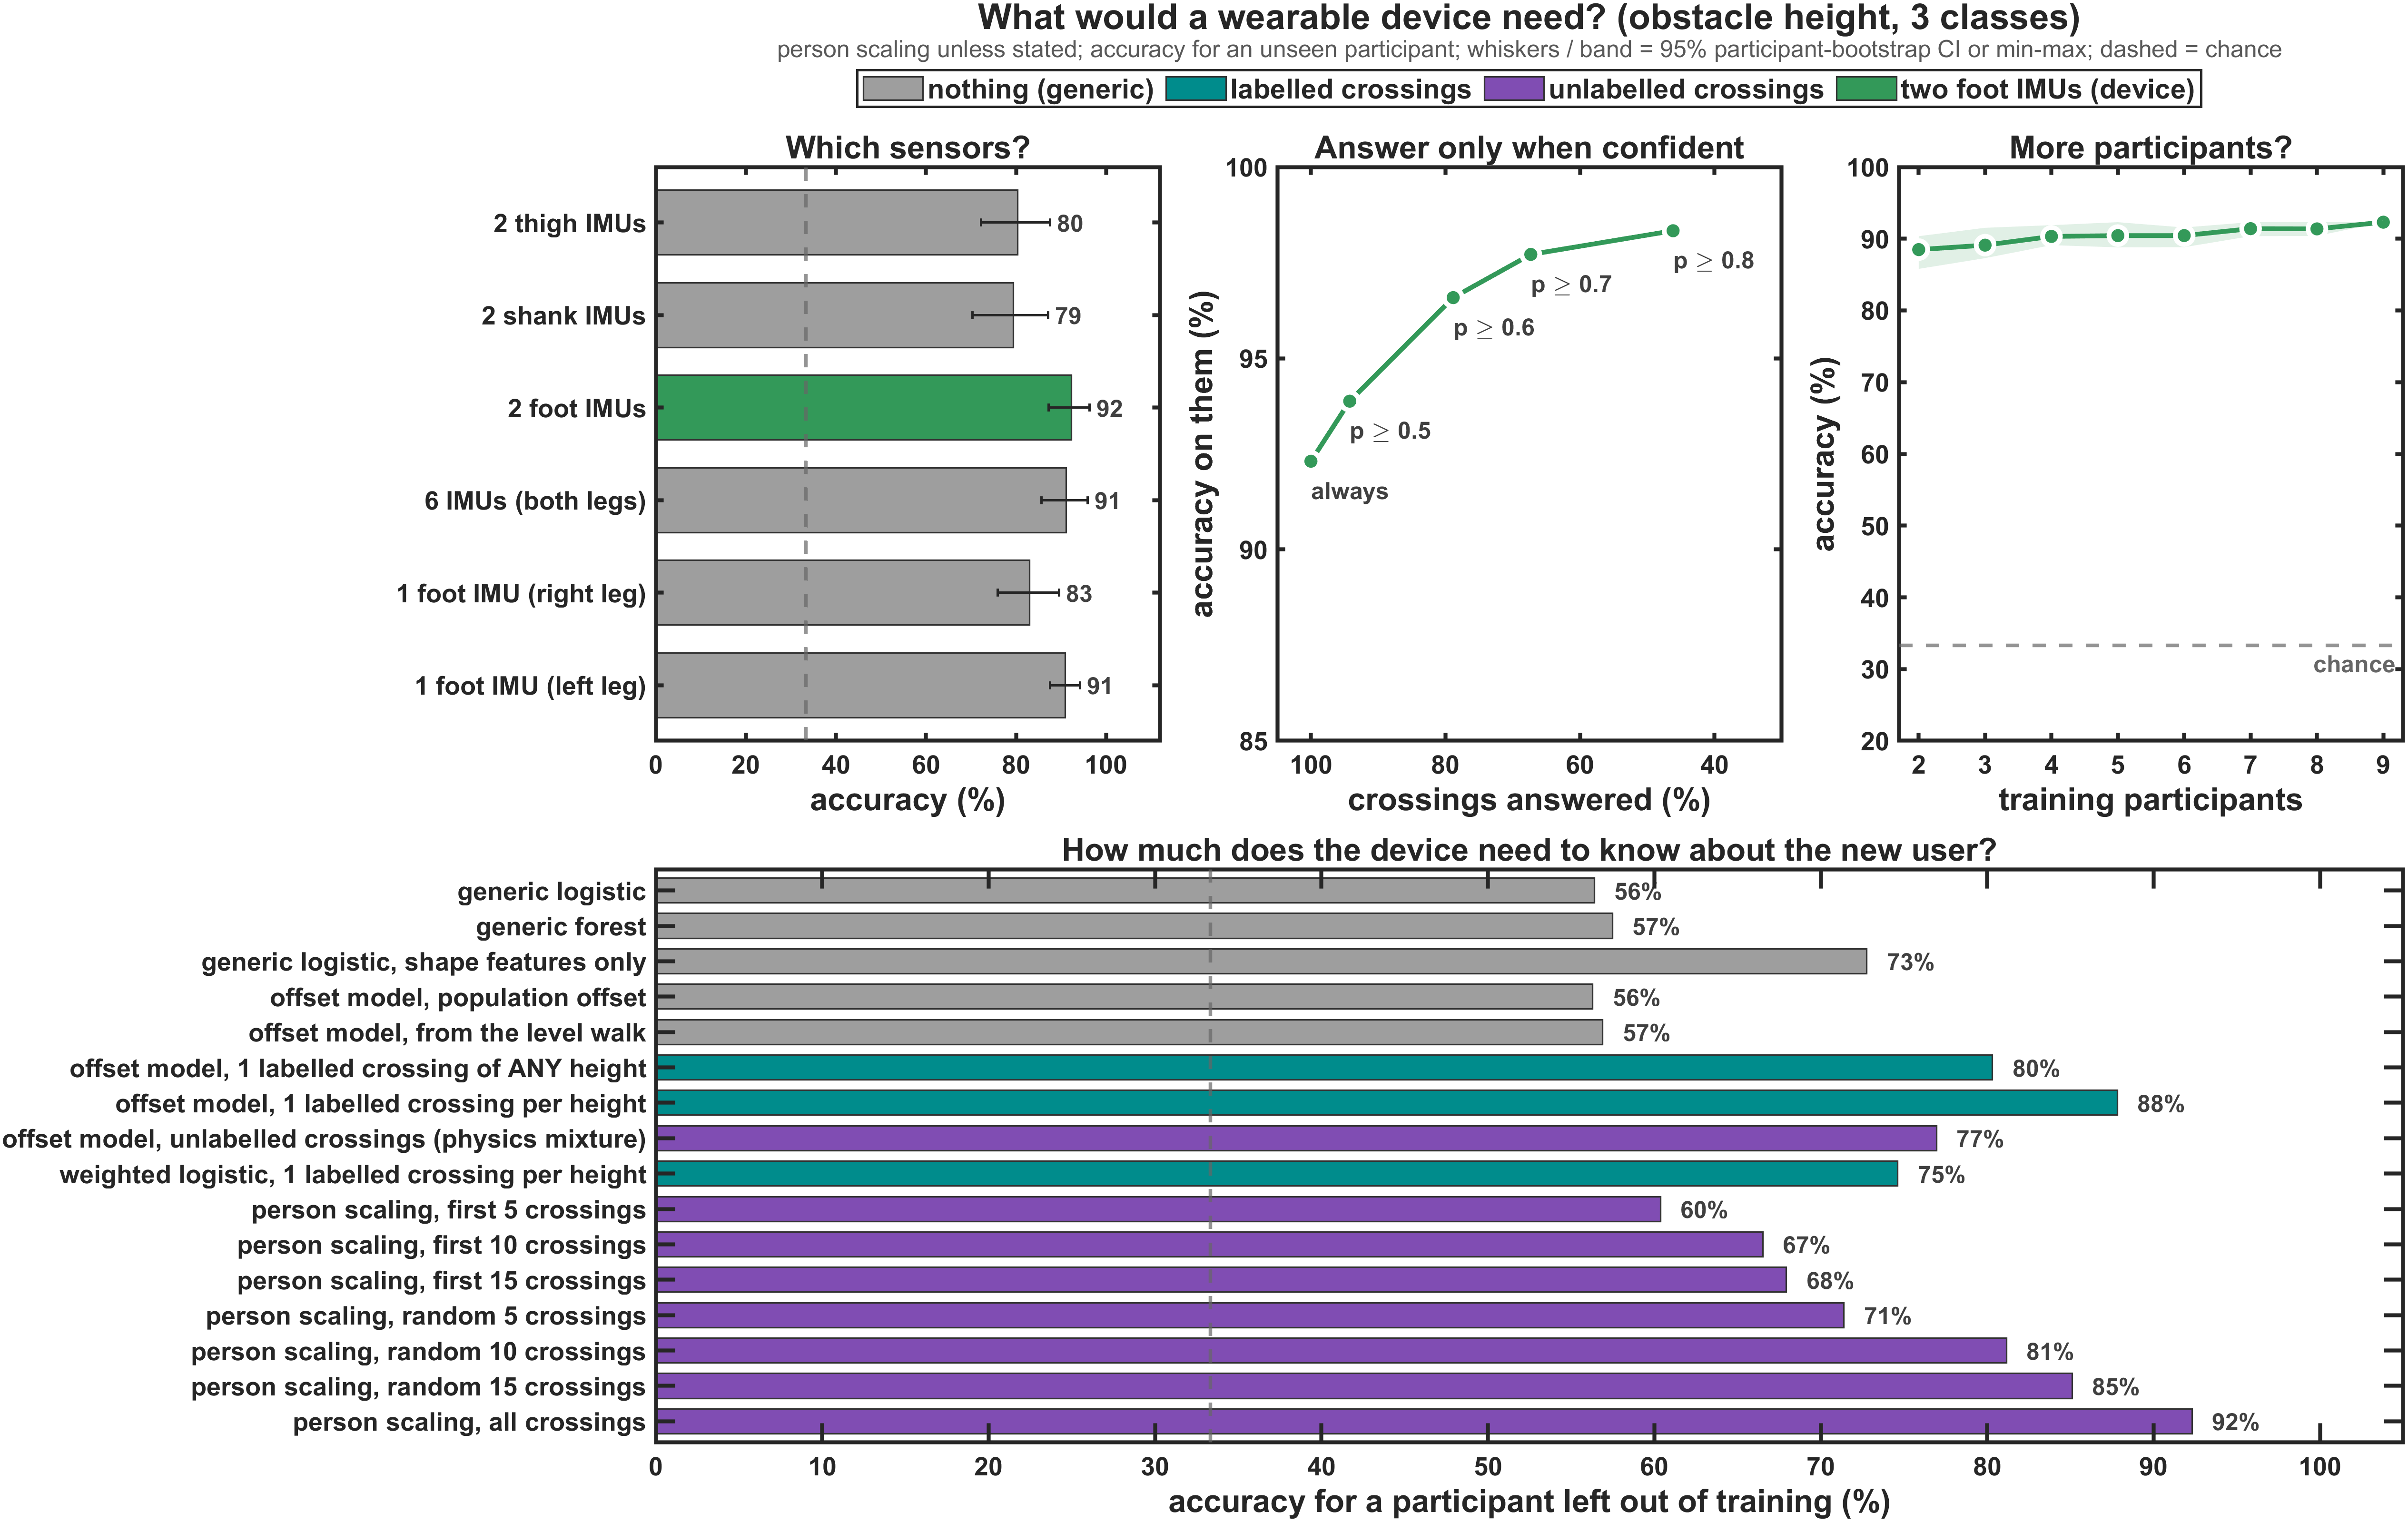
\includegraphics[width=\textwidth]{fig_device.png}
\caption{Device questions. Top: sensor sites (95\,\% CI; green = the two foot IMUs), accuracy against the share of crossings
answered when the device answers only above a probability threshold, and accuracy against the number of training participants
(band = min--max over the draws). Bottom: calibration options (grey = nothing about the new user, teal = labelled crossings,
purple = unlabelled crossings).}
\label{fig:device}
\end{figure}

\subsubsection{No camera: the end-to-end pipeline}

The pipeline that uses only the Dot (Table~\ref{tab:streamdetect}, Table~\ref{tab:streame2e}, Figure~\ref{fig:stream}) scans all
7250 strides of the sessions. It finds the obstacle-crossing strides with 98.7\,\% recall and 97.2\,\% precision, pairs them
into crossings with the right leading and trailing strides for 95.2\,\% of the crossings, and gives the right height for
90.7\,\% of the found crossings: 86.3\,\% of the crossings are fully correct (83.5\,\% when the 10 crossings without a valid
toe-off are counted as missed). Scaling the height features with the person's normal walking instead of their detected
crossings gives only 52.9\,\%: the personal scaling must come from crossings.

\begin{table}[htbp]
\centering
\caption{Finding the crossing strides among all strides of the session.}
\label{tab:streamdetect}
\begin{adjustbox}{max width=\textwidth}
{\footnotesize
\begin{tabular}{llrrr}
\toprule
\textbf{features} & \textbf{model} & \textbf{balanced accuracy} & \textbf{recall (crossings found)} & \textbf{precision (detections that are crossings)} \\
\midrule
raw & logistic & 93.8\% & 88.1\% & 94.8\% \\
raw & random forest & 99.2\% & 98.8\% & 95.9\% \\
scaled to own walking & logistic & 94.6\% & 89.6\% & 94.5\% \\
scaled to own walking & random forest & 99.2\% & 98.7\% & 97.2\% \\
\bottomrule
\end{tabular}
}
\end{adjustbox}

\end{table}

\begin{table}[htbp]
\centering
\caption{End to end: detect, pair (first foot = leading), classify the height.}
\label{tab:streame2e}
\begin{adjustbox}{max width=\textwidth}
{\footnotesize
\begin{tabular}{lrrrrr}
\toprule
\textbf{height scaling} & \textbf{crossings found} & \textbf{lead + trail strides right} & \textbf{height right (when found)} & \textbf{ALL correct} & \textbf{false crossings (per person)} \\
\midrule
crossing-scaled & 95.2\% & 95.2\% & 90.7\% & \textbf{86.3\%} & 1.4 \\
walking-scaled & 95.2\% & 95.2\% & 55.6\% & \textbf{52.9\%} & 1.4 \\
\bottomrule
\end{tabular}
}
\end{adjustbox}

\end{table}

\begin{figure}[htbp]
\centering
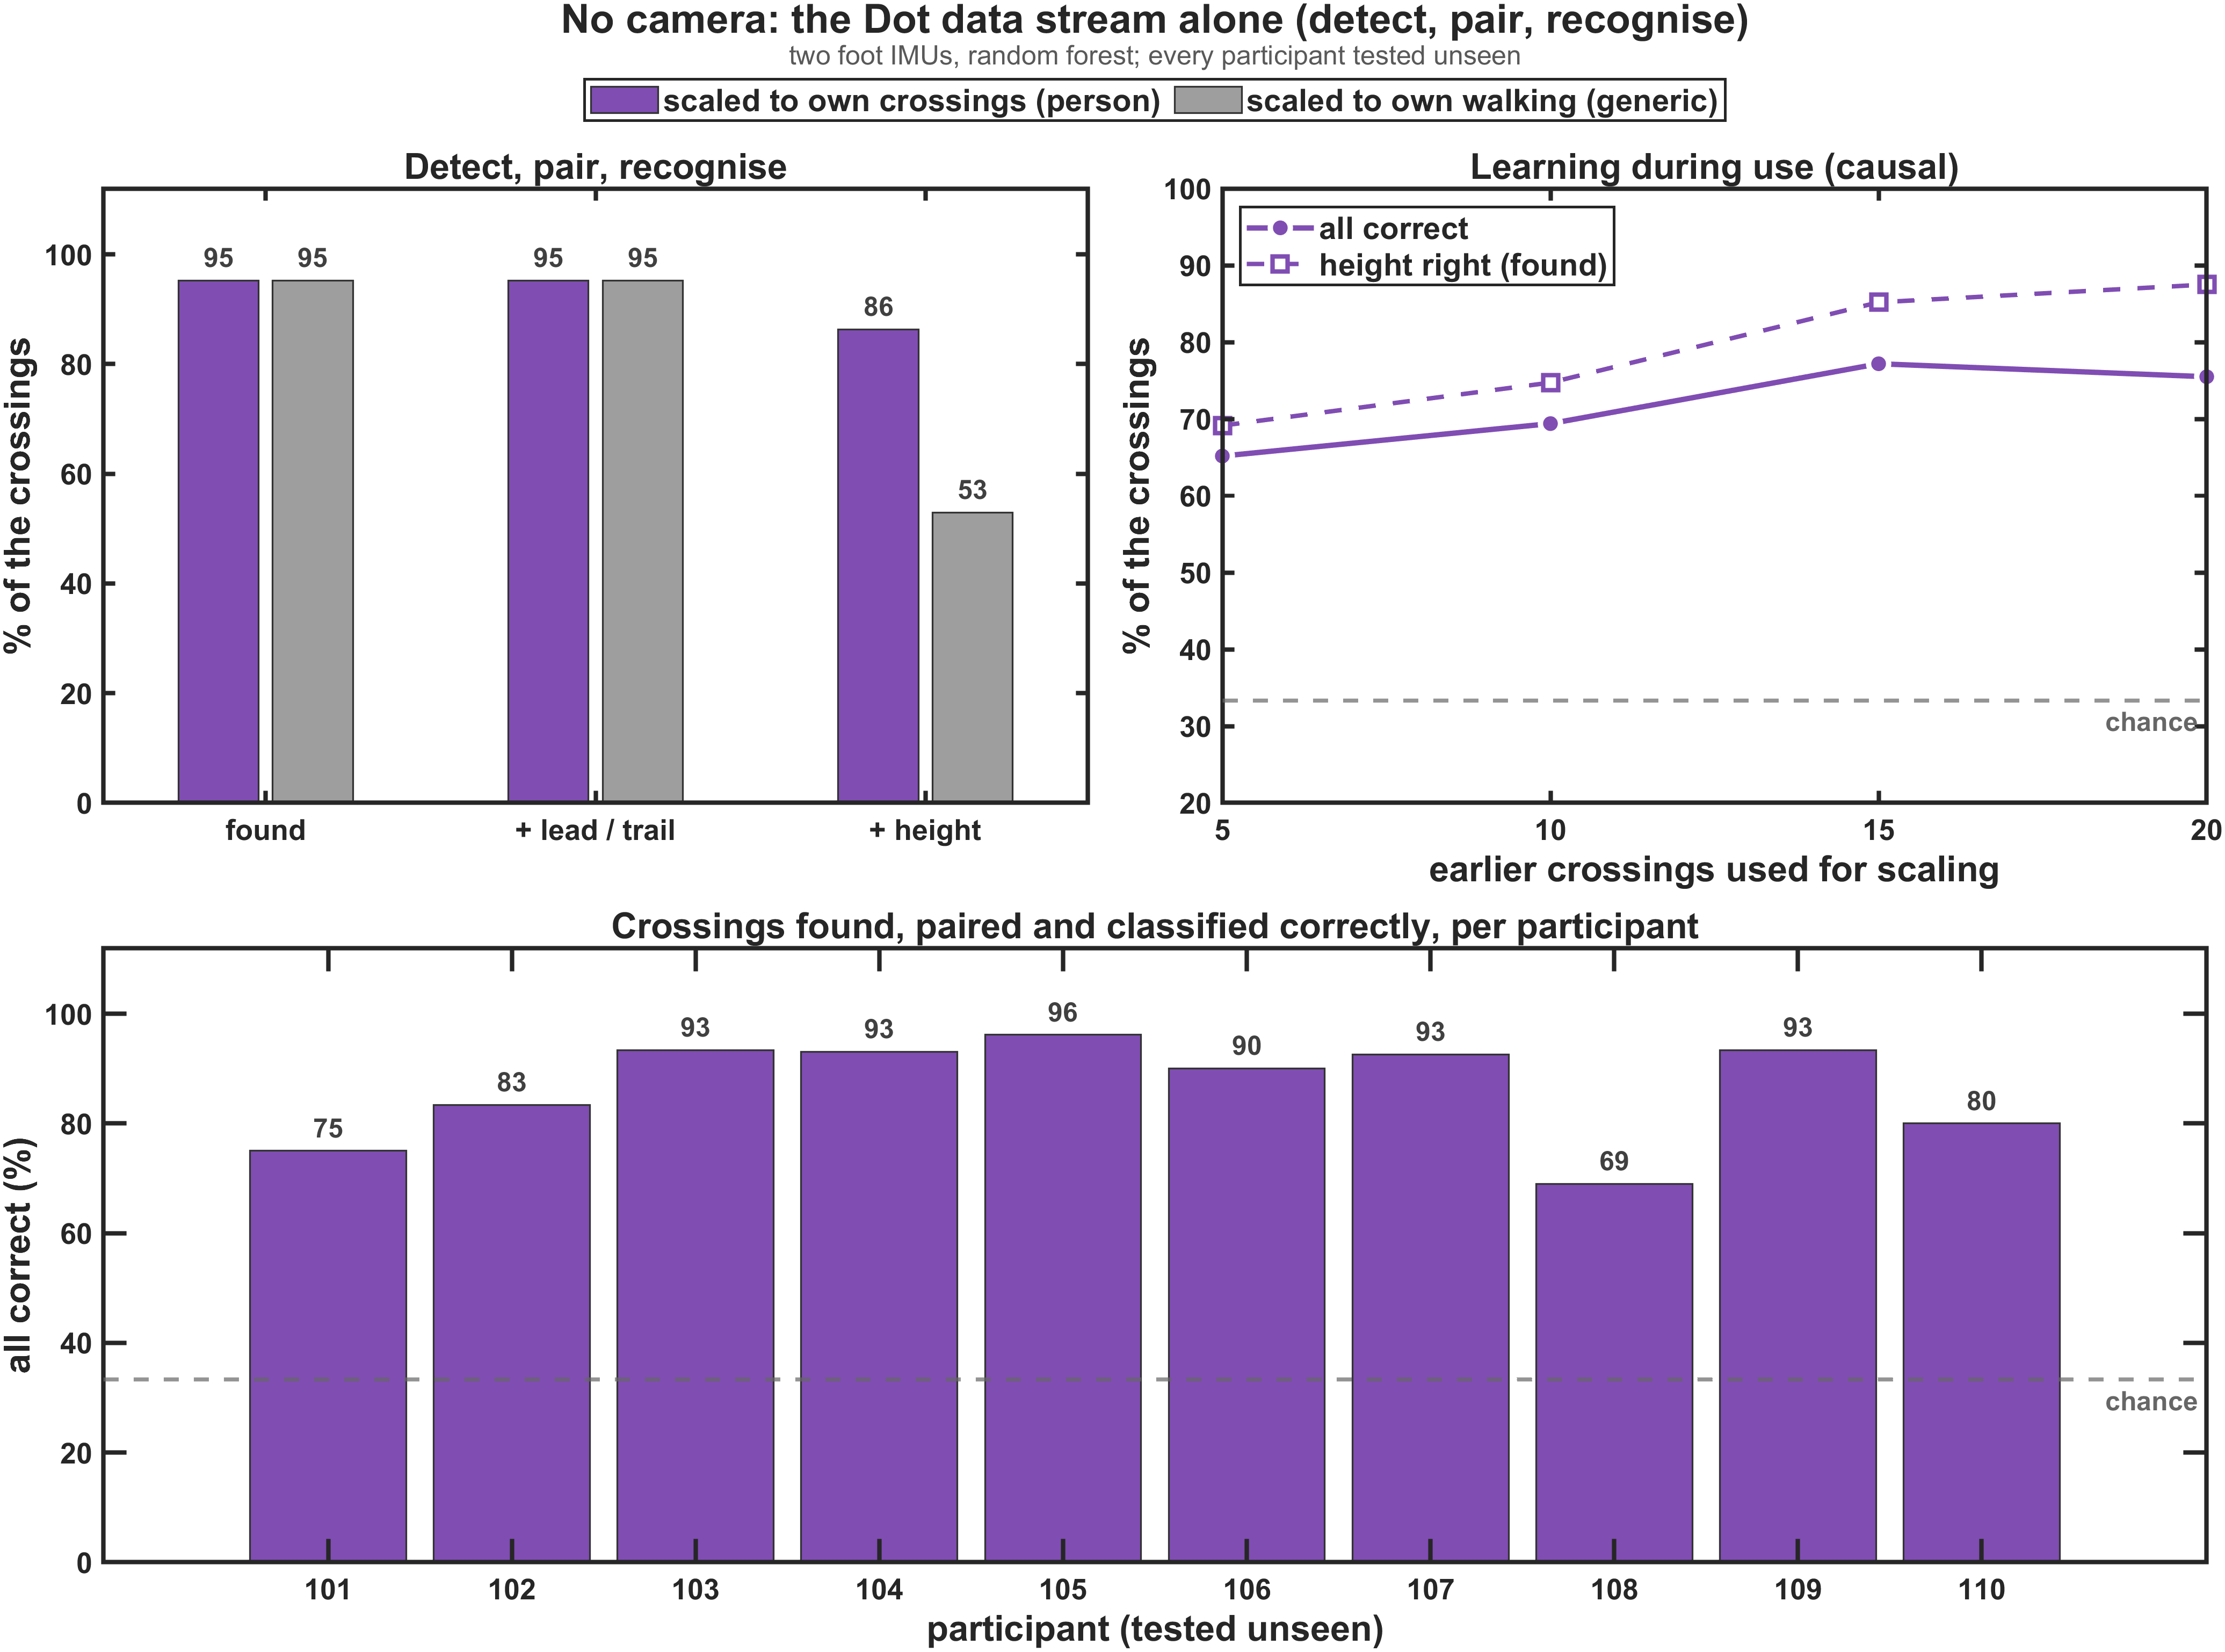
\includegraphics[width=\textwidth]{fig_stream.png}
\caption{Camera-free pipeline. Top left: share of the crossings found, also paired correctly (leading / trailing) and also
classified correctly, with the features scaled to the person's own crossings (purple) or own walking (grey). Top right: learning
during use (each crossing scaled with the earlier detected crossings only). Bottom: all-correct crossings per participant.}
\label{fig:stream}
\end{figure}

\subsubsection{A realistic session: obstacles in mixed order}
\label{sec:res-realworld}

The study ran the obstacles in blocks, but in daily life they come mixed. Each participant's crossings were shuffled 30 times and
the device worked causally: generic model for the first 5 (or 10) crossings, then person scaling learned from the crossings
already walked, without labels (Table~\ref{tab:mixed}, Figure~\ref{fig:realworld}). In mixed order the accuracy grows steadily
from 72\,\% (crossings 1--5) to 79\,\% (6--15) and 90\,\% from crossing 16 on. In the blocked study order the early history
covers only one or two obstacles, the person scaling is biased, and the accuracy collapses for crossings 6--15 before catching up.
The study's blocked-order ``learning during use'' numbers are therefore pessimistic for real use.

\begin{table}[htbp]
\centering
\caption{Accuracy by crossing number in a session, mixed (mean of 30 random orders) vs the real blocked order; generic model until
the switch, then causal person scaling.}
\label{tab:mixed}
\input{tables/realworld_mixed}
\end{table}

\subsubsection{A virtual real-time cue}
\label{sec:res-cue}

A real-time device must (a) notice the crossing and (b) decide the height while there is still time to cue the trailing limb.
(a) Over all 7250 strides of the sessions, online features available at the foot apex detect 99.0\,\% of the leading-limb
crossing strides, with about 3 false detections per session of about 725 strides. (b) The height is then predicted from the
leading-limb data available at the leading-foot apex (450\,ms before the trailing toe lift-off) or at its landing (200\,ms
before), with causal person scaling (Table~\ref{tab:cue}). In a mixed session about 71\,\% of the crossings get a correct cue at
the apex (76\,\% at landing); after 15 crossings 76\,\% (83\,\%). Answering only above a probability of 0.6 makes 79--82\,\% of
the given cues right but withholds 25--30\,\% of them. The real-time cue is less accurate than the after-the-fact recognition
(about 92\,\%) because only the leading limb has crossed when the cue must be sent.

\begin{table}[htbp]
\centering
\caption{Virtual real-time cue: outcome per crossing (correct / wrong / no cue), share of the given cues that are right, and the
correct cues after 15 crossings. Time left = median time to the trailing toe lift-off.}
\label{tab:cue}
\input{tables/realworld_cue}
\end{table}

\subsubsection{Why some participants are harder}

Once the device is scaled to the person, its errors follow how consistently that person lifts the \emph{trailing} foot for a given
height (Table~\ref{tab:dprime}): the person-scaled accuracy correlates with the trailing-foot separability $d'$ ($r = 0.77$,
leading $d'$: $r = 0.25$). The weakest participant (108, 73\,\%) has by far the least consistent trailing lift ($d' = 0.9$). The
generic model behaves differently ($r = -0.66$ with the trailing $d'$): its errors come from how far a person's personal margin
is from the group, which person scaling removes. With ten participants these correlations are indicative.

\begin{table}[htbp]
\centering
\caption{Per participant: separability of the heights in the leading and trailing foot lift ($d'$), the leading-foot lift SD within
a height and its slope, and the accuracy with person scaling and with the generic model.}
\label{tab:dprime}
\input{tables/realworld_dprime}
\end{table}

\begin{figure}[htbp]
\centering
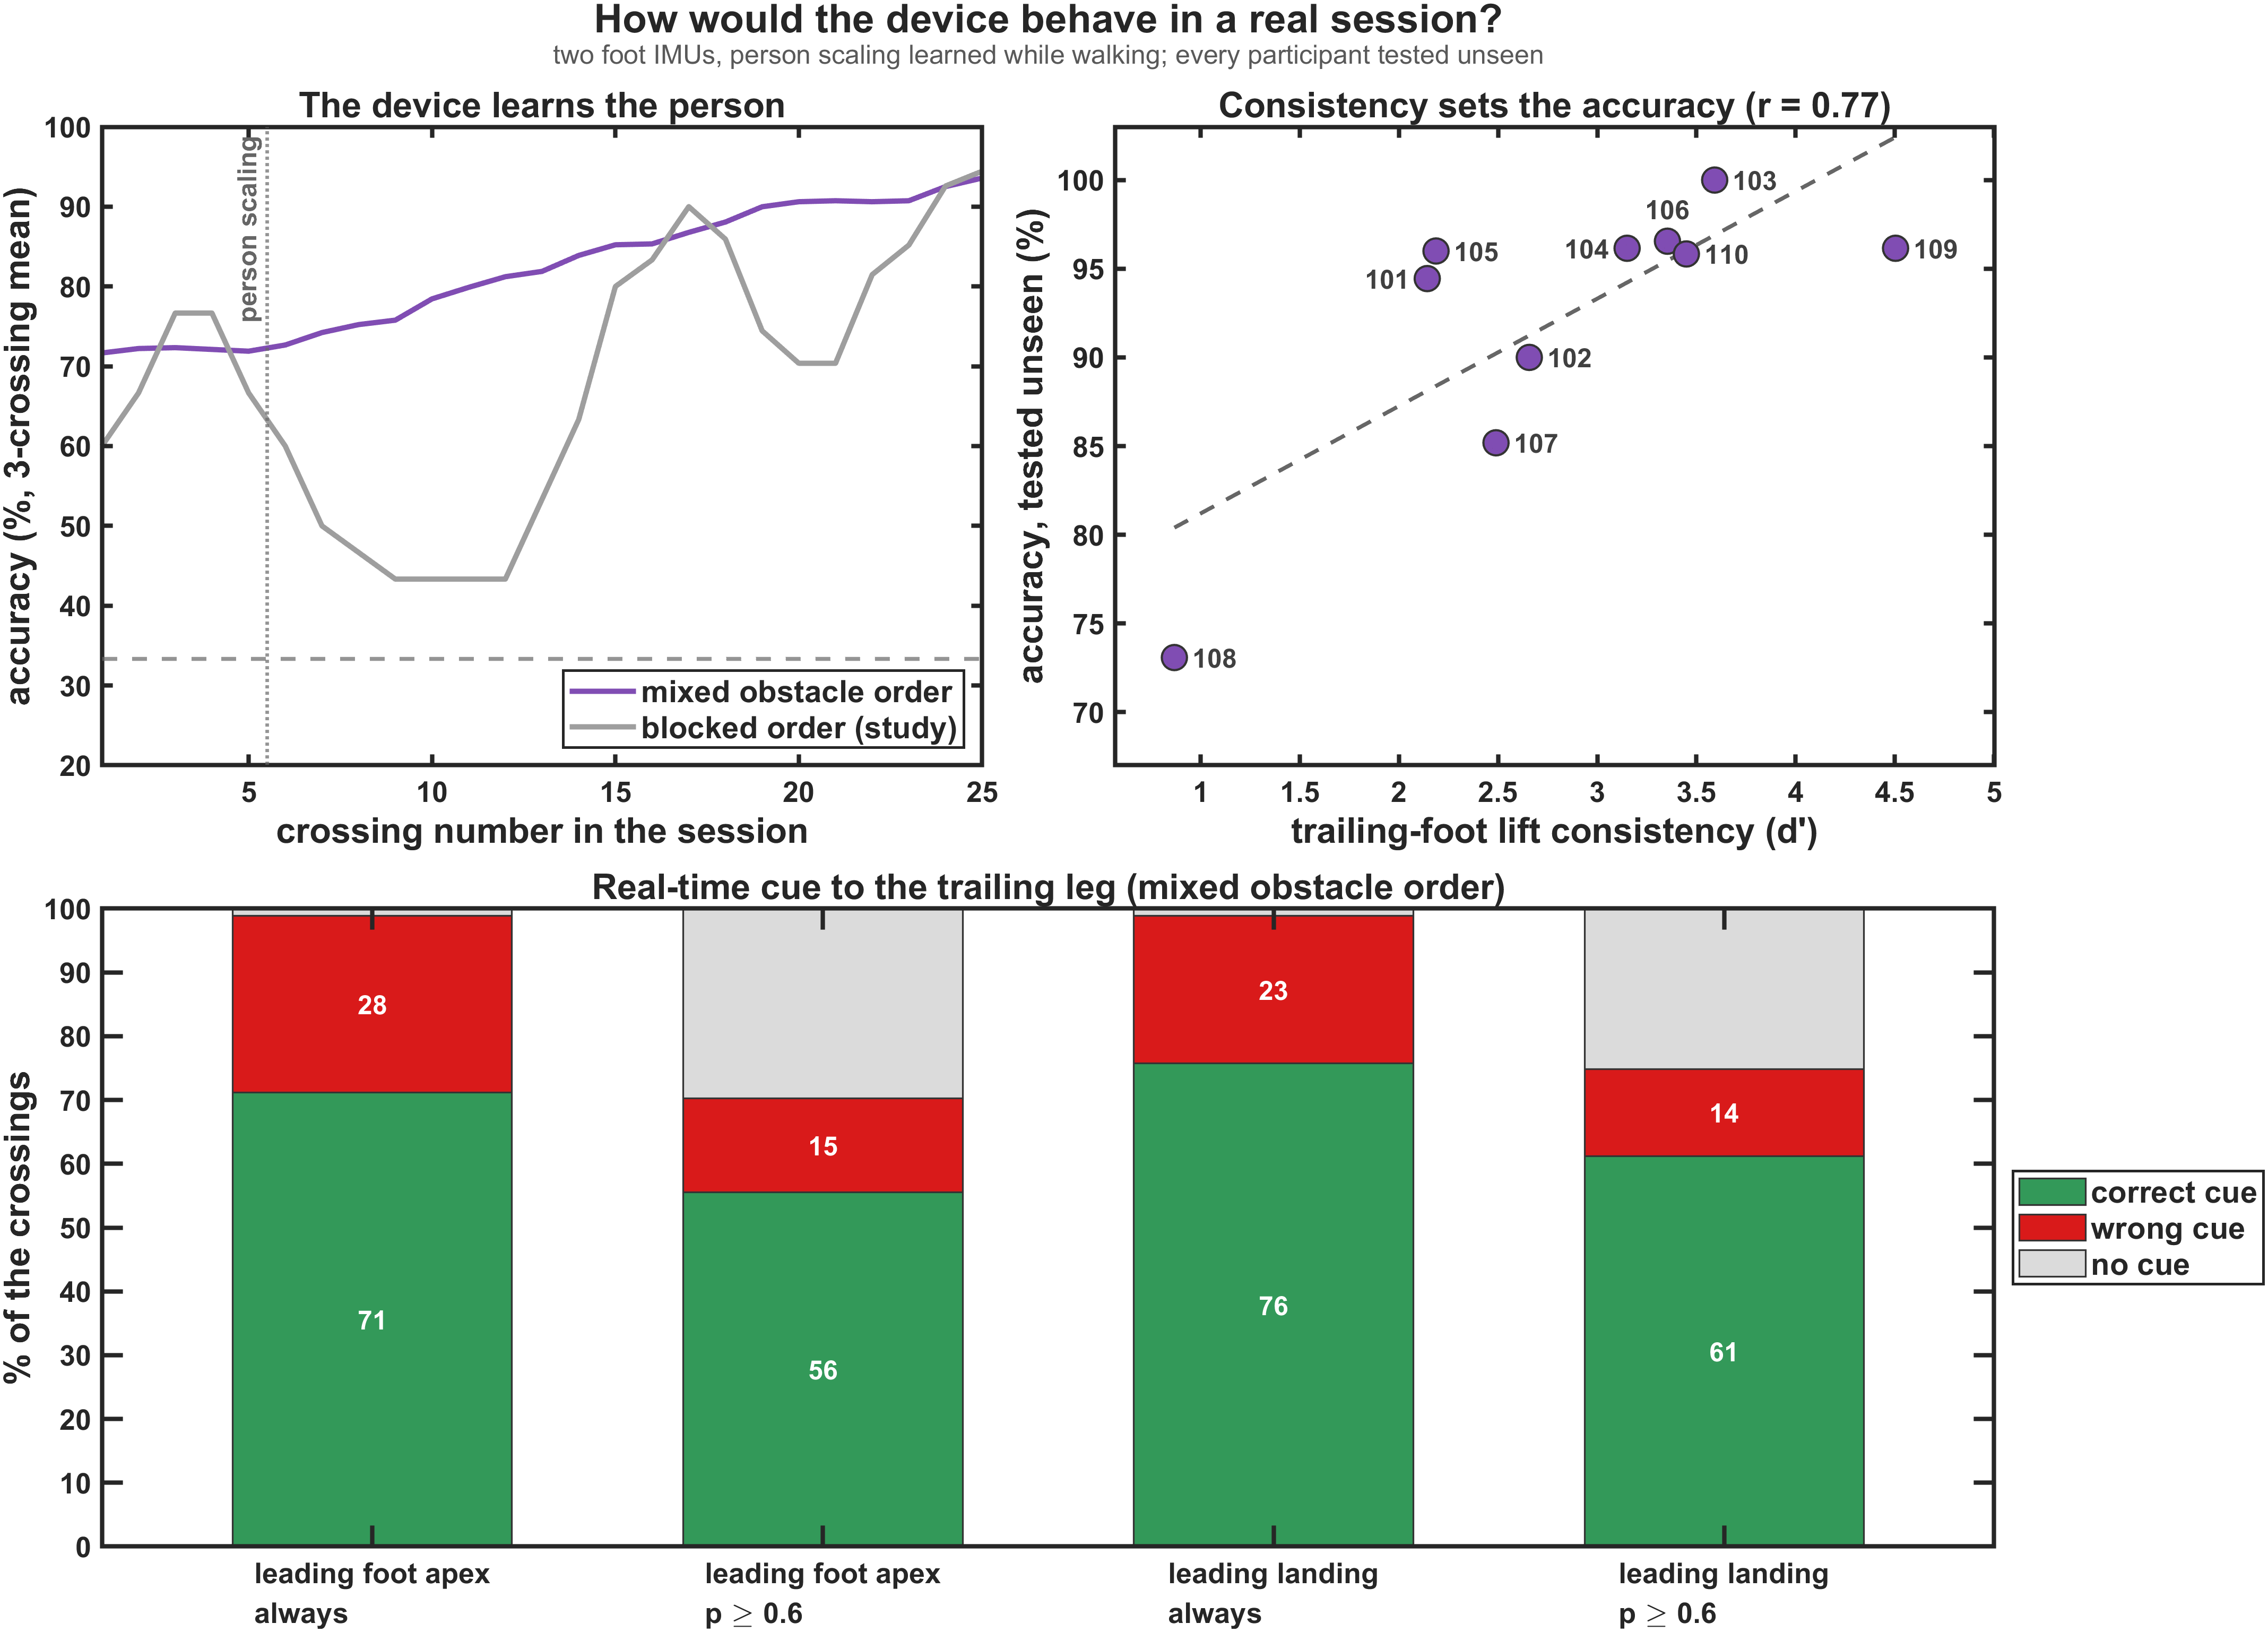
\includegraphics[width=\textwidth]{fig_realworld.png}
\caption{Real-world questions. Top left: accuracy by crossing number in a mixed vs blocked obstacle order (3-crossing moving
mean; dotted = start of person scaling; dashed = chance). Top right: person-scaled accuracy against the trailing-foot separability $d'$ per participant (dashed = least-squares line).
Bottom: outcome of the virtual real-time cue to the trailing leg for each cue moment and confidence threshold (green = correct,
red = wrong, grey = no cue).}
\label{fig:realworld}
\end{figure}


\subsection{Toe clearance}
\label{sec:res-clearance}

The camera minimum clearance (lowest toe or heel marker over the obstacle minus the obstacle top) is a safety outcome: a low
trailing clearance is a near-trip. With person-scaled Dot features the clearance is not predictable (Table~\ref{tab:safety}:
$r \approx 0$) and low-clearance crossings are only weakly detectable (AUC 0.63--0.73). The reason is that person scaling removes
each person's own margin, which is most of the clearance. Two further questions were therefore asked (Tables~\ref{tab:clearcells}
and \ref{tab:clearabs}): what sets the clearance from one crossing to the next, and how well the raw IMU foot lift predicts it.

\begin{table}[htbp]
\centering
\caption{Clearance from person-scaled Dot features (random forest): regression and detection of low-clearance crossings.}
\label{tab:safety}
\begin{adjustbox}{max width=\textwidth}
{\footnotesize
\begin{tabular}{p{4.6cm}p{4cm}p{6.2cm}}
\toprule
\textbf{task} & \textbf{inputs} & \textbf{result} \\
\midrule
regression of trail clearance (mm) & trail Dot features, self, forest & MAE 85 mm (predicting the mean: 84); r 0.04; within-person r median 0.28 \\
regression of lead clearance (mm) & lead Dot features, self, forest & MAE 49 mm (predicting the mean: 46); r $-$0.06; within-person r median 0.18 \\
regression of trail clearance (mm) & LEAD Dot features (cueing), self, forest & MAE 90 mm (predicting the mean: 84); r $-$0.14; within-person r median 0.08 \\
detect trailing clearance $\leq$ 0 mm (15 events) & trail Dot features, self, forest & AUC 0.73 \\
detect trailing clearance $\leq$ 30 mm (24 events) & trail Dot features, self, forest & AUC 0.70 \\
detect trailing clearance $\leq$ 50 mm (30 events) & trail Dot features, self, forest & AUC 0.63 \\
\bottomrule
\end{tabular}
}
\end{adjustbox}

\end{table}

\paragraph{What sets the clearance.} Within one participant and one obstacle the clearance still varies from crossing to crossing
(SD 37\,mm leading, 71\,mm trailing). About a third of this variation is explained by how high the toe goes (camera toe peak
above the obstacle: 35\,\% and 34\,\%), and very little by where the foot leaves the floor (take-off distance: 4\,\% and 6\,\%).
The IMU foot lift explains 20\,\% (leading) and 12\,\% (trailing): it follows the camera toe peak only partly ($r = 0.44$ and
0.21), because the sensor sits on the top of the foot and the trailing foot crosses heel-up, so the toe is not where the sensor
is. The provisional rigid-body toe estimate does no better.

\begin{table}[htbp]
\centering
\caption{What sets the crossing-to-crossing clearance (within participant $\times$ obstacle cells): SDs, correlations with the
clearance, and the share of the clearance variance explained.}
\label{tab:clearcells}
\begin{adjustbox}{max width=\textwidth}
{\footnotesize
\begin{tabular}{p{9.4cm}rr}
\toprule
\textbf{within participant x obstacle cells} & \textbf{leading limb} & \textbf{trailing limb} \\
\midrule
crossings (cells) & 260 (60) & 259 (60) \\
clearance SD (mm) & 37 & 71 \\
camera toe peak above the obstacle: SD (mm), r with clearance & 50, r = +0.59 & 84, r = +0.58 \\
camera take-off distance: SD (mm), r with clearance & 142, r = $-$0.19 & 89, r = +0.25 \\
IMU foot lift: SD (mm), r with clearance & 42, r = +0.44 & 37, r = +0.35 \\
IMU toe rise (provisional): SD (mm), r with clearance & 42, r = +0.43 & 34, r = +0.37 \\
r of IMU foot lift with the camera toe peak & +0.44 & +0.21 \\
r of IMU foot lift with the take-off distance & +0.05 & +0.01 \\
share of clearance variance explained: camera toe peak & 35\% & 34\% \\
share of clearance variance explained: camera take-off distance & 4\% & 6\% \\
share of clearance variance explained: camera toe peak + take-off & 37\% & 42\% \\
share of clearance variance explained: IMU foot lift & 20\% & 12\% \\
share of clearance variance explained: IMU toe rise (provisional) & 19\% & 13\% \\
share of clearance variance explained: IMU foot lift + take-off (camera) & 24\% & 18\% \\
\bottomrule
\end{tabular}
}
\end{adjustbox}

\end{table}

\paragraph{Absolute clearance for a new person.} Between people and obstacles the raw IMU foot lift (with the obstacle height) does
predict part of the clearance: mean absolute error 39\,mm for the leading and 65\,mm for the trailing limb, against 49 and 88\,mm for
the training mean (Table~\ref{tab:clearabs}). The camera's own toe peak would reach 34 and 55\,mm. Clearance is thus partly
predictable from the IMU; a trip-risk monitor needs a better toe-height estimate (a measured sensor-to-toe geometry).

\begin{table}[htbp]
\centering
\caption{Absolute clearance of a left-out participant (ordinary least squares): mean absolute error and correlation.}
\label{tab:clearabs}
\begin{adjustbox}{max width=\textwidth}
{\footnotesize
\begin{tabular}{lrr}
\toprule
\textbf{inputs} & \textbf{leading limb: MAE, r} & \textbf{trailing limb: MAE, r} \\
\midrule
constant (training mean) & 49 mm, r = $-$0.71 & 88 mm, r = $-$0.62 \\
IMU: foot lift + obstacle height & 39 mm, r = 0.49 & 65 mm, r = 0.56 \\
IMU + take-off distance (camera) & 42 mm, r = 0.40 & 66 mm, r = 0.55 \\
camera toe peak + take-off distance & 34 mm, r = 0.67 & 55 mm, r = 0.70 \\
\bottomrule
\end{tabular}
}
\end{adjustbox}

\end{table}

\subsection{A haptic cue: when, from which signal, with which threshold (Q4)}
\label{sec:res-haptic}

The cue is meant for the \emph{trailing} limb, which crosses the obstacle without seeing it. Its deadline is the moment the trailing
toe leaves the floor (camera lift-off); all times below are relative to that moment.

\subsubsection{Timeline of a crossing}

Table~\ref{tab:timeline} gives the median times. The leading toe leaves the floor 817\,ms before the deadline, the leading foot
reaches its apex at $-450$\,ms (IQR $-517$ to $-350$) and lands at $-200$\,ms (IQR $-300$ to $-33$). Once the trailing toe has left
the floor it is over the obstacle centre only 184\,ms later, too fast for any reaction. In 22\,\% of the crossings the trailing toe
even leaves the floor before the leading foot has landed (Table~\ref{tab:cueing}). The cue therefore has to come from the leading
limb, around its apex.

\begin{table}[htbp]
\centering
\caption{Timeline of a crossing relative to the trailing toe lift-off (deadline of a cue for the trailing limb).}
\label{tab:timeline}
\begin{adjustbox}{max width=\textwidth}
{\footnotesize
\begin{tabular}{p{7.4cm}rrr}
\toprule
\textbf{event} & \textbf{median (ms)} & \textbf{IQR (ms)} & \textbf{crossings} \\
\midrule
leading toe lift-off (camera) & $-$817 & $-$912 to $-$733 & 259 \\
leading toe-off event (IMU, step 4) & $-$733 & $-$817 to $-$621 & 259 \\
leading foot apex (IMU) & $-$450 & $-$517 to $-$350 & 259 \\
leading toe over the obstacle centre (camera) & $-$505 & $-$574 to $-$402 & 259 \\
leading heel-strike (landing, IMU) & $-$200 & $-$300 to $-$33 & 259 \\
trailing toe lift-off (camera) = deadline & +0 & +0 to +0 & 259 \\
trailing toe over the obstacle centre (camera) & +184 & +147 to +254 & 259 \\
trailing toe-off event (IMU, step 4) & +233 & +167 to +367 & 259 \\
trailing foot apex (IMU) & +300 & +233 to +433 & 259 \\
trailing heel-strike (landing, IMU) & +633 & +533 to +783 & 259 \\
\bottomrule
\end{tabular}
}
\end{adjustbox}

\end{table}

\begin{table}[htbp]
\centering
\caption{Cueing window: time from the leading-limb events to the trailing toe lift-off, overall and per height; \% $>$ 0 = share of
crossings in which the event comes before the lift-off.}
\label{tab:cueing}
\begin{adjustbox}{max width=\textwidth}
{\footnotesize
\begin{tabular}{lrrrrrrr}
\toprule
\textbf{interval} & \textbf{n} & \textbf{median} & \textbf{IQR} & \textbf{\% $>$ 0} & \textbf{H1 median} & \textbf{H2 median} & \textbf{H3 median} \\
\midrule
lead toe-off $\rightarrow$ trailing lift-off & 259 & 733 & 625 to 817 & 100\% & 658 & 783 & 800 \\
lead foot apex $\rightarrow$ trailing lift-off & 259 & 450 & 350 to 517 & 100\% & 383 & 483 & 450 \\
lead landing $\rightarrow$ trailing lift-off & 259 & 200 & 33 to 300 & 78\% & 133 & 233 & 200 \\
trailing lift-off $\rightarrow$ trailing foot apex & 259 & 300 & 233 to 433 & 100\% & 275 & 283 & 367 \\
trailing lift-off $\rightarrow$ step-4 trailing toe-off event (IMU) & 259 & 233 & 167 to 367 & 100\% & 200 & 217 & 317 \\
\bottomrule
\end{tabular}
}
\end{adjustbox}

\end{table}

\subsubsection{Detecting the crossing from one signal}

A single threshold on one leading-limb signal, referenced to the person's normal walking, detects the crossing early and reliably
(Table~\ref{tab:detect}): leading-thigh tilt more than 5.6\textdegree{} above normal walking at 30\,\% of the leading swing (573\,ms
before the deadline) gives 97\,\% sensitivity and 98\,\% specificity; leading-foot height more than 18.6\,mm above normal walking at
18\,\% of the swing (640\,ms before) gives 99\,\% and 98\,\%. Both reach at least 90\,\% sensitivity and specificity from 10\,\% and
4\,\% of the leading swing (682 and 713\,ms before the deadline). The leading shank and foot tilt are poor detectors. The trailing
limb detects equally well but only after its toe has left the floor. (Specificity is estimated on 39--46 level strides only; the
stride-based detector of Section~\ref{sec:res-cue}, tested on all 7250 strides, has about 3 false detections per session.)

\begin{table}[htbp]
\centering
\caption{Crossing vs level stride from one signal (vs normal walking): nested sensitivity / specificity, chosen moment and threshold,
and the earliest moment at which a fixed-moment rule reaches at least 90\,\% of both.}
\label{tab:detect}
\begin{adjustbox}{max width=\textwidth}
{\scriptsize
\begin{tabular}{llrrrr}
\toprule
\textbf{limb} & \textbf{signal} & \textbf{nested: sensitivity / specificity} & \textbf{moment chosen (median, \% swing; ms vs trailing lift-off)} & \textbf{threshold (vs normal walking)} & \textbf{earliest moment with both $\geq$ 90\%} \\
\midrule
lead & thigh tilt & 97\% / 98\% & 30\% ($-$573 ms) & $\geq$ +5.6 deg & 10\% ($-$682 ms) \\
lead & shank tilt & 61\% / 88\% & 14\% ($-$661 ms) & $\leq$ $-$3.0 deg & - \\
lead & foot tilt & 66\% / 88\% & 46\% ($-$479 ms) & $\geq$ +4.7 deg & - \\
lead & foot height & 99\% / 98\% & 18\% ($-$640 ms) & $\geq$ +18.6 mm & 4\% ($-$713 ms) \\
trail & thigh tilt & 93\% / 92\% & 46\% (+410 ms) & $\geq$ +4.3 deg & 32\% (+356 ms) \\
trail & shank tilt & 99\% / 98\% & 0\% (+233 ms) & $\leq$ $-$6.4 deg & 0\% (+233 ms) \\
trail & foot tilt & 95\% / 98\% & 14\% (+285 ms) & $\leq$ $-$7.7 deg & 0\% (+233 ms) \\
trail & foot height & 99\% / 98\% & 8\% (+261 ms) & $\geq$ +19.9 mm & 0\% (+233 ms) \\
\bottomrule
\end{tabular}
}
\end{adjustbox}

\end{table}

\subsubsection{Grading the height from one signal}

With two thresholds on one signal at one moment of the swing (Table~\ref{tab:grade}), the best leading-limb signal is the foot height
relative to the person's typical crossing: 73.4\,\% at 46\,\% of the leading swing (479\,ms before the deadline). The leading thigh
gives 63.9\,\% (72\,\% of the swing, 345\,ms before). Referenced only to normal walking (no crossing of the person yet) they give 45
and 52\,\%, because the personal margin is not removed. The leading shank and foot tilt do not grade the height. The trailing shank
(81.4\,\%) and trailing foot height (82.3\,\%) grade the height best, but only 250--300\,ms after the trailing toe has left the floor.
The multi-feature real-time model of Section~\ref{sec:res-cue} (71--76\,\% correct cues) is therefore comparable to the best single
leading-limb signal; the after-the-fact recognition with both limbs is much better (92\,\%).

\begin{table}[htbp]
\centering
\caption{Height from one signal at one moment of the swing (two ordered thresholds): nested accuracy, chosen moment and the device
thresholds (refitted on all participants).}
\label{tab:grade}
\begin{adjustbox}{max width=\textwidth}
{\scriptsize
\begin{tabular}{lllrrr}
\toprule
\textbf{limb} & \textbf{signal} & \textbf{reference} & \textbf{nested accuracy (95\% CI)} & \textbf{moment (\% swing; ms vs trailing lift-off)} & \textbf{thresholds H1/H2, H2/H3} \\
\midrule
lead & thigh tilt & vs normal walking & 52.4\% (40--64) & 42\% ($-$507 ms) & +43.3, +47.7 deg (rises with height) \\
lead & thigh tilt & person-centred & 63.9\% (52--74) & 72\% ($-$345 ms) & $-$3.2, +5.0 deg (rises with height) \\
lead & shank tilt & vs normal walking & 29.7\% (26--34) & 12\% ($-$671 ms) & $-$4.9, $-$10.4 deg (falls with height) \\
lead & shank tilt & person-centred & 38.9\% (30--47) & 48\% ($-$469 ms) & $-$5.0, +4.8 deg (rises with height) \\
lead & foot tilt & vs normal walking & 25.2\% (21--29) & 98\% ($-$210 ms) & +6.4, +3.8 deg (falls with height) \\
lead & foot tilt & person-centred & 43.2\% (37--49) & 48\% ($-$469 ms) & $-$4.7, +3.4 deg (rises with height) \\
lead & foot height & vs normal walking & 45.4\% (38--54) & 30\% ($-$573 ms) & +220.3, +295.2 mm (rises with height) \\
lead & foot height & person-centred & 73.4\% (62--82) & 46\% ($-$479 ms) & $-$35.8, +38.6 mm (rises with height) \\
trail & thigh tilt & vs normal walking & 36.3\% (34--40) & 50\% (+425 ms) & +18.4, +24.8 deg (rises with height) \\
trail & thigh tilt & person-centred & 35.0\% (26--44) & 42\% (+394 ms) & +1.4, +3.9 deg (rises with height) \\
trail & shank tilt & vs normal walking & 68.6\% (55--80) & 6\% (+254 ms) & $-$33.6, $-$46.2 deg (falls with height) \\
trail & shank tilt & person-centred & 81.4\% (72--89) & 6\% (+254 ms) & +6.5, $-$3.9 deg (falls with height) \\
trail & foot tilt & vs normal walking & 45.7\% (36--55) & 4\% (+247 ms) & $-$20.9, $-$26.9 deg (falls with height) \\
trail & foot tilt & person-centred & 60.2\% (51--67) & 4\% (+247 ms) & +4.1, $-$4.3 deg (falls with height) \\
trail & foot height & vs normal walking & 55.8\% (44--69) & 28\% (+341 ms) & +269.0, +352.6 mm (rises with height) \\
trail & foot height & person-centred & 82.3\% (74--89) & 16\% (+292 ms) & $-$46.6, +54.0 mm (rises with height) \\
\bottomrule
\end{tabular}
}
\end{adjustbox}

\end{table}

\subsubsection{How much: the extra angle and lift per height}

Table~\ref{tab:dose} gives, at the most informative moment of each signal, the mean value relative to normal walking for each height,
the change per cm of obstacle and the crossing-to-crossing SD. At 60\,\% of the leading swing (410\,ms before the deadline) the
leading thigh is flexed 35\textdegree{}, 46\textdegree{} and 53\textdegree{} more than in normal walking for H1, H2 and H3 (about
1\textdegree{} per cm, crossing-to-crossing SD 6.6\textdegree{}); the leading foot is 204, 298 and 361\,mm higher at its apex
(8.6\,mm per cm, SD 48\,mm). The trailing shank tilts backward 31\textdegree{}, 46\textdegree{} and 55\textdegree{} more at push-off
($-1.3$\textdegree{} per cm, SD 5.6\textdegree{}) and the trailing foot rises 237, 352 and 436\,mm (10.9\,mm per cm, SD 36\,mm). The
spread between participants (the $\pm$ values, 10--14\textdegree{} for the thigh, about 60--85\,mm for the foot height) is as large as the
step between two heights, so useful thresholds must be personal.

\begin{table}[htbp]
\centering
\caption{Extra angle and lift per height relative to normal walking (mean of the participant means $\pm$ SD across participants),
change per cm of obstacle, and crossing-to-crossing SD within a participant and obstacle.}
\label{tab:dose}
\begin{adjustbox}{max width=\textwidth}
{\scriptsize
\begin{tabular}{llrrrrrrr}
\toprule
\textbf{limb} & \textbf{signal} & \textbf{moment (\% swing; ms vs trailing lift-off)} & \textbf{$\eta^2$} & \textbf{H1} & \textbf{H2} & \textbf{H3} & \textbf{per cm of obstacle} & \textbf{crossing-to-crossing SD} \\
\midrule
lead & thigh tilt & 60\% ($-$410 ms) & 0.45 & +35.4 $\pm$ 9.9 & +45.8 $\pm$ 11.7 & +52.9 $\pm$ 13.5 & +0.95 deg & 6.6 deg \\
lead & shank tilt & 90\% ($-$248 ms) & 0.04 & $-$0.1 $\pm$ 7.9 & $-$3.2 $\pm$ 13.0 & $-$3.4 $\pm$ 12.9 & $-$0.15 deg & 5.8 deg \\
lead & foot tilt & 90\% ($-$248 ms) & 0.07 & +3.5 $\pm$ 11.1 & $-$0.7 $\pm$ 11.8 & $-$2.7 $\pm$ 11.6 & $-$0.29 deg & 6.4 deg \\
lead & foot height & 46\% ($-$479 ms) & 0.59 & +203.9 $\pm$ 65.5 & +297.6 $\pm$ 65.1 & +360.6 $\pm$ 75.9 & +8.62 mm & 47.6 mm \\
trail & thigh tilt & 44\% (+402 ms) & 0.14 & +13.4 $\pm$ 4.6 & +16.3 $\pm$ 7.0 & +18.4 $\pm$ 8.5 & +0.28 deg & 3.9 deg \\
trail & shank tilt & 4\% (+247 ms) & 0.65 & $-$31.1 $\pm$ 14.1 & $-$45.6 $\pm$ 13.5 & $-$54.7 $\pm$ 9.3 & $-$1.30 deg & 5.6 deg \\
trail & foot tilt & 2\% (+240 ms) & 0.35 & $-$18.1 $\pm$ 11.6 & $-$28.1 $\pm$ 12.0 & $-$33.7 $\pm$ 10.6 & $-$0.85 deg & 7.4 deg \\
trail & foot height & 18\% (+299 ms) & 0.75 & +237.4 $\pm$ 84.4 & +352.3 $\pm$ 70.5 & +436.0 $\pm$ 59.2 & +10.89 mm & 36.1 mm \\
\bottomrule
\end{tabular}
}
\end{adjustbox}

\end{table}

\subsubsection{Real time: fixed times before the deadline}

On the time-aligned signals (Table~\ref{tab:realtime}, Figure~\ref{fig:haptic}), the leading foot height is again the best single
signal (person-centred 72\,\%, best about 470\,ms before the deadline), and the leading thigh gives about 60\,\%. Every trailing-limb
signal stays near chance (41--51\,\%) before the lift-off: the trailing limb shows no sign of the obstacle height before it leaves the
floor. Fixed clock times blur the signals, because the timing of the crossing varies from one crossing to the next; a device should
trigger on leading-limb events (toe-off, apex) rather than on a fixed clock. Table~\ref{tab:rules} lists the corresponding rules
referenced to normal walking for a cue that must be ready 300\,ms before the deadline.

\begin{table}[htbp]
\centering
\caption{Height from one signal at fixed times before the trailing toe lift-off: nested accuracy for each cue deadline (median chosen
time in brackets).}
\label{tab:realtime}
\begin{adjustbox}{max width=\textwidth}
{\scriptsize
\begin{tabular}{lllrrrrr}
\toprule
\textbf{limb} & \textbf{signal} & \textbf{reference} & \textbf{data up to 500 ms before} & \textbf{data up to 300 ms before} & \textbf{data up to 200 ms before} & \textbf{data up to 100 ms before} & \textbf{up to the lift-off} \\
\midrule
lead & thigh tilt & vs normal walking & 39\% ($-$500 ms) & 55\% ($-$417 ms) & 55\% ($-$417 ms) & 55\% ($-$417 ms) & 55\% ($-$417 ms) \\
lead & thigh tilt & person-centred & 61\% ($-$500 ms) & 60\% ($-$417 ms) & 60\% ($-$417 ms) & 60\% ($-$417 ms) & 60\% ($-$417 ms) \\
lead & shank tilt & vs normal walking & 33\% ($-$967 ms) & 33\% ($-$967 ms) & 33\% ($-$967 ms) & 33\% ($-$967 ms) & 33\% ($-$967 ms) \\
lead & shank tilt & person-centred & 49\% ($-$817 ms) & 49\% ($-$817 ms) & 49\% ($-$817 ms) & 49\% ($-$817 ms) & 49\% ($-$817 ms) \\
lead & foot tilt & vs normal walking & 39\% ($-$900 ms) & 39\% ($-$900 ms) & 39\% ($-$900 ms) & 39\% ($-$900 ms) & 39\% ($-$900 ms) \\
lead & foot tilt & person-centred & 38\% ($-$950 ms) & 38\% ($-$950 ms) & 38\% ($-$950 ms) & 38\% ($-$950 ms) & 38\% ($-$950 ms) \\
lead & foot height & vs normal walking & 49\% ($-$500 ms) & 54\% ($-$450 ms) & 54\% ($-$450 ms) & 54\% ($-$450 ms) & 54\% ($-$450 ms) \\
lead & foot height & person-centred & 72\% ($-$500 ms) & 72\% ($-$467 ms) & 72\% ($-$467 ms) & 72\% ($-$467 ms) & 72\% ($-$467 ms) \\
trail & thigh tilt & vs normal walking & 41\% ($-$1333 ms) & 41\% ($-$1333 ms) & 41\% ($-$1333 ms) & 41\% ($-$1333 ms) & 41\% ($-$1333 ms) \\
trail & thigh tilt & person-centred & 51\% ($-$1217 ms) & 51\% ($-$1217 ms) & 51\% ($-$1217 ms) & 51\% ($-$1217 ms) & 51\% ($-$1217 ms) \\
trail & shank tilt & vs normal walking & 43\% ($-$1500 ms) & 43\% ($-$1500 ms) & 43\% ($-$1500 ms) & 43\% ($-$1500 ms) & 43\% ($-$1500 ms) \\
trail & shank tilt & person-centred & 42\% ($-$1475 ms) & 42\% ($-$1475 ms) & 42\% ($-$1475 ms) & 42\% ($-$1475 ms) & 42\% ($-$1475 ms) \\
trail & foot tilt & vs normal walking & 41\% ($-$1450 ms) & 41\% ($-$1450 ms) & 41\% ($-$1450 ms) & 41\% ($-$1450 ms) & 41\% ($-$1450 ms) \\
trail & foot tilt & person-centred & 46\% ($-$1467 ms) & 46\% ($-$1467 ms) & 46\% ($-$1467 ms) & 46\% ($-$1467 ms) & 46\% ($-$1467 ms) \\
trail & foot height & vs normal walking & 43\% ($-$1417 ms) & 43\% ($-$1417 ms) & 43\% ($-$1417 ms) & 43\% ($-$1417 ms) & 43\% ($-$1417 ms) \\
trail & foot height & person-centred & 50\% ($-$1383 ms) & 50\% ($-$1383 ms) & 50\% ($-$1383 ms) & 50\% ($-$1383 ms) & 50\% ($-$1383 ms) \\
\bottomrule
\end{tabular}
}
\end{adjustbox}

\end{table}

\begin{table}[htbp]
\centering
\caption{Single-signal rules for a cue ready 300\,ms before the trailing toe lift-off (referenced to normal walking; refitted on all
participants).}
\label{tab:rules}
\begin{adjustbox}{max width=\textwidth}
{\scriptsize
\begin{tabular}{llrrrlr}
\toprule
\textbf{limb} & \textbf{signal} & \textbf{moment (ms vs lift-off)} & \textbf{H1/H2 threshold} & \textbf{H2/H3 threshold} & \textbf{direction} & \textbf{accuracy on left-out participants} \\
\midrule
lead & thigh tilt & $-$417 & +34.4 deg & +45.5 deg & higher obstacle = larger value & 55\% \\
lead & shank tilt & $-$1133 & +0.9 deg & $-$10.6 deg & higher obstacle = smaller value & 33\% \\
lead & foot tilt & $-$850 & $-$23.5 deg & $-$44.1 deg & higher obstacle = smaller value & 39\% \\
lead & foot height & $-$450 & +230.8 mm & +325.4 mm & higher obstacle = larger value & 54\% \\
trail & thigh tilt & $-$1333 & +15.9 deg & +31.3 deg & higher obstacle = larger value & 41\% \\
trail & shank tilt & $-$1500 & $-$4.3 deg & $-$26.3 deg & higher obstacle = smaller value & 43\% \\
trail & foot tilt & $-$1450 & $-$4.8 deg & $-$46.2 deg & higher obstacle = smaller value & 41\% \\
trail & foot height & $-$1433 & +7.5 mm & +21.1 mm & higher obstacle = larger value & 43\% \\
\bottomrule
\end{tabular}
}
\end{adjustbox}

\end{table}

Figure~\ref{fig:haptic} shows the accuracy of one signal over time and Figure~\ref{fig:hapticcurves} the signals behind it: the
leading thigh tilt and foot height separate the three heights from about 0.6--0.8\,s before the trailing toe lift-off, whereas the
trailing shank and foot separate them only after it.

\begin{figure}[htbp]
\centering
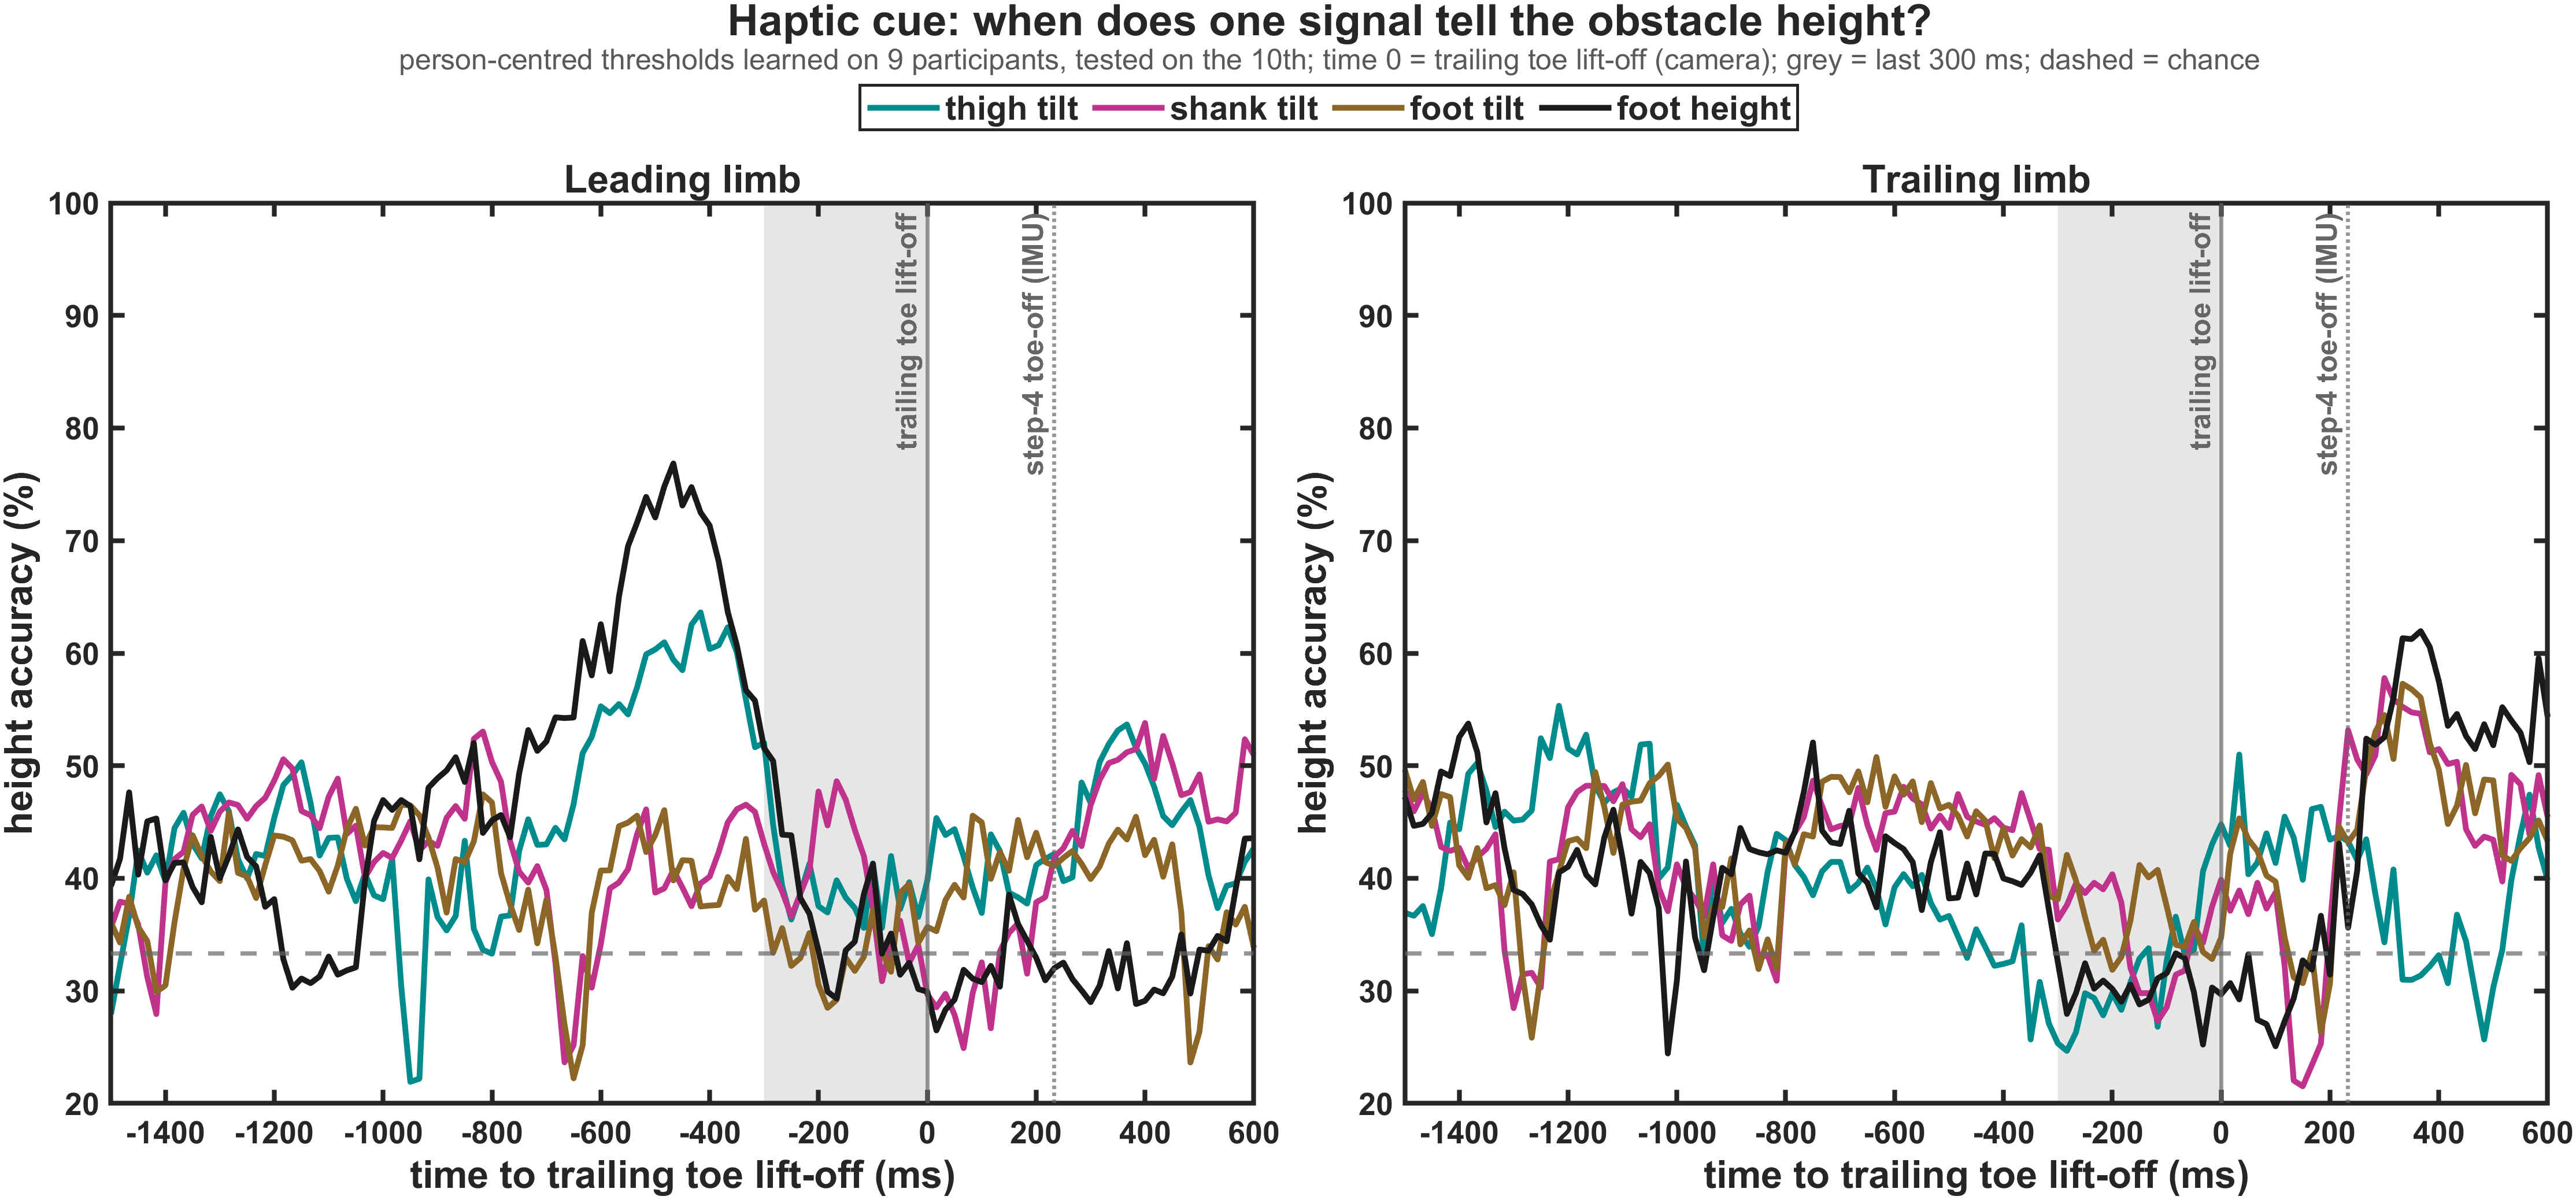
\includegraphics[width=\textwidth]{fig_haptic.png}
\caption{Haptic timing: height accuracy from one signal with person-centred thresholds (learned on nine participants, tested on the
tenth) at each time relative to the trailing toe lift-off, for the leading (left) and the trailing (right) limb. Grey = last 300\,ms;
dotted = median step-4 trailing toe-off event (IMU); dashed = chance.}
\label{fig:haptic}
\end{figure}

\begin{figure}[htbp]
\centering
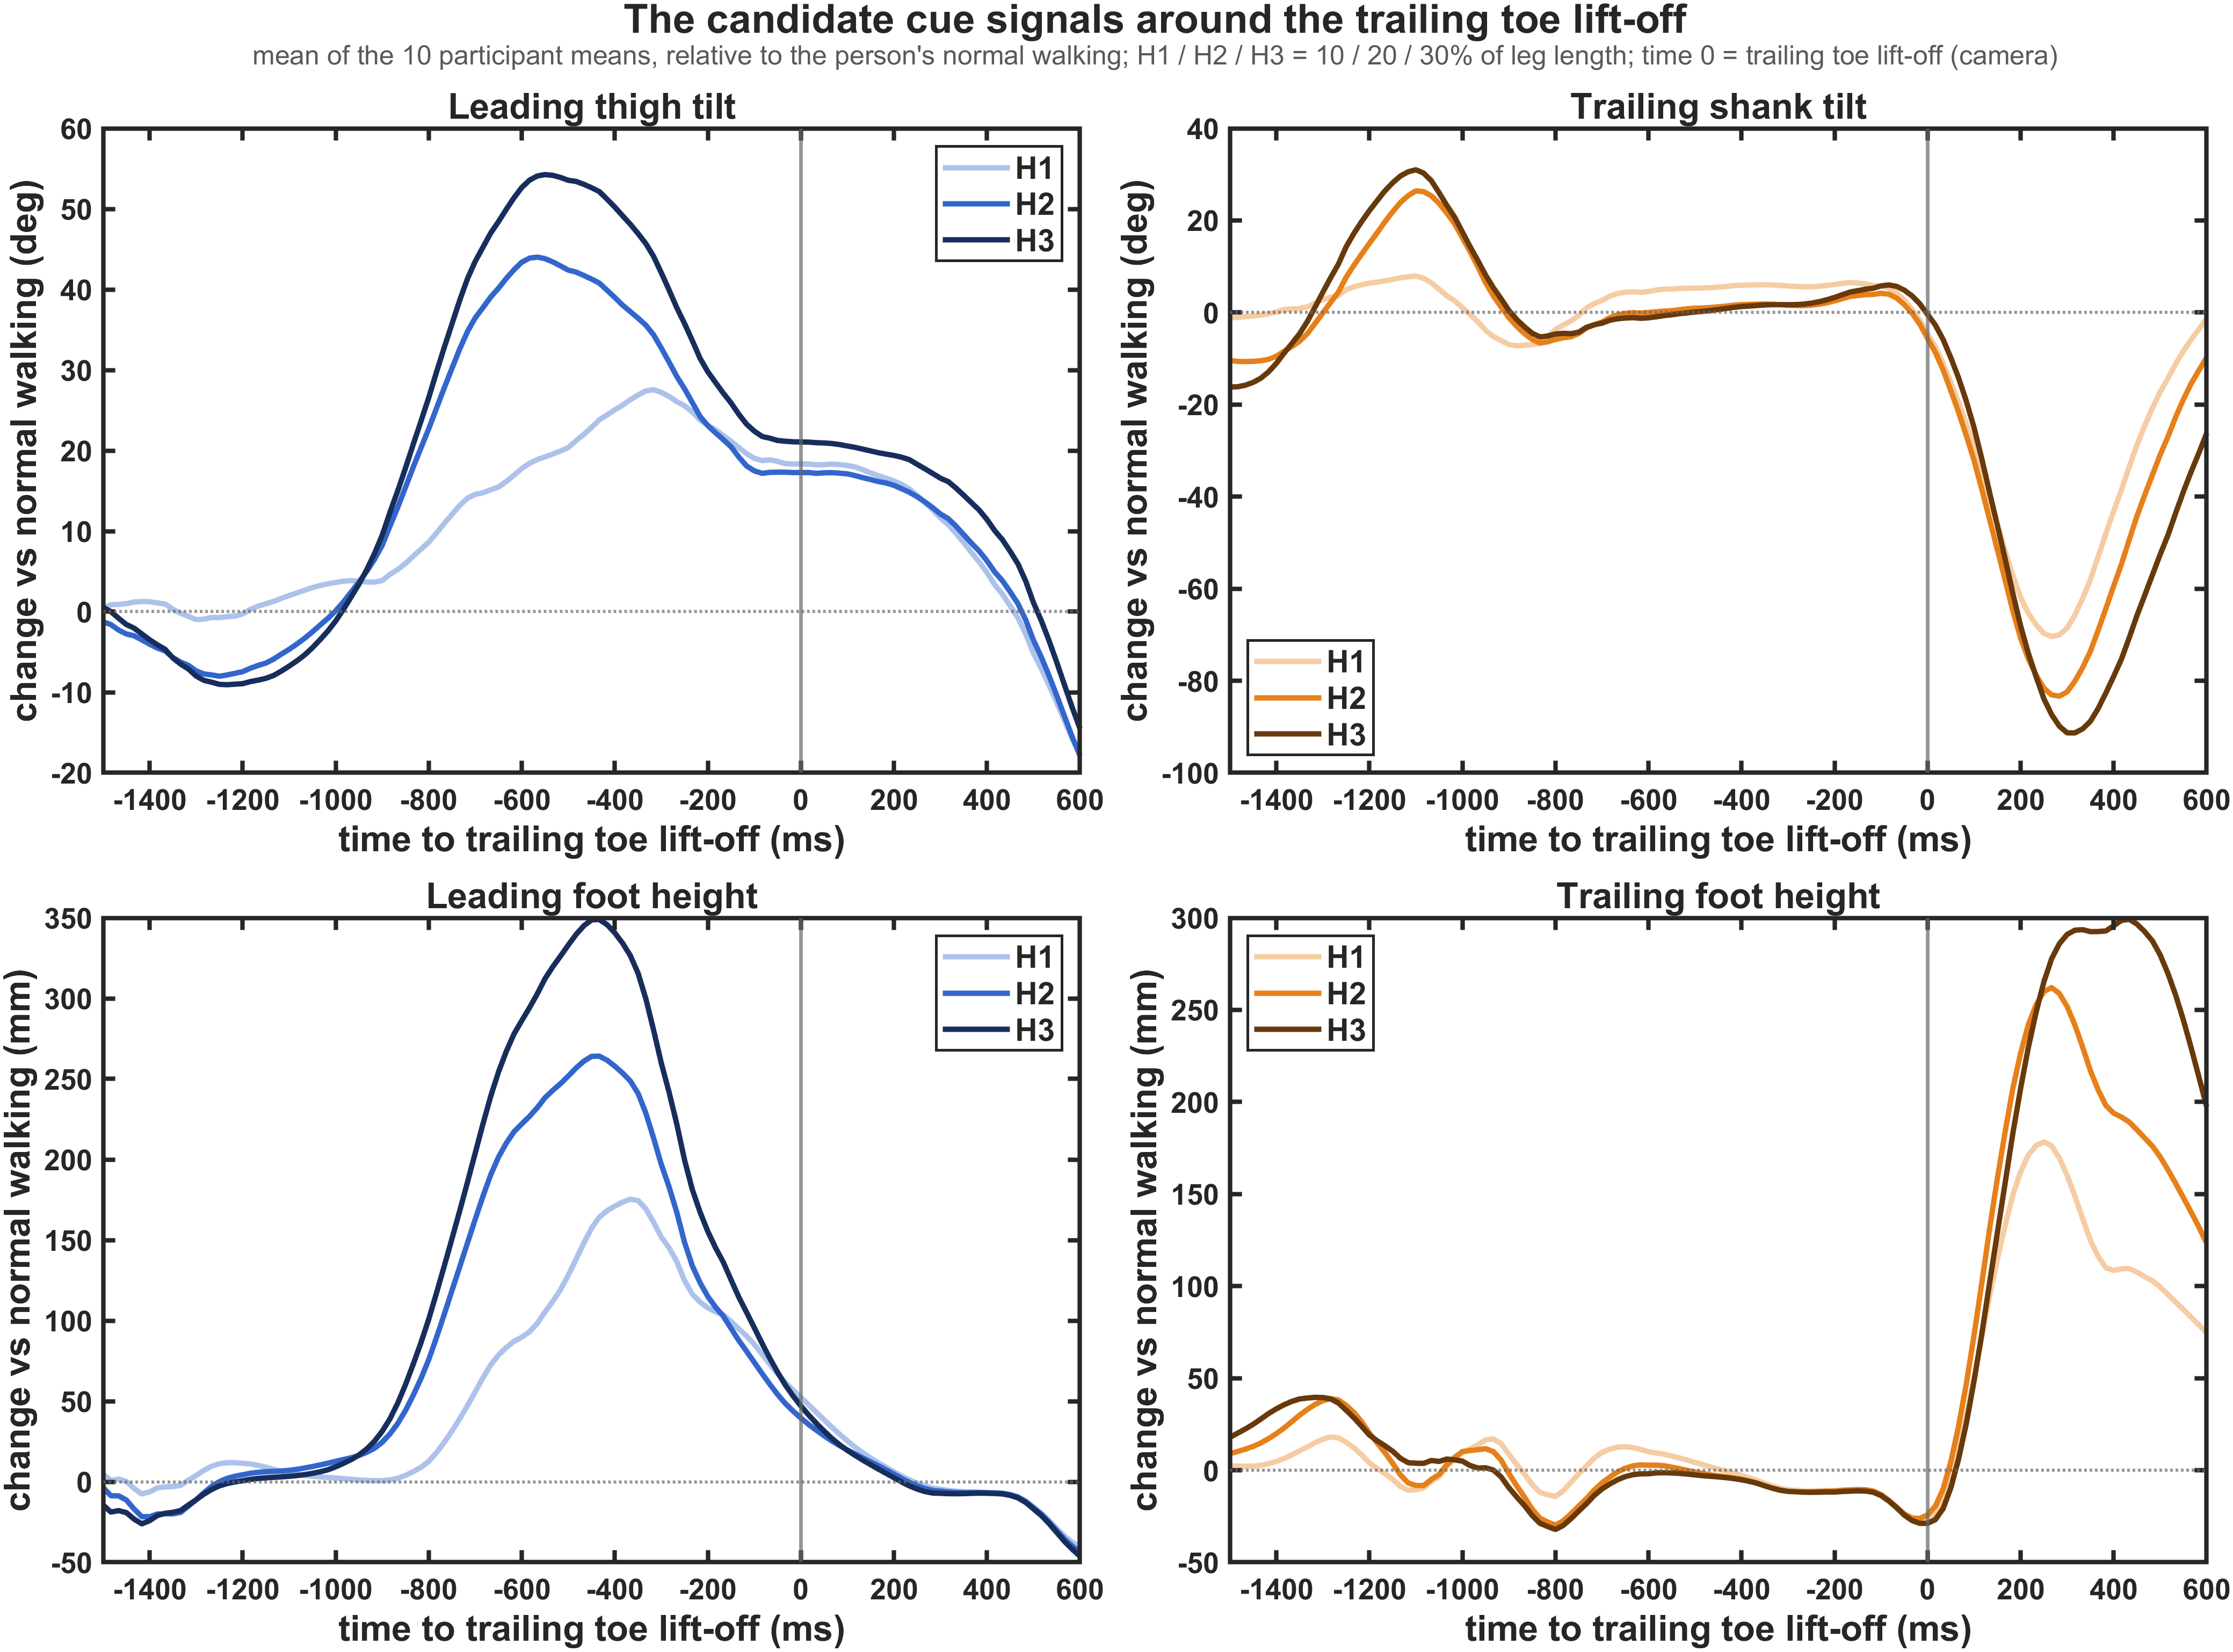
\includegraphics[width=\textwidth]{fig_haptic_curves.png}
\caption{The candidate cue signals around the trailing toe lift-off, relative to the person's normal walking: leading thigh tilt,
trailing shank tilt, leading and trailing foot height. Mean of the 10 participant means per obstacle height (light to dark =
H1 to H3); vertical line = trailing toe lift-off.}
\label{fig:hapticcurves}
\end{figure}


\section{Interpretation and recommendations}
\label{sec:discussion}

\subsection{What the results mean}

\paragraph{A simple physical rule, a strong personal component.} Young adults clear an obstacle by lifting each foot by about the
obstacle height (about 10\,mm per cm) while keeping their safety margin, mainly through leading-thigh flexion and trailing heel-up.
On top of this rule every person has a large personal component: a walking signature that identifies them from a single crossing,
and a personal obstacle margin that varies between people by two thirds of the step between two heights. This explains the
central result of the machine learning: a model that has never seen the person confuses neighbouring heights (generic models
56--73\,\%), while scaling the features with the person's own crossings, without any label, removes the personal component and
gives 90--92\,\% for a new person.

\paragraph{What the wearables can and cannot recognise.} Obstacle \emph{height} is recognisable, as a class and as a number
(about 2.4\,cm error), with two foot IMUs, from the leading limb early enough to cue the trailing limb, and without any camera.
Obstacle \emph{width} (5 vs 15\,cm) is not, and the reason is behavioural: people barely change how they cross, so neither the
camera foot placement nor the side-to-side motion separates the widths. The \emph{toe clearance} of a crossing depends mostly on
how high the toe itself goes; the foot sensor tracks this only partly, so clearance estimation needs a better toe-height estimate
(Section~\ref{sec:res-clearance}).

\paragraph{Robustness of the evaluation.} Every accuracy is for an unseen participant, every fitted step stays inside the training
participants, the main settings were also chosen by nested selection, permutation tests reject chance ($p \leq 0.003$), and an
independent Python implementation of the main models agrees with MATLAB (logistic regression: mean absolute difference 0.0 points
over 76 results, maximum 0.4; random forest: 0.9 points over 39 results, maximum 2.2, because the two libraries grow different
trees). The person scaling uses each person's own crossings
without their labels, which is exactly the information a device collects while it is worn.

\subsection{Recommendations for a real-time haptic cue}
\label{sec:haptic-reco}

Table~\ref{tab:design} answers the design questions with the evidence behind each answer.

\begin{table}[htbp]
\centering
\caption{Design of a haptic cue for the trailing limb: answers and evidence (deadline = trailing toe lift-off).}
\label{tab:design}
\footnotesize
\begin{tabular}{@{}p{2.6cm} p{7.4cm} p{5.6cm}@{}}
\toprule
\textbf{Question} & \textbf{Answer} & \textbf{Evidence} \\
\midrule
When to cue? & At the latest at the leading-foot apex, about 0.45\,s before the trailing toe leaves the floor. Detect the crossing earlier
(10--30\,\% of the leading swing, 0.57--0.71\,s before) and decide the height by the apex. Do not wait for the leading landing
(0.2\,s left; in 22\,\% of crossings the trailing toe has already lifted). &
Table~\ref{tab:timeline}, \ref{tab:cueing}, \ref{tab:detect}; height about 80\,\% known at the apex (Table~\ref{tab:timing}). \\
\addlinespace
Which limb? & The \textbf{leading} limb gives the cue information. The trailing limb shows no height information before it leaves the
floor; its strong signals (heel-up shank, foot lift) come 0.25--0.3\,s after lift-off and can only confirm the crossing or give feedback
afterwards. & Table~\ref{tab:realtime} (trailing 41--51\,\% before lift-off), Table~\ref{tab:grade}. \\
\addlinespace
Which segment? & A \textbf{foot} IMU on each foot (foot height and trajectory; the leading leg varies). If only angle sensors are used:
the \textbf{leading thigh}. The leading shank carries no height information. & Tables~\ref{tab:sensors}, \ref{tab:segments},
\ref{tab:grade}, \ref{tab:map}. \\
\addlinespace
Detection threshold? & Leading thigh flexion more than about 6\textdegree{} above the person's normal walking, or leading foot more than
about 19\,mm above it, early in the leading swing. & Table~\ref{tab:detect}: 97--99\,\% sensitivity, 98\,\% specificity. \\
\addlinespace
Height thresholds? & \textbf{Personal}: two boundaries around the person's typical crossing, e.g.\ leading-foot apex height $-36$ and
$+39$\,mm, or leading thigh at 72\,\% of its swing $-3$\textdegree{} and $+5$\textdegree{}. Population thresholds referenced only to
normal walking work poorly. & Table~\ref{tab:grade} (73\,\% / 64\,\% personal vs 45\,\% / 52\,\% population), Table~\ref{tab:margin}. \\
\addlinespace
Calibration? & A short normal walk plus the person's own crossings (no labels): 10--15 crossings give 81--85\,\%, a session 92\,\%;
or one labelled crossing (80\,\%). Keep updating the scaling during use. & Tables~\ref{tab:calibration}, \ref{tab:mixed}. \\
\addlinespace
Reliability? & Cue only when the model is confident (probability at least 0.6): 79--82\,\% of the given cues are right; the stated
probabilities understate the model's real accuracy. & Tables~\ref{tab:cue}, \ref{tab:confidence}, \ref{tab:reliability}. \\
\addlinespace
How much lift? & Per height H1/H2/H3, relative to normal walking: trailing foot +237/+352/+436\,mm (10.9\,mm per cm), trailing shank
heel-up $-31$/$-46$/$-55$\textdegree{} ($-1.3$\textdegree{} per cm); crossing-to-crossing SD 36\,mm and 5.6\textdegree{}. &
Table~\ref{tab:dose}. \\
\bottomrule
\end{tabular}
\end{table}

\paragraph{Reaction time.} The time available after a cue at the leading-foot apex is about 0.45\,s (median; 0.35\,s for a quarter of
the crossings). A simple reaction to a vibration typically takes in the order of 0.2\,s in young adults and longer in older adults;
this was not measured here, and must be measured in the target users before the cue moment is fixed. If it is too long, the earlier
crossing detection (0.57--0.71\,s before the deadline) can trigger a generic ``obstacle'' warning, followed by the height-specific
cue at the apex.

\paragraph{A ``lift more'' feedback.} If the cue should also tell the trailing limb how much to lift, a natural target is the
person's own mean lift for the predicted height, and an alarm threshold about one to two crossing-to-crossing SDs below it
(Table~\ref{tab:dose}). This is a design proposal that has not been tested.


\subsection{Limitations}
\label{sec:limitations}

\begin{itemize}
  \item \textbf{Ten young adults.} All results are feasibility results; they need confirmation on new participants and on the
  target users (older adults), whose crossing strategies and reaction times differ.
  \item \textbf{Blocked obstacle order.} Real sessions mix obstacles; the mixed order was simulated by shuffling the recorded
  crossings, which assumes that a crossing does not depend on the previous obstacle.
  \item \textbf{Camera-defined roles and strides.} Most analyses take the leading/trailing roles and crossing strides from the camera;
  the IMU recovers them (100\,\% role agreement on the detected crossings, 95\,\% fully paired in the camera-free pipeline), and the
  camera-free pipeline gives the end-to-end figure.
  \item \textbf{Feature design after the first results.} The clearance-shape features were designed after the first models, guided
  by biomechanics; a small optimism may remain in their generic-model gain.
  \item \textbf{Trailing toe-off event.} The step-4 toe-off of the trailing limb comes about 0.23\,s after the toe leaves the floor; the
  trailing swing features are consistently defined by that event, and all timing statements use the camera lift-off instead.
  \item \textbf{Offline simulation of real time.} The real-time cue is simulated on recorded data; the reaction time to a vibration and
  the effect of the cue on the crossing were not measured.
\end{itemize}

\subsection{Next steps}

\begin{enumerate}
  \item Record more participants, including older adults, and run the obstacles in a mixed order.
  \item Implement the cue on the device (two foot IMUs, leading-limb trigger) and measure the reaction time and the effect of the cue
  on the trailing-foot clearance.
  \item Measure the foot-sensor position on the shoe so the toe height can be computed instead of fitted, to estimate clearance.
  \item Test obstacles of other heights and depths (e.g.\ kerbs and steps) to confirm the generalisation to unseen heights.
\end{enumerate}

\section{Reproducing the results}
\label{sec:repro}

Everything runs in MATLAB R2023b (Statistics and Machine Learning, Deep Learning and Parallel Computing toolboxes) from
\vn{Analysis/ML/}. The dataset is built first; each analysis script then writes its report to \vn{Results/ML Models/MATLAB/},
saves the numbers behind its figures in \vn{figdata/} there, and draws them with \vn{crossing_ml_figures.m}. That script holds all
figure code in the plot template of the step 9 group figures (Arial; bold 16-pt axis labels and panel titles, 13-pt tick labels;
2-pt axes box without grid; blue = leading, orange = trailing limb; 300-dpi PNG) and can be run alone to redraw every figure in
seconds. Every analysis script accepts a quick-test flag (fewer permutations and bootstrap draws).

\begin{table}[htbp]
\centering
\caption{Scripts, outputs and run times of the full rerun used in this report (8 parallel workers).}
\label{tab:repro}
\footnotesize
\begin{tabular}{@{}p{4.3cm} p{6.3cm} p{4.6cm}@{}}
\toprule
\textbf{Call} & \textbf{Outputs} & \textbf{Notes} \\
\midrule
\vn{build_crossing_master} & \vn{Results/ML Dataset/}: master, curves and time-aligned CSV files, dictionary, build report,
exclusions log & About 4 minutes. \\
\vn{crossing_ml_matlab()} & \vn{ml_report_matlab.md}, \vn{ml_results_matlab.csv}, \vn{fig_feature_sets}, \vn{fig_confusion},
\vn{fig_participants}, \vn{fig_cueing_time}, \vn{fig_learning_curve}, \vn{fig_limbs}, \vn{fig_settings} & Includes the permutation
tests. \\
\vn{crossing_ml_explore(false)} & \vn{ml_explore_matlab.md}, \vn{ml_explore_results.csv}, \vn{fig_explore.png} & \\
\vn{crossing_ml_story([], false)} & \vn{ml_story_matlab.md}, \vn{fig_story_*.png} & The CNN takes most of the time. \\
\vn{crossing_ml_stream()} & \vn{ml_stream_matlab.md}, \vn{fig_stream.png} & \\
\vn{crossing_ml_device(false)} & \vn{ml_device_matlab.md}, \vn{fig_device.png} & \\
\vn{crossing_ml_realworld(false)} & \vn{ml_realworld_matlab.md}, \vn{fig_realworld.png} & 30 shuffled session orders. \\
\vn{crossing_ml_lateral()} & \vn{ml_lateral_matlab.md}, \vn{fig_lateral.png} & \\
\vn{crossing_ml_validate(false)} & \vn{ml_validate_matlab.md}, \vn{fig_validate.png} & \\
\vn{crossing_ml_haptic(false)} & \vn{ml_haptic_matlab.md}, \vn{fig_haptic.png}, \vn{fig_haptic_curves.png} & Needs the time-aligned
file. \\
\vn{crossing_ml_figures} & all 19 \vn{fig_*.png} from \vn{figdata/*.mat} & Seconds; no analysis rerun. \\
\bottomrule
\end{tabular}
\end{table}

\paragraph{Shared building blocks} (\vn{mlTools.m}): data loading from the dictionary (\vn{load}), level-walk and person scaling
(\vn{calibrate}, \vn{selfnorm}), the model pipelines (\vn{fitPipe}, \vn{predictPipe}), LOPO (\vn{lopo}), balanced accuracy,
bootstrap CIs and permutation tests (\vn{balAcc}, \vn{bootCI}, \vn{permTest}), curve and stride features (\vn{shapeFeats},
\vn{cutFeatures}, \vn{strideTable}), the curve readers (\vn{loadCurvesBoth}, \vn{loadAligned}) and \vn{figures} (saves the
numbers behind a figure group and draws it with \vn{crossing_ml_figures}).

\paragraph{Determinism.} Random forests, shuffles and bootstrap draws use fixed seeds, so a rerun gives the same numbers
(to the last digit for the deterministic parts; the CNN can vary by a fraction of a point with the parallel scheduling).


\appendix
\section{All dataset variables}
\label{app:variables}

Table~\ref{tab:variables} lists every column of \vn{Crossing_Master_YoungAdults.csv} with its role, unit and definition, as
written by \vn{build_crossing_master.m} into \vn{data_dictionary.md} (which also gives the sign convention and the source file
of each column). Empty cells in the dataset mean ``not computed'' and are never imputed in the file; the models impute a
missing input with the median of the training participants.

\begingroup\scriptsize
\setlength{\tabcolsep}{3pt}
\begin{longtable}{@{}r p{3.6cm} p{1.55cm} p{1.15cm} p{8.6cm}@{}}
\caption{All 193 columns of \texttt{Crossing\_Master\_YoungAdults.csv}, grouped. Role: ID = identifier; LABEL = what the obstacle is (the target; never an input); META = design, participant or event information; FEATURE = wearable (Dot) input of the models; REFERENCE / TARGET = camera value (never an input); FLAG = quality / inclusion. Unit ``\% swing'' = percentage of the limb's swing (0 = toe-off, 100 = heel-strike). Prefixes \texttt{lead\_} / \texttt{trail\_} = leading / trailing limb.}\label{tab:variables}\\
\toprule \textbf{\#} & \textbf{Column} & \textbf{Role} & \textbf{Unit} & \textbf{Definition} \\ \midrule \endfirsthead
\toprule \textbf{\#} & \textbf{Column} & \textbf{Role} & \textbf{Unit} & \textbf{Definition} \\ \midrule \endhead
\bottomrule \endfoot
\multicolumn{5}{@{}l}{\textbf{Identifiers and obstacle labels (9)}} \\*
1 & \texttt{crossing\_\allowbreak{}id} & ID & - & $<$participant$>$\_$<$obstacle\_code$>$\_r$<$repeat$>$ (obstacle) or $<$participant$>$\_level\_p$<$pass$>$ (level walk). Unique. \\
2 & \texttt{participant\_\allowbreak{}id} & ID & - & Participant = Test number (101--110). \\
3 & \texttt{obstacle\_\allowbreak{}code} & LABEL & - & Two-digit obstacle code [width][height] from the camera crossings file (e.g. 22 = W2\_H2); ``level'' for level walks. \\
4 & \texttt{is\_\allowbreak{}level} & LABEL & 0/1 & 1 = level walk (no obstacle), 0 = obstacle crossing. \\
5 & \texttt{height\_\allowbreak{}class} & LABEL & - & H1/H2/H3 from obstacle\_code; ``level'' for level walks. \\
6 & \texttt{height\_\allowbreak{}pct\_\allowbreak{}LL} & LABEL & \% leg length & Nominal design height: H1/H2/H3 = 10/20/30\% of leg length. Empty for level. \\
7 & \texttt{height\_\allowbreak{}cm} & LABEL & cm & Obstacle height used by step 8 for clearance: AUTO = robust median of the obstacle markers per H-level - 2.0 cm marker radius (Tests 103--110); Tests 101--102 = 10/20/30\% of the leg length typed into step 8. \\
8 & \texttt{width\_\allowbreak{}class} & LABEL & - & W1/W2 from obstacle\_code; empty for level. \\
9 & \texttt{width\_\allowbreak{}cm} & LABEL & cm & W1 = 5 cm, W2 = 15 cm (fixed). Empty for level. \\
\addlinespace
\multicolumn{5}{@{}l}{\textbf{Design and trial order (7)}} \\*
10 & \texttt{repeat} & META & - & Repeat number of this obstacle within the participant (1..5; 6 where an extra pass was labelled), or level pass number. \\
11 & \texttt{trial\_\allowbreak{}order} & META & - & Chronological rank of this row within the participant (level + obstacle), by the lead limb camera y=0 time. \\
12 & \texttt{order\_\allowbreak{}randomized} & META & - & From participants\_meta.csv (hand-entered). The data show obstacles run in blocks of $\sim$5 repeats whose block order differs between participants. \\
13 & \texttt{leading\_\allowbreak{}limb} & META & L/R & Physical side of the leading limb (first over the obstacle). Obstacle rows: lead\_leg from the camera crossings file (the Dot Logger has no leading-leg lines for Tests 101--110; step 7 uses the same camera source). Level rows: the foot whose toe crosses y=0 first. \\
14 & \texttt{lead\_\allowbreak{}is\_\allowbreak{}dominant} & META & 0/1 & 1 if leading\_limb equals dominant\_leg (participants\_meta.csv); empty if dominance unknown. \\
192 & \texttt{block\_\allowbreak{}id} & META & - & Block number within the participant: run of consecutive rows (by trial\_order) with the same obstacle\_code (level passes form their own block). Never a feature. \\
193 & \texttt{block\_\allowbreak{}pos} & META & - & Position of the row inside its block (1..n). Never a feature (anticipation / learning). \\
\addlinespace
\multicolumn{5}{@{}l}{\textbf{Participant (6)}} \\*
15 & \texttt{age\_\allowbreak{}y} & META & years & Age (participants\_meta.csv; reporting only). \\
16 & \texttt{sex} & META & - & Sex (participants\_meta.csv, from the lab measurement sheet). \\
17 & \texttt{dominant\_\allowbreak{}leg} & META & L/R & Dominant leg (participants\_meta.csv). \\
18 & \texttt{body\_\allowbreak{}height\_\allowbreak{}cm} & META & cm & Body height (participants\_meta.csv). \\
19 & \texttt{leg\_\allowbreak{}length\_\allowbreak{}cm} & META & cm & Leg length (participants\_meta.csv; pre-filled only where step 8 stored one). \\
20 & \texttt{mass\_\allowbreak{}kg} & META & kg & Body mass (participants\_meta.csv). \\
\addlinespace
\multicolumn{5}{@{}l}{\textbf{Events, timing and durations (19)}} \\*
21 & \texttt{lead\_\allowbreak{}toeoff\_\allowbreak{}t} & META & s & Toe-off of this limb inside its crossing stride (step 4: inverted minimum of the Dot foot roll angle, first one after the begin-ZVP). Seconds from trial start (Dot clock). \\
22 & \texttt{lead\_\allowbreak{}landing\_\allowbreak{}t} & META & s & Heel-strike (landing) of this limb after its toe-off, before the end-ZVP (step 4: maximum of the foot roll angle between toe-offs). Seconds from trial start. \\
23 & \texttt{trail\_\allowbreak{}toeoff\_\allowbreak{}t} & META & s & Toe-off of this limb inside its crossing stride (step 4: inverted minimum of the Dot foot roll angle, first one after the begin-ZVP). Seconds from trial start (Dot clock). \\
24 & \texttt{trail\_\allowbreak{}landing\_\allowbreak{}t} & META & s & Heel-strike (landing) of this limb after its toe-off, before the end-ZVP (step 4: maximum of the foot roll angle between toe-offs). Seconds from trial start. \\
25 & \texttt{lead\_\allowbreak{}crossing\_\allowbreak{}t\_\allowbreak{}imu} & META & s & Wearable crossing instant = time of the ZHC peak foot height in the swing (step 9 ``foot apex = clearing the obstacle''). \\
26 & \texttt{trail\_\allowbreak{}crossing\_\allowbreak{}t\_\allowbreak{}imu} & META & s & Wearable crossing instant = time of the ZHC peak foot height in the swing (step 9 ``foot apex = clearing the obstacle''). \\
31 & \texttt{dot\_\allowbreak{}cam\_\allowbreak{}sync\_\allowbreak{}offset\_\allowbreak{}s} & META & s & Camera$\rightarrow$Dot clock shift (t\_dot = t\_cam + offset). Step 5: 3x left-leg raise; camera L\_toe vertical-velocity peaks matched to the Left Foot (Dot) peaks; residual drift $\sim$1 ms. \\
32 & \texttt{lead\_\allowbreak{}dur\_\allowbreak{}toeoff\_\allowbreak{}to\_\allowbreak{}cross\_\allowbreak{}s} & META & s & crossing\_t\_imu - toeoff\_t. \\
33 & \texttt{lead\_\allowbreak{}dur\_\allowbreak{}cross\_\allowbreak{}to\_\allowbreak{}landing\_\allowbreak{}s} & META & s & landing\_t - crossing\_t\_imu. \\
34 & \texttt{trail\_\allowbreak{}dur\_\allowbreak{}toeoff\_\allowbreak{}to\_\allowbreak{}cross\_\allowbreak{}s} & META & s & crossing\_t\_imu - toeoff\_t. \\
35 & \texttt{trail\_\allowbreak{}dur\_\allowbreak{}cross\_\allowbreak{}to\_\allowbreak{}landing\_\allowbreak{}s} & META & s & landing\_t - crossing\_t\_imu. \\
36 & \texttt{lead\_\allowbreak{}trail\_\allowbreak{}lag\_\allowbreak{}ms} & META & ms & (trail\_crossing\_t\_imu - lead\_crossing\_t\_imu) x 1000. \\
117 & \texttt{lead\_\allowbreak{}cross\_\allowbreak{}step\_\allowbreak{}len} & FEATURE & mm & NOT COMPUTED: a step length needs the vector between the two feet. The per-stride ZHC has no common origin, and the continuous ZHC (Seg.zhc pZvp, both feet in the Dot global frame) drifts by metres over a trial: Dot vs camera step length r $\sim$ 0 (build\_report.md, task 10). Left empty. \\
118 & \texttt{trail\_\allowbreak{}cross\_\allowbreak{}step\_\allowbreak{}len} & FEATURE & mm & NOT COMPUTED (see lead\_cross\_step\_len). \\
122 & \texttt{lead\_\allowbreak{}swing\_\allowbreak{}time} & FEATURE & s & Lead heel-strike - toe-off. \\
123 & \texttt{trail\_\allowbreak{}swing\_\allowbreak{}time} & FEATURE & s & Trail heel-strike - toe-off. \\
124 & \texttt{lead\_\allowbreak{}stance\_\allowbreak{}time} & FEATURE & s & Lead stance before the crossing swing: toe-off - previous heel-strike of the same foot. \\
125 & \texttt{trail\_\allowbreak{}stance\_\allowbreak{}time} & FEATURE & s & Trail stance before its crossing swing. \\
126 & \texttt{cross\_\allowbreak{}duration} & FEATURE & s & Whole crossing: trail landing\_t - lead toeoff\_t. \\
\addlinespace
\multicolumn{5}{@{}l}{\textbf{Segment tilt angles over the swing (Dot) (42)}} \\*
37 & \texttt{lead\_\allowbreak{}thigh\_\allowbreak{}max} & FEATURE & deg & Max thigh sagittal tilt in the swing (toe-off $\rightarrow$ heel-strike). \\
38 & \texttt{lead\_\allowbreak{}thigh\_\allowbreak{}min} & FEATURE & deg & Min thigh sagittal tilt in the swing. \\
39 & \texttt{lead\_\allowbreak{}thigh\_\allowbreak{}rom} & FEATURE & deg & max - min in the swing (sign-invariant). NOTE: the SPSS/step 9 ROM is over the whole ZVP$\rightarrow$ZVP stride, so it is larger. \\
40 & \texttt{lead\_\allowbreak{}thigh\_\allowbreak{}t\_\allowbreak{}max} & FEATURE & \% swing & Time of the max, \% of swing (0 = toe-off, 100 = heel-strike). \\
41 & \texttt{lead\_\allowbreak{}thigh\_\allowbreak{}t\_\allowbreak{}min} & FEATURE & \% swing & Time of the min, \% of swing. \\
42 & \texttt{lead\_\allowbreak{}thigh\_\allowbreak{}max\_\allowbreak{}corr} & FEATURE & deg & max - neutral; neutral = this stride's begin-ZVP angle (median of the first 4 of 200 normalized samples, as step 9 peak excursions). The raw \_max is NOT offset-corrected. \\
43 & \texttt{lead\_\allowbreak{}thigh\_\allowbreak{}min\_\allowbreak{}corr} & FEATURE & deg & min - neutral (same neutral). \\
44 & \texttt{lead\_\allowbreak{}shank\_\allowbreak{}max} & FEATURE & deg & Max shank sagittal tilt in the swing (toe-off $\rightarrow$ heel-strike). \\
45 & \texttt{lead\_\allowbreak{}shank\_\allowbreak{}min} & FEATURE & deg & Min shank sagittal tilt in the swing. \\
46 & \texttt{lead\_\allowbreak{}shank\_\allowbreak{}rom} & FEATURE & deg & max - min in the swing (sign-invariant). NOTE: the SPSS/step 9 ROM is over the whole ZVP$\rightarrow$ZVP stride, so it is larger. \\
47 & \texttt{lead\_\allowbreak{}shank\_\allowbreak{}t\_\allowbreak{}max} & FEATURE & \% swing & Time of the max, \% of swing (0 = toe-off, 100 = heel-strike). \\
48 & \texttt{lead\_\allowbreak{}shank\_\allowbreak{}t\_\allowbreak{}min} & FEATURE & \% swing & Time of the min, \% of swing. \\
49 & \texttt{lead\_\allowbreak{}shank\_\allowbreak{}max\_\allowbreak{}corr} & FEATURE & deg & max - neutral; neutral = this stride's begin-ZVP angle (median of the first 4 of 200 normalized samples, as step 9 peak excursions). The raw \_max is NOT offset-corrected. \\
50 & \texttt{lead\_\allowbreak{}shank\_\allowbreak{}min\_\allowbreak{}corr} & FEATURE & deg & min - neutral (same neutral). \\
51 & \texttt{lead\_\allowbreak{}foot\_\allowbreak{}max} & FEATURE & deg & Max foot sagittal tilt in the swing (toe-off $\rightarrow$ heel-strike). \\
52 & \texttt{lead\_\allowbreak{}foot\_\allowbreak{}min} & FEATURE & deg & Min foot sagittal tilt in the swing. \\
53 & \texttt{lead\_\allowbreak{}foot\_\allowbreak{}rom} & FEATURE & deg & max - min in the swing (sign-invariant). NOTE: the SPSS/step 9 ROM is over the whole ZVP$\rightarrow$ZVP stride, so it is larger. \\
54 & \texttt{lead\_\allowbreak{}foot\_\allowbreak{}t\_\allowbreak{}max} & FEATURE & \% swing & Time of the max, \% of swing (0 = toe-off, 100 = heel-strike). \\
55 & \texttt{lead\_\allowbreak{}foot\_\allowbreak{}t\_\allowbreak{}min} & FEATURE & \% swing & Time of the min, \% of swing. \\
56 & \texttt{lead\_\allowbreak{}foot\_\allowbreak{}max\_\allowbreak{}corr} & FEATURE & deg & max - neutral; neutral = this stride's begin-ZVP angle (median of the first 4 of 200 normalized samples, as step 9 peak excursions). The raw \_max is NOT offset-corrected. \\
57 & \texttt{lead\_\allowbreak{}foot\_\allowbreak{}min\_\allowbreak{}corr} & FEATURE & deg & min - neutral (same neutral). \\
58 & \texttt{trail\_\allowbreak{}thigh\_\allowbreak{}max} & FEATURE & deg & Max thigh sagittal tilt in the swing (toe-off $\rightarrow$ heel-strike). \\
59 & \texttt{trail\_\allowbreak{}thigh\_\allowbreak{}min} & FEATURE & deg & Min thigh sagittal tilt in the swing. \\
60 & \texttt{trail\_\allowbreak{}thigh\_\allowbreak{}rom} & FEATURE & deg & max - min in the swing (sign-invariant). NOTE: the SPSS/step 9 ROM is over the whole ZVP$\rightarrow$ZVP stride, so it is larger. \\
61 & \texttt{trail\_\allowbreak{}thigh\_\allowbreak{}t\_\allowbreak{}max} & FEATURE & \% swing & Time of the max, \% of swing (0 = toe-off, 100 = heel-strike). \\
62 & \texttt{trail\_\allowbreak{}thigh\_\allowbreak{}t\_\allowbreak{}min} & FEATURE & \% swing & Time of the min, \% of swing. \\
63 & \texttt{trail\_\allowbreak{}thigh\_\allowbreak{}max\_\allowbreak{}corr} & FEATURE & deg & max - neutral; neutral = this stride's begin-ZVP angle (median of the first 4 of 200 normalized samples, as step 9 peak excursions). The raw \_max is NOT offset-corrected. \\
64 & \texttt{trail\_\allowbreak{}thigh\_\allowbreak{}min\_\allowbreak{}corr} & FEATURE & deg & min - neutral (same neutral). \\
65 & \texttt{trail\_\allowbreak{}shank\_\allowbreak{}max} & FEATURE & deg & Max shank sagittal tilt in the swing (toe-off $\rightarrow$ heel-strike). \\
66 & \texttt{trail\_\allowbreak{}shank\_\allowbreak{}min} & FEATURE & deg & Min shank sagittal tilt in the swing. \\
67 & \texttt{trail\_\allowbreak{}shank\_\allowbreak{}rom} & FEATURE & deg & max - min in the swing (sign-invariant). NOTE: the SPSS/step 9 ROM is over the whole ZVP$\rightarrow$ZVP stride, so it is larger. \\
68 & \texttt{trail\_\allowbreak{}shank\_\allowbreak{}t\_\allowbreak{}max} & FEATURE & \% swing & Time of the max, \% of swing (0 = toe-off, 100 = heel-strike). \\
69 & \texttt{trail\_\allowbreak{}shank\_\allowbreak{}t\_\allowbreak{}min} & FEATURE & \% swing & Time of the min, \% of swing. \\
70 & \texttt{trail\_\allowbreak{}shank\_\allowbreak{}max\_\allowbreak{}corr} & FEATURE & deg & max - neutral; neutral = this stride's begin-ZVP angle (median of the first 4 of 200 normalized samples, as step 9 peak excursions). The raw \_max is NOT offset-corrected. \\
71 & \texttt{trail\_\allowbreak{}shank\_\allowbreak{}min\_\allowbreak{}corr} & FEATURE & deg & min - neutral (same neutral). \\
72 & \texttt{trail\_\allowbreak{}foot\_\allowbreak{}max} & FEATURE & deg & Max foot sagittal tilt in the swing (toe-off $\rightarrow$ heel-strike). \\
73 & \texttt{trail\_\allowbreak{}foot\_\allowbreak{}min} & FEATURE & deg & Min foot sagittal tilt in the swing. \\
74 & \texttt{trail\_\allowbreak{}foot\_\allowbreak{}rom} & FEATURE & deg & max - min in the swing (sign-invariant). NOTE: the SPSS/step 9 ROM is over the whole ZVP$\rightarrow$ZVP stride, so it is larger. \\
75 & \texttt{trail\_\allowbreak{}foot\_\allowbreak{}t\_\allowbreak{}max} & FEATURE & \% swing & Time of the max, \% of swing (0 = toe-off, 100 = heel-strike). \\
76 & \texttt{trail\_\allowbreak{}foot\_\allowbreak{}t\_\allowbreak{}min} & FEATURE & \% swing & Time of the min, \% of swing. \\
77 & \texttt{trail\_\allowbreak{}foot\_\allowbreak{}max\_\allowbreak{}corr} & FEATURE & deg & max - neutral; neutral = this stride's begin-ZVP angle (median of the first 4 of 200 normalized samples, as step 9 peak excursions). The raw \_max is NOT offset-corrected. \\
78 & \texttt{trail\_\allowbreak{}foot\_\allowbreak{}min\_\allowbreak{}corr} & FEATURE & deg & min - neutral (same neutral). \\
\addlinespace
\multicolumn{5}{@{}l}{\textbf{Segment angular velocity over the swing (Dot) (30)}} \\*
79 & \texttt{lead\_\allowbreak{}thigh\_\allowbreak{}av\_\allowbreak{}max} & FEATURE & deg/s & Max sagittal angular velocity of the thigh in the swing = d/dt of the sign-normalized tilt (central difference, 60 Hz). \\
80 & \texttt{lead\_\allowbreak{}thigh\_\allowbreak{}av\_\allowbreak{}min} & FEATURE & deg/s & Min sagittal angular velocity in the swing. \\
81 & \texttt{lead\_\allowbreak{}thigh\_\allowbreak{}av\_\allowbreak{}t\_\allowbreak{}max} & FEATURE & \% swing & Time of av max, \% swing. \\
82 & \texttt{lead\_\allowbreak{}thigh\_\allowbreak{}av\_\allowbreak{}t\_\allowbreak{}min} & FEATURE & \% swing & Time of av min, \% swing. \\
83 & \texttt{lead\_\allowbreak{}thigh\_\allowbreak{}av\_\allowbreak{}toeoff} & FEATURE & deg/s & Angular velocity at toe-off. \\
84 & \texttt{lead\_\allowbreak{}shank\_\allowbreak{}av\_\allowbreak{}max} & FEATURE & deg/s & Max sagittal angular velocity of the shank in the swing = d/dt of the sign-normalized tilt (central difference, 60 Hz). \\
85 & \texttt{lead\_\allowbreak{}shank\_\allowbreak{}av\_\allowbreak{}min} & FEATURE & deg/s & Min sagittal angular velocity in the swing. \\
86 & \texttt{lead\_\allowbreak{}shank\_\allowbreak{}av\_\allowbreak{}t\_\allowbreak{}max} & FEATURE & \% swing & Time of av max, \% swing. \\
87 & \texttt{lead\_\allowbreak{}shank\_\allowbreak{}av\_\allowbreak{}t\_\allowbreak{}min} & FEATURE & \% swing & Time of av min, \% swing. \\
88 & \texttt{lead\_\allowbreak{}shank\_\allowbreak{}av\_\allowbreak{}toeoff} & FEATURE & deg/s & Angular velocity at toe-off. \\
89 & \texttt{lead\_\allowbreak{}foot\_\allowbreak{}av\_\allowbreak{}max} & FEATURE & deg/s & Max sagittal angular velocity of the foot in the swing = d/dt of the sign-normalized tilt (central difference, 60 Hz). \\
90 & \texttt{lead\_\allowbreak{}foot\_\allowbreak{}av\_\allowbreak{}min} & FEATURE & deg/s & Min sagittal angular velocity in the swing. \\
91 & \texttt{lead\_\allowbreak{}foot\_\allowbreak{}av\_\allowbreak{}t\_\allowbreak{}max} & FEATURE & \% swing & Time of av max, \% swing. \\
92 & \texttt{lead\_\allowbreak{}foot\_\allowbreak{}av\_\allowbreak{}t\_\allowbreak{}min} & FEATURE & \% swing & Time of av min, \% swing. \\
93 & \texttt{lead\_\allowbreak{}foot\_\allowbreak{}av\_\allowbreak{}toeoff} & FEATURE & deg/s & Angular velocity at toe-off. \\
94 & \texttt{trail\_\allowbreak{}thigh\_\allowbreak{}av\_\allowbreak{}max} & FEATURE & deg/s & Max sagittal angular velocity of the thigh in the swing = d/dt of the sign-normalized tilt (central difference, 60 Hz). \\
95 & \texttt{trail\_\allowbreak{}thigh\_\allowbreak{}av\_\allowbreak{}min} & FEATURE & deg/s & Min sagittal angular velocity in the swing. \\
96 & \texttt{trail\_\allowbreak{}thigh\_\allowbreak{}av\_\allowbreak{}t\_\allowbreak{}max} & FEATURE & \% swing & Time of av max, \% swing. \\
97 & \texttt{trail\_\allowbreak{}thigh\_\allowbreak{}av\_\allowbreak{}t\_\allowbreak{}min} & FEATURE & \% swing & Time of av min, \% swing. \\
98 & \texttt{trail\_\allowbreak{}thigh\_\allowbreak{}av\_\allowbreak{}toeoff} & FEATURE & deg/s & Angular velocity at toe-off. \\
99 & \texttt{trail\_\allowbreak{}shank\_\allowbreak{}av\_\allowbreak{}max} & FEATURE & deg/s & Max sagittal angular velocity of the shank in the swing = d/dt of the sign-normalized tilt (central difference, 60 Hz). \\
100 & \texttt{trail\_\allowbreak{}shank\_\allowbreak{}av\_\allowbreak{}min} & FEATURE & deg/s & Min sagittal angular velocity in the swing. \\
101 & \texttt{trail\_\allowbreak{}shank\_\allowbreak{}av\_\allowbreak{}t\_\allowbreak{}max} & FEATURE & \% swing & Time of av max, \% swing. \\
102 & \texttt{trail\_\allowbreak{}shank\_\allowbreak{}av\_\allowbreak{}t\_\allowbreak{}min} & FEATURE & \% swing & Time of av min, \% swing. \\
103 & \texttt{trail\_\allowbreak{}shank\_\allowbreak{}av\_\allowbreak{}toeoff} & FEATURE & deg/s & Angular velocity at toe-off. \\
104 & \texttt{trail\_\allowbreak{}foot\_\allowbreak{}av\_\allowbreak{}max} & FEATURE & deg/s & Max sagittal angular velocity of the foot in the swing = d/dt of the sign-normalized tilt (central difference, 60 Hz). \\
105 & \texttt{trail\_\allowbreak{}foot\_\allowbreak{}av\_\allowbreak{}min} & FEATURE & deg/s & Min sagittal angular velocity in the swing. \\
106 & \texttt{trail\_\allowbreak{}foot\_\allowbreak{}av\_\allowbreak{}t\_\allowbreak{}max} & FEATURE & \% swing & Time of av max, \% swing. \\
107 & \texttt{trail\_\allowbreak{}foot\_\allowbreak{}av\_\allowbreak{}t\_\allowbreak{}min} & FEATURE & \% swing & Time of av min, \% swing. \\
108 & \texttt{trail\_\allowbreak{}foot\_\allowbreak{}av\_\allowbreak{}toeoff} & FEATURE & deg/s & Angular velocity at toe-off. \\
\addlinespace
\multicolumn{5}{@{}l}{\textbf{Foot acceleration (Dot) (6)}} \\*
109 & \texttt{lead\_\allowbreak{}foot\_\allowbreak{}acc\_\allowbreak{}peak\_\allowbreak{}start} & FEATURE & m/s2 & Peak |foot acceleration| in the FIRST 25\% of the swing (near swing initiation). Global frame (step-4 ZHC rotation), gravity removed, resultant magnitude. \\
110 & \texttt{lead\_\allowbreak{}foot\_\allowbreak{}acc\_\allowbreak{}peak\_\allowbreak{}land} & FEATURE & m/s2 & Peak |foot acceleration| in the LAST 25\% of the swing (near landing). \\
111 & \texttt{lead\_\allowbreak{}foot\_\allowbreak{}acc\_\allowbreak{}rms\_\allowbreak{}swing} & FEATURE & m/s2 & RMS of |foot acceleration| over the swing. \\
112 & \texttt{trail\_\allowbreak{}foot\_\allowbreak{}acc\_\allowbreak{}peak\_\allowbreak{}start} & FEATURE & m/s2 & Peak |foot acceleration| in the FIRST 25\% of the swing (near swing initiation). Global frame (step-4 ZHC rotation), gravity removed, resultant magnitude. \\
113 & \texttt{trail\_\allowbreak{}foot\_\allowbreak{}acc\_\allowbreak{}peak\_\allowbreak{}land} & FEATURE & m/s2 & Peak |foot acceleration| in the LAST 25\% of the swing (near landing). \\
114 & \texttt{trail\_\allowbreak{}foot\_\allowbreak{}acc\_\allowbreak{}rms\_\allowbreak{}swing} & FEATURE & m/s2 & RMS of |foot acceleration| over the swing. \\
\addlinespace
\multicolumn{5}{@{}l}{\textbf{Foot trajectory (ZHC) and gait (Dot) (29)}} \\*
115 & \texttt{stride\_\allowbreak{}len\_\allowbreak{}app1} & FEATURE & mm & Lead limb ZHC stride length (net horizontal displacement ZVP$\rightarrow$ZVP) of the stride just BEFORE the crossing stride. Empty if not a walking stride ($>$ 2 s or $<$ 300 mm). \\
116 & \texttt{stride\_\allowbreak{}len\_\allowbreak{}app2} & FEATURE & mm & Same, two strides before the crossing stride. \\
119 & \texttt{speed\_\allowbreak{}approach} & FEATURE & m/s & (stride\_len\_app1 + app2) / (their durations), lead limb. \\
120 & \texttt{speed\_\allowbreak{}cross} & FEATURE & m/s & Lead crossing stride: ZHC stride length / ZVP$\rightarrow$ZVP duration (step 9 speed). \\
121 & \texttt{cadence} & FEATURE & steps/min & 120 / lead crossing stride duration (step 9 cadence). \\
127 & \texttt{lead\_\allowbreak{}zhc\_\allowbreak{}peak\_\allowbreak{}toe\_\allowbreak{}h} & FEATURE & mm & Peak toe height in the swing above its begin-ZVP height, from the foot sensor by a rigid-body transform (Sharafian Moghaddam \& Hejrati 2026): toe rise = sensor rise (ZHC z) + rx\emph{sin(theta) + rz}(cos(theta)-1), theta = Dot foot tilt - its begin-ZVP value (toe-up positive), [rx rz] = fixed sensor-to-toe-marker vector in the foot frame. The vector is NOT measured: it is fitted by least squares to the camera toe-marker rise of the OTHER participants (leave-one-participant-out), so no camera data of this participant are used. Per-participant fits in build\_report.md. \\
128 & \texttt{lead\_\allowbreak{}zhc\_\allowbreak{}peak\_\allowbreak{}foot\_\allowbreak{}h} & FEATURE & mm & Peak foot-sensor height in the swing, above its begin-ZVP (stance) height. ZHC frame: Dot global frame (z up, gravity), origin = the foot sensor at the stride's begin-ZVP; x = progression along the stride's net horizontal displacement. \\
129 & \texttt{lead\_\allowbreak{}zhc\_\allowbreak{}peak\_\allowbreak{}h\_\allowbreak{}t} & FEATURE & \% swing & Time of the peak height, \% swing. \\
130 & \texttt{lead\_\allowbreak{}zhc\_\allowbreak{}peak\_\allowbreak{}h\_\allowbreak{}x} & FEATURE & mm & Progression x at the peak height (from begin-ZVP). \\
131 & \texttt{lead\_\allowbreak{}zhc\_\allowbreak{}h\_\allowbreak{}toeoff} & FEATURE & mm & Height at toe-off. \\
132 & \texttt{lead\_\allowbreak{}zhc\_\allowbreak{}h\_\allowbreak{}25} & FEATURE & mm & Height at 25\% swing. \\
133 & \texttt{lead\_\allowbreak{}zhc\_\allowbreak{}h\_\allowbreak{}50} & FEATURE & mm & Height at 50\% swing. \\
134 & \texttt{lead\_\allowbreak{}zhc\_\allowbreak{}h\_\allowbreak{}75} & FEATURE & mm & Height at 75\% swing. \\
136 & \texttt{lead\_\allowbreak{}zhc\_\allowbreak{}x\_\allowbreak{}toeoff} & FEATURE & mm & Progression x at toe-off. \\
137 & \texttt{lead\_\allowbreak{}zhc\_\allowbreak{}x\_\allowbreak{}landing} & FEATURE & mm & Progression x at heel-strike. \\
138 & \texttt{lead\_\allowbreak{}zhc\_\allowbreak{}vz\_\allowbreak{}peak} & FEATURE & m/s & Peak vertical velocity in the swing (d/dt ZHC z). \\
139 & \texttt{lead\_\allowbreak{}zhc\_\allowbreak{}vx\_\allowbreak{}peak} & FEATURE & m/s & Peak progression velocity in the swing. \\
141 & \texttt{trail\_\allowbreak{}zhc\_\allowbreak{}peak\_\allowbreak{}toe\_\allowbreak{}h} & FEATURE & mm & Peak toe height in the swing above its begin-ZVP height, from the foot sensor by a rigid-body transform (Sharafian Moghaddam \& Hejrati 2026): toe rise = sensor rise (ZHC z) + rx\emph{sin(theta) + rz}(cos(theta)-1), theta = Dot foot tilt - its begin-ZVP value (toe-up positive), [rx rz] = fixed sensor-to-toe-marker vector in the foot frame. The vector is NOT measured: it is fitted by least squares to the camera toe-marker rise of the OTHER participants (leave-one-participant-out), so no camera data of this participant are used. Per-participant fits in build\_report.md. \\
142 & \texttt{trail\_\allowbreak{}zhc\_\allowbreak{}peak\_\allowbreak{}foot\_\allowbreak{}h} & FEATURE & mm & Peak foot-sensor height in the swing, above its begin-ZVP (stance) height. ZHC frame: Dot global frame (z up, gravity), origin = the foot sensor at the stride's begin-ZVP; x = progression along the stride's net horizontal displacement. \\
143 & \texttt{trail\_\allowbreak{}zhc\_\allowbreak{}peak\_\allowbreak{}h\_\allowbreak{}t} & FEATURE & \% swing & Time of the peak height, \% swing. \\
144 & \texttt{trail\_\allowbreak{}zhc\_\allowbreak{}peak\_\allowbreak{}h\_\allowbreak{}x} & FEATURE & mm & Progression x at the peak height (from begin-ZVP). \\
145 & \texttt{trail\_\allowbreak{}zhc\_\allowbreak{}h\_\allowbreak{}toeoff} & FEATURE & mm & Height at toe-off. \\
146 & \texttt{trail\_\allowbreak{}zhc\_\allowbreak{}h\_\allowbreak{}25} & FEATURE & mm & Height at 25\% swing. \\
147 & \texttt{trail\_\allowbreak{}zhc\_\allowbreak{}h\_\allowbreak{}50} & FEATURE & mm & Height at 50\% swing. \\
148 & \texttt{trail\_\allowbreak{}zhc\_\allowbreak{}h\_\allowbreak{}75} & FEATURE & mm & Height at 75\% swing. \\
150 & \texttt{trail\_\allowbreak{}zhc\_\allowbreak{}x\_\allowbreak{}toeoff} & FEATURE & mm & Progression x at toe-off. \\
151 & \texttt{trail\_\allowbreak{}zhc\_\allowbreak{}x\_\allowbreak{}landing} & FEATURE & mm & Progression x at heel-strike. \\
152 & \texttt{trail\_\allowbreak{}zhc\_\allowbreak{}vz\_\allowbreak{}peak} & FEATURE & m/s & Peak vertical velocity in the swing (d/dt ZHC z). \\
153 & \texttt{trail\_\allowbreak{}zhc\_\allowbreak{}vx\_\allowbreak{}peak} & FEATURE & m/s & Peak progression velocity in the swing. \\
\addlinespace
\multicolumn{5}{@{}l}{\textbf{Camera reference values (never model inputs) (20)}} \\*
27 & \texttt{lead\_\allowbreak{}crossing\_\allowbreak{}t\_\allowbreak{}cam} & REFERENCE & s & Camera crossing instant: the toe passes y=0 (obstacle centre). Obstacle rows: lead/trail\_cross\_s from the crossings file + sync shift; level rows: detected y=0 crossing. Dot clock. \\
28 & \texttt{trail\_\allowbreak{}crossing\_\allowbreak{}t\_\allowbreak{}cam} & REFERENCE & s & Camera crossing instant: the toe passes y=0 (obstacle centre). Obstacle rows: lead/trail\_cross\_s from the crossings file + sync shift; level rows: detected y=0 crossing. Dot clock. \\
29 & \texttt{lead\_\allowbreak{}toeoff\_\allowbreak{}t\_\allowbreak{}cam} & REFERENCE & s & Camera toe lift-off: first sample of the stride at which the toe marker is $>$ 10 mm above its stance height (median of the stride's first 6 samples, begin-ZVP foot-flat) for 4 consecutive samples. Dot clock. The step-4 IMU toe-off (\texttt{\_\allowbreak{}toeoff\_\allowbreak{}t}, foot-angle minimum) comes late on the trailing limb of an obstacle crossing, which keeps pointing the toe down while it lifts (build\_report.md, task 15); use this column for timing (e.g. the deadline of a cue for the trailing limb). \\
30 & \texttt{trail\_\allowbreak{}toeoff\_\allowbreak{}t\_\allowbreak{}cam} & REFERENCE & s & Camera toe lift-off: first sample of the stride at which the toe marker is $>$ 10 mm above its stance height (median of the stride's first 6 samples, begin-ZVP foot-flat) for 4 consecutive samples. Dot clock. The step-4 IMU toe-off (\texttt{\_\allowbreak{}toeoff\_\allowbreak{}t}, foot-angle minimum) comes late on the trailing limb of an obstacle crossing, which keeps pointing the toe down while it lifts (build\_report.md, task 15); use this column for timing (e.g. the deadline of a cue for the trailing limb). \\
135 & \texttt{lead\_\allowbreak{}zhc\_\allowbreak{}h\_\allowbreak{}cross} & REFERENCE & mm & ZHC height at the CAMERA crossing instant (crossing\_t\_cam). Uses camera timing $\rightarrow$ REFERENCE, not a feature. \\
140 & \texttt{lead\_\allowbreak{}zhc\_\allowbreak{}v\_\allowbreak{}cross} & REFERENCE & m/s & |ZHC velocity| at the CAMERA crossing instant $\rightarrow$ REFERENCE (camera timing). \\
149 & \texttt{trail\_\allowbreak{}zhc\_\allowbreak{}h\_\allowbreak{}cross} & REFERENCE & mm & ZHC height at the CAMERA crossing instant (crossing\_t\_cam). Uses camera timing $\rightarrow$ REFERENCE, not a feature. \\
154 & \texttt{trail\_\allowbreak{}zhc\_\allowbreak{}v\_\allowbreak{}cross} & REFERENCE & m/s & |ZHC velocity| at the CAMERA crossing instant $\rightarrow$ REFERENCE (camera timing). \\
166 & \texttt{lead\_\allowbreak{}cam\_\allowbreak{}min\_\allowbreak{}clearance} & REFERENCE/TARGET & mm & Min foot clearance: lowest toe/heel marker z while over the obstacle footprint (|y| $\leq$ w/2), incl. the y=0 heights, minus obstacle top (step 9 minClearance). Marker centres; no sole offset applied. Negative = below the top (contact/occlusion). \\
167 & \texttt{trail\_\allowbreak{}cam\_\allowbreak{}min\_\allowbreak{}clearance} & REFERENCE/TARGET & mm & Same, trailing limb. \\
168 & \texttt{lead\_\allowbreak{}cam\_\allowbreak{}takeoff\_\allowbreak{}dist} & REFERENCE/TARGET & mm & Step 8 lift\_dist = near (approach) edge (-w/2) - this limb's TOE y at its begin-ZVP (foot flat before the obstacle). Own-foot definition: for the LEAD limb this is the stance before the trail foot's, a full step back ($\sim$65--110 cm), NOT the literature trail-toe distance. \\
169 & \texttt{trail\_\allowbreak{}cam\_\allowbreak{}takeoff\_\allowbreak{}dist} & REFERENCE/TARGET & mm & Same, trailing limb (its toe before the near edge; $\sim$ the literature take-off distance). \\
170 & \texttt{lead\_\allowbreak{}cam\_\allowbreak{}landing\_\allowbreak{}dist} & REFERENCE/TARGET & mm & Step 8 land\_dist = this limb's HEEL y at its end-ZVP - far edge (+w/2). Lead = literature landing distance. \\
171 & \texttt{trail\_\allowbreak{}cam\_\allowbreak{}landing\_\allowbreak{}dist} & REFERENCE/TARGET & mm & Same, trailing limb (a full step past the obstacle). \\
172 & \texttt{lead\_\allowbreak{}cam\_\allowbreak{}peak\_\allowbreak{}foot\_\allowbreak{}h} & REFERENCE/TARGET & mm & Peak camera toe-marker z over the stride (absolute height of the marker centre above the floor plane). \\
173 & \texttt{trail\_\allowbreak{}cam\_\allowbreak{}peak\_\allowbreak{}foot\_\allowbreak{}h} & REFERENCE/TARGET & mm & Same, trailing limb. \\
174 & \texttt{cam\_\allowbreak{}obstacle\_\allowbreak{}h} & REFERENCE/TARGET & mm & Measured obstacle top for THIS crossing: robust median of the obstacle-marker z over the lead stride - 20 mm marker radius (step 8 method, per crossing). Verifies height\_cm. \\
175 & \texttt{cam\_\allowbreak{}obstacle\_\allowbreak{}x} & REFERENCE/TARGET & mm & Measured obstacle-marker y over the lead stride (the frame is obstacle-centred, so $\sim$0). \\
186 & \texttt{lead\_\allowbreak{}cam\_\allowbreak{}takeoff\_\allowbreak{}toeoff} & REFERENCE/TARGET & mm & Literature-style take-off: near edge (-w/2) - this limb's camera TOE y at its OWN toe-off (step-4 IMU toe-off event). For the lead limb this is the toe position when it leaves the floor behind the trail foot; compare cam\_takeoff\_dist (toe at its begin-ZVP). \\
187 & \texttt{trail\_\allowbreak{}cam\_\allowbreak{}takeoff\_\allowbreak{}toeoff} & REFERENCE/TARGET & mm & Literature-style take-off: near edge (-w/2) - this limb's camera TOE y at its OWN toe-off (step-4 IMU toe-off event). For the lead limb this is the toe position when it leaves the floor behind the trail foot; compare cam\_takeoff\_dist (toe at its begin-ZVP). \\
\addlinespace
\multicolumn{5}{@{}l}{\textbf{Quality flags and inclusion (25)}} \\*
155 & \texttt{lead\_\allowbreak{}zhc\_\allowbreak{}h\_\allowbreak{}landing} & FLAG & mm & ZHC foot-sensor height at heel-strike, above its begin-ZVP height. NOT a drift measure by itself: the heel is on the floor at the trailing heel-strike (camera), but the sensor sits on the dorsum and the foot is pitched toe-up, so $\sim$50--100 mm is normal. (At the end-ZVP the ZHC level-ground bias solve forces the height to exactly 0.) \\
156 & \texttt{trail\_\allowbreak{}zhc\_\allowbreak{}h\_\allowbreak{}landing} & FLAG & mm & ZHC foot-sensor height at heel-strike, above its begin-ZVP height. NOT a drift measure by itself: the heel is on the floor at the trailing heel-strike (camera), but the sensor sits on the dorsum and the foot is pitched toe-up, so $\sim$50--100 mm is normal. (At the end-ZVP the ZHC level-ground bias solve forces the height to exactly 0.) \\
157 & \texttt{lead\_\allowbreak{}zhc\_\allowbreak{}drift\_\allowbreak{}flag} & FLAG & 0/1 & Landing-height drift flag: 1 if |uncorrected ZHC landing height| (end-ZVP height from the step-4 first integration, before the level-ground bias solve removes it) $>$ cohort median + 3\emph{1.4826}MAD (threshold printed in build\_report.md). \\
158 & \texttt{trail\_\allowbreak{}zhc\_\allowbreak{}drift\_\allowbreak{}flag} & FLAG & 0/1 & Landing-height drift flag: 1 if |uncorrected ZHC landing height| (end-ZVP height from the step-4 first integration, before the level-ground bias solve removes it) $>$ cohort median + 3\emph{1.4826}MAD (threshold printed in build\_report.md). \\
159 & \texttt{lead\_\allowbreak{}stance\_\allowbreak{}conf} & FLAG & 0--1 & Fraction of the stance before the swing (previous heel-strike $\rightarrow$ toe-off) that meets the step-4 still-foot rule (|gyro| $<$ 24 and |acc| $<$ 21). \\
160 & \texttt{trail\_\allowbreak{}stance\_\allowbreak{}conf} & FLAG & 0--1 & Fraction of the stance before the swing (previous heel-strike $\rightarrow$ toe-off) that meets the step-4 still-foot rule (|gyro| $<$ 24 and |acc| $<$ 21). \\
161 & \texttt{trajectory\_\allowbreak{}invalid} & FLAG & 0/1 & 1 if either limb's ZHC stride is missing/non-finite, its stride length is outside 200--2500 mm, or its peak height outside 10--800 mm. \\
162 & \texttt{lead\_\allowbreak{}dotcam\_\allowbreak{}peak\_\allowbreak{}h\_\allowbreak{}err} & FLAG & mm & zhc\_peak\_foot\_h - (camera peak toe z in the stride - camera toe z at begin-ZVP). Sensor (dorsum) vs toe marker, both as rise above stance. \\
163 & \texttt{trail\_\allowbreak{}dotcam\_\allowbreak{}peak\_\allowbreak{}h\_\allowbreak{}err} & FLAG & mm & zhc\_peak\_foot\_h - (camera peak toe z in the stride - camera toe z at begin-ZVP). Sensor (dorsum) vs toe marker, both as rise above stance. \\
164 & \texttt{lead\_\allowbreak{}dotcam\_\allowbreak{}place\_\allowbreak{}err} & FLAG & mm & ZHC stride length - camera toe stride (toe y at end-ZVP - toe y at begin-ZVP). \\
165 & \texttt{trail\_\allowbreak{}dotcam\_\allowbreak{}place\_\allowbreak{}err} & FLAG & mm & ZHC stride length - camera toe stride (toe y at end-ZVP - toe y at begin-ZVP). \\
176 & \texttt{contact\_\allowbreak{}flag} & FLAG & 0/1 & 1 if lead or trail min clearance $\leq$ 0 mm (possible contact, or marker occlusion). \\
177 & \texttt{data\_\allowbreak{}quality\_\allowbreak{}flag} & FLAG & 0/1 & 1 if the crossings file flags the pass, a selected stride's toe did not span y=0, the step-7 role of a stride disagrees with the crossings file, or a lead/trail stride is longer than 2.5 s (not a walking stride, e.g. a pause). \\
178 & \texttt{missing\_\allowbreak{}dot} & FLAG & 0/1 & 1 if any Dot segment angle is unavailable in either swing. \\
179 & \texttt{missing\_\allowbreak{}camera} & FLAG & 0/1 & 1 if camera toe data are missing at either stride's ZVPs. \\
180 & \texttt{missing\_\allowbreak{}event} & FLAG & 0/1 & 1 if either limb has no ZVP stride, or no toe-off/heel-strike inside it. \\
181 & \texttt{cleaned\_\allowbreak{}variables} & FLAG & - & Semicolon list of columns cleaned in this row (Test 106 thigh MAD gate); originals in exclusions\_log.csv. \\
182 & \texttt{include\_\allowbreak{}biomech} & FLAG & 0/1 & 1 = no missing event, no missing Dot, no data-quality flag. Contact rows are kept (see contact\_flag). \\
183 & \texttt{include\_\allowbreak{}ml} & FLAG & 0/1 & include\_biomech AND not trajectory\_invalid AND no ZHC drift flag. \\
184 & \texttt{lead\_\allowbreak{}dotcam\_\allowbreak{}toe\_\allowbreak{}peak\_\allowbreak{}err} & FLAG & mm & zhc\_peak\_toe\_h - camera toe rise (camera peak toe z in the stride - toe z at begin-ZVP), same camera term as dotcam\_peak\_h\_err. Uses camera data. \\
185 & \texttt{trail\_\allowbreak{}dotcam\_\allowbreak{}toe\_\allowbreak{}peak\_\allowbreak{}err} & FLAG & mm & zhc\_peak\_toe\_h - camera toe rise (camera peak toe z in the stride - toe z at begin-ZVP), same camera term as dotcam\_peak\_h\_err. Uses camera data. \\
188 & \texttt{role\_\allowbreak{}imu} & META & L/R & Leading side recovered from the Dot ALONE: the strides whose ZHC apex is $>$ 2 x the participant's median stride apex are crossing candidates; consecutive L/R candidates within 1.5 s form one crossing and the earlier one leads. Matched to this row as the IMU crossing nearest the camera crossing time (within 1.5 s; the matching is evaluation only). Empty for level rows or if no IMU crossing matched. \\
189 & \texttt{role\_\allowbreak{}agree} & REFERENCE & 0/1 & 1 if role\_imu equals leading\_limb (camera). Uses camera roles. \\
190 & \texttt{imu\_\allowbreak{}cross\_\allowbreak{}stride\_\allowbreak{}match} & REFERENCE & 0/1 & 1 if the IMU-detected lead AND trail crossing strides are the same ZVP strides as the camera-selected ones. \\
191 & \texttt{include\_\allowbreak{}ml\_\allowbreak{}noflag} & FLAG & 0/1 & include\_biomech AND not trajectory\_invalid (the ZHC drift flag is ignored). For running the models both ways. \\
\addlinespace
\end{longtable}
\endgroup


\clearpage
\section{Additional result tables}
\label{app:extra}

These tables complete Section~\ref{sec:results}; they are copied from the same analysis reports.

\begin{table}[H]
\centering
\caption{Headline runs of the main analysis: all features or one limb, raw or level-calibrated, logistic regression or forest,
with macro-F1, permutation $p$ and the 95th percentile of the permutation null.}
\label{tab:headline}
\begin{adjustbox}{max width=\textwidth}
{\scriptsize
\begin{tabular}{lllrrrrrrrr}
\toprule
\textbf{task} & \textbf{features} & \textbf{norm} & \textbf{model} & \textbf{n feat} & \textbf{n rows} & \textbf{bal. acc} & \textbf{macro F1} & \textbf{chance} & \textbf{perm p} & \textbf{null 95\%} \\
\midrule
height & all & calibrated & logreg & 110 & 260 & 53.7\% & 0.54 & 33\% & $<$ 0.001 & 37.8\% \\
height & all & raw & logreg & 110 & 260 & 53.3\% & 0.53 & 33\% & - & - \\
height & all & calibrated & forest & 110 & 260 & 58.9\% & 0.59 & 33\% & - & - \\
height & all & raw & forest & 110 & 260 & 49.4\% & 0.48 & 33\% & - & - \\
height & lead only & calibrated & logreg & 57 & 260 & 62.1\% & 0.62 & 33\% & $<$ 0.001 & 37.9\% \\
height & lead only & raw & logreg & 57 & 260 & 56.4\% & 0.56 & 33\% & - & - \\
height & lead only & calibrated & forest & 57 & 260 & 59.3\% & 0.59 & 33\% & - & - \\
height & lead only & raw & forest & 57 & 260 & 51.6\% & 0.50 & 33\% & - & - \\
height & trail only & calibrated & logreg & 52 & 260 & 49.1\% & 0.48 & 33\% & $<$ 0.001 & 38.0\% \\
height & trail only & raw & logreg & 52 & 260 & 53.6\% & 0.52 & 33\% & - & - \\
height & trail only & calibrated & forest & 52 & 260 & 59.2\% & 0.59 & 33\% & - & - \\
height & trail only & raw & forest & 52 & 260 & 43.9\% & 0.43 & 33\% & - & - \\
width & all & calibrated & logreg & 110 & 260 & 57.8\% & 0.58 & 50\% & 0.003 & 54.5\% \\
width & all & raw & logreg & 110 & 260 & 56.5\% & 0.56 & 50\% & - & - \\
width & all & calibrated & forest & 110 & 260 & 60.3\% & 0.60 & 50\% & - & - \\
width & all & raw & forest & 110 & 260 & 54.2\% & 0.54 & 50\% & - & - \\
width & lead only & calibrated & logreg & 57 & 260 & 54.1\% & 0.54 & 50\% & 0.099 & 55.0\% \\
width & lead only & raw & logreg & 57 & 260 & 52.9\% & 0.53 & 50\% & - & - \\
width & lead only & calibrated & forest & 57 & 260 & 61.0\% & 0.61 & 50\% & - & - \\
width & lead only & raw & forest & 57 & 260 & 56.1\% & 0.56 & 50\% & - & - \\
width & trail only & calibrated & logreg & 52 & 260 & 57.0\% & 0.57 & 50\% & 0.013 & 55.2\% \\
width & trail only & raw & logreg & 52 & 260 & 55.6\% & 0.55 & 50\% & - & - \\
width & trail only & calibrated & forest & 52 & 260 & 54.8\% & 0.55 & 50\% & - & - \\
width & trail only & raw & forest & 52 & 260 & 51.1\% & 0.51 & 50\% & - & - \\
\bottomrule
\end{tabular}
}
\end{adjustbox}

\end{table}

\begin{table}[H]
\centering
\caption{Height and width per segment and limb with the generic (level-calibrated) logistic regression.}
\label{tab:segmentslevel}
\begin{adjustbox}{max width=\textwidth}
{\scriptsize
\begin{tabular}{llllrrrrrrr}
\toprule
\textbf{task} & \textbf{features} & \textbf{norm} & \textbf{model} & \textbf{n feat} & \textbf{n rows} & \textbf{bal. acc} & \textbf{macro F1} & \textbf{chance} & \textbf{perm p} & \textbf{null 95\%} \\
\midrule
height & thigh & calibrated & logreg & 24 & 260 & 58.3\% & 0.58 & 33\% & 0.003 & 37.8\% \\
height & thigh (lead) & calibrated & logreg & 12 & 260 & 53.7\% & 0.53 & 33\% & 0.003 & 37.2\% \\
height & thigh (trail) & calibrated & logreg & 12 & 260 & 41.0\% & 0.39 & 33\% & 0.007 & 37.9\% \\
height & shank & calibrated & logreg & 24 & 260 & 52.3\% & 0.51 & 33\% & 0.003 & 37.7\% \\
height & shank (lead) & calibrated & logreg & 12 & 260 & 43.3\% & 0.43 & 33\% & 0.003 & 37.7\% \\
height & shank (trail) & calibrated & logreg & 12 & 260 & 51.2\% & 0.51 & 33\% & 0.003 & 38.4\% \\
height & foot angle & calibrated & logreg & 26 & 260 & 61.2\% & 0.60 & 33\% & 0.003 & 37.0\% \\
height & foot angle (lead) & calibrated & logreg & 13 & 260 & 66.5\% & 0.65 & 33\% & 0.003 & 37.9\% \\
height & foot angle (trail) & calibrated & logreg & 13 & 260 & 53.3\% & 0.52 & 33\% & 0.003 & 37.2\% \\
height & foot acc & calibrated & logreg & 6 & 260 & 44.9\% & 0.45 & 33\% & 0.003 & 37.9\% \\
height & foot acc (lead) & calibrated & logreg & 3 & 260 & 38.2\% & 0.36 & 33\% & 0.037 & 37.1\% \\
height & foot acc (trail) & calibrated & logreg & 3 & 260 & 47.0\% & 0.46 & 33\% & 0.003 & 37.4\% \\
height & ZHC trajectory & calibrated & logreg & 22 & 260 & 56.3\% & 0.57 & 33\% & 0.003 & 38.6\% \\
height & ZHC trajectory (lead) & calibrated & logreg & 11 & 260 & 60.0\% & 0.60 & 33\% & 0.003 & 37.6\% \\
height & ZHC trajectory (trail) & calibrated & logreg & 11 & 260 & 57.9\% & 0.58 & 33\% & 0.003 & 37.9\% \\
height & spatiotemporal & calibrated & logreg & 10 & 260 & 53.7\% & 0.53 & 33\% & 0.003 & 38.2\% \\
height & spatiotemporal (lead) & calibrated & logreg & 7 & 260 & 44.3\% & 0.44 & 33\% & 0.003 & 38.0\% \\
height & spatiotemporal (trail) & calibrated & logreg & 2 & 260 & 54.5\% & 0.54 & 33\% & 0.003 & 37.2\% \\
\bottomrule
\end{tabular}
}
\end{adjustbox}

\end{table}

\begin{table}[H]
\centering
\caption{Permutation tests of the separate-limb models (labels shuffled within participant).}
\label{tab:limbsperm}
\begin{adjustbox}{max width=\textwidth}
{\footnotesize
\begin{tabular}{lllrrr}
\toprule
\textbf{target} & \textbf{norm} & \textbf{limb} & \textbf{bal. acc} & \textbf{perm p} & \textbf{null 95th pct} \\
\midrule
height & level & lead & 62.1\% & 0.003 & 37.5\% \\
height & level & fusion & 56.1\% & 0.003 & 37.6\% \\
height & self & lead & 79.6\% & 0.003 & 38.5\% \\
height & self & fusion & 80.8\% & 0.003 & 38.8\% \\
width & level & lead & 54.1\% & 0.103 & 55.1\% \\
width & level & fusion & 56.1\% & 0.020 & 54.8\% \\
width & self & lead & 64.6\% & 0.003 & 55.9\% \\
width & self & fusion & 64.3\% & 0.003 & 56.1\% \\
6 obstacles & level & lead & 28.6\% & 0.003 & 20.1\% \\
6 obstacles & level & fusion & 29.1\% & 0.003 & 20.2\% \\
6 obstacles & self & lead & 45.4\% & 0.003 & 21.0\% \\
6 obstacles & self & fusion & 45.3\% & 0.003 & 20.8\% \\
\bottomrule
\end{tabular}
}
\end{adjustbox}

\end{table}

\begin{table}[H]
\centering
\caption{Ordinal model and confidence of the generic logistic regression (height).}
\label{tab:ordinal}
\begin{adjustbox}{max width=\textwidth}
{\scriptsize
\begin{tabular}{llrrrrr}
\toprule
\textbf{model} & \textbf{features} & \textbf{bal. acc} & \textbf{95\% CI} & \textbf{H1$<$$\rightarrow$H3 errors} & \textbf{MAE of class (\% LL)} & \textbf{MAE of expected height (\% LL)} \\
\midrule
nominal & lead only & 62.1\% & 55--70 & 2 & 3.9 & 4.2 \\
ordinal & lead only & 63.3\% & 55--71 & 4 & 3.8 & 4.1 \\
nominal & all & 53.7\% & 45--63 & 4 & 4.8 & 4.9 \\
ordinal & all & 54.1\% & 45--64 & 3 & 4.7 & 4.7 \\
nominal & lead foot peak height (1 feature) & 63.6\% & 52--76 & 3 & 3.8 & 4.6 \\
ordinal & lead foot peak height (1 feature) & 63.1\% & 52--75 & 2 & 3.8 & 4.7 \\
\bottomrule
\end{tabular}
}
\end{adjustbox}

\end{table}

\begin{table}[H]
\centering
\caption{Personal calibration with $k$ labelled crossings per height from the new person (logistic regression; $w$ = weight of the
person's crossings).}
\label{tab:personalcal}
\begin{adjustbox}{max width=\textwidth}
{\footnotesize
\begin{tabular}{lllrrrr}
\toprule
\textbf{norm} & \textbf{limbs} & \textbf{w} & \textbf{k = 0} & \textbf{k = 1} & \textbf{k = 2} & \textbf{k = 3} \\
\midrule
level & lead & 1 & 62.1\% & 67.6\% (65--70) & 70.8\% (69--74) & 73.6\% (71--75) \\
level & lead & 10 & 62.1\% & 72.3\% (68--79) & 76.9\% (73--80) & 79.6\% (75--83) \\
level & fusion & 1 & 56.1\% & 63.8\% (61--66) & 69.9\% (67--72) & 74.8\% (72--78) \\
level & fusion & 10 & 56.1\% & 74.4\% (71--78) & 79.3\% (76--82) & 82.2\% (80--85) \\
self & lead & 1 & 79.6\% & 81.0\% (80--82) & 81.7\% (79--84) & 82.4\% (80--86) \\
self & lead & 10 & 79.6\% & 81.6\% (80--83) & 82.8\% (81--85) & 82.9\% (80--85) \\
self & fusion & 1 & 80.8\% & 82.5\% (81--84) & 83.6\% (82--86) & 84.2\% (81--87) \\
self & fusion & 10 & 80.8\% & 83.0\% (81--86) & 85.3\% (83--87) & 85.9\% (83--88) \\
\bottomrule
\end{tabular}
}
\end{adjustbox}

\end{table}

\begin{table}[H]
\centering
\caption{Person scaling learned during use (causal): accuracy of the crossings after the first 5, 10, 15 or 20.}
\label{tab:causal}
\begin{adjustbox}{max width=\textwidth}
{\footnotesize
\begin{tabular}{llrrrr}
\toprule
\textbf{model} & \textbf{limbs} & \textbf{after 5 crossings} & \textbf{after 10} & \textbf{after 15} & \textbf{after 20} \\
\midrule
logreg C=0.1 & lead & 66.9\% (n=210) & 70.6\% (n=160) & 74.7\% (n=110) & 72.4\% (n=62) \\
logreg C=0.1 & fusion & 70.7\% (n=210) & 75.0\% (n=160) & 82.9\% (n=110) & 84.2\% (n=62) \\
forest & lead & 68.8\% (n=210) & 72.8\% (n=160) & 77.5\% (n=110) & 81.2\% (n=62) \\
forest & fusion & 69.8\% (n=210) & 74.9\% (n=160) & 81.4\% (n=110) & 88.3\% (n=62) \\
\bottomrule
\end{tabular}
}
\end{adjustbox}

\end{table}

\begin{table}[H]
\centering
\caption{Nested selection, per left-out participant: setting chosen on the training participants and its accuracy.}
\label{tab:nestedpp}
\begin{adjustbox}{max width=\textwidth}
{\footnotesize
\begin{tabular}{llrr}
\toprule
\textbf{unseen participant} & \textbf{chosen setting} & \textbf{inner accuracy} & \textbf{accuracy on the unseen participant} \\
\midrule
101 & self, forest, fusion & 90.1\% & 94\% \\
102 & self, forest, fusion & 92.1\% & 83\% \\
103 & self, forest, fusion & 88.8\% & 97\% \\
104 & self, forest, fusion & 88.9\% & 96\% \\
105 & self, forest, fusion & 88.5\% & 100\% \\
106 & self, forest, fusion & 90.0\% & 93\% \\
107 & self, forest, fusion & 91.0\% & 85\% \\
108 & self, forest, trail & 90.7\% & 62\% \\
109 & self, forest, fusion & 91.0\% & 88\% \\
110 & self, forest, fusion & 89.0\% & 96\% \\
\bottomrule
\end{tabular}
}
\end{adjustbox}

\end{table}

\begin{table}[H]
\centering
\caption{Within-person ranking: a generic model's height score ranks one person's crossings, which are split into thirds (no labels;
assumes the person crossed a mix of heights).}
\label{tab:ranking}
\begin{adjustbox}{max width=\textwidth}
{\footnotesize
\begin{tabular}{llrr}
\toprule
\textbf{features} & \textbf{limb} & \textbf{generic model} & \textbf{+ ranking into thirds} \\
\midrule
summary & lead & 62.1\% & 83.6\% (79--88; worst 67\%) \\
summary & fusion & 56.1\% & 87.0\% (84--90; worst 80\%) \\
shape & lead & 72.8\% & 85.9\% (83--89; worst 79\%) \\
shape & fusion & 63.7\% & 87.0\% (82--91; worst 72\%) \\
summary + shape & lead & 64.5\% & 83.6\% (80--87; worst 72\%) \\
summary + shape & fusion & 56.2\% & 86.2\% (82--90; worst 72\%) \\
\bottomrule
\end{tabular}
}
\end{adjustbox}

\end{table}

\begin{table}[H]
\centering
\caption{Self-training on the new person (pseudo-labels from confident predictions).}
\label{tab:selftrain}
\begin{adjustbox}{max width=\textwidth}
{\footnotesize
\begin{tabular}{lrrrrr}
\toprule
\textbf{features (lead, level)} & \textbf{no self-training} & \textbf{th 0.5, 1 round} & \textbf{th 0.5, 3 rounds} & \textbf{th 0.7, 1 round} & \textbf{th 0.7, 3 rounds} \\
\midrule
summary & 62.1\% & 62.1\% (55--70; worst 42\%) & 61.7\% (54--70; worst 42\%) & 56.7\% (52--62; worst 42\%) & 54.0\% (48--60; worst 35\%) \\
shape & 72.8\% & 65.6\% (61--71; worst 54\%) & 64.2\% (62--66; worst 59\%) & 67.1\% (62--72; worst 54\%) & 64.4\% (60--69; worst 54\%) \\
\bottomrule
\end{tabular}
}
\end{adjustbox}

\end{table}

\begin{table}[H]
\centering
\caption{Personal calibration with the clearance-shape features ($k$ labelled crossings per height).}
\label{tab:fewshot}
\begin{adjustbox}{max width=\textwidth}
{\footnotesize
\begin{tabular}{lrrrr}
\toprule
\textbf{features (lead)} & \textbf{k = 0} & \textbf{k = 1} & \textbf{k = 2} & \textbf{k = 3} \\
\midrule
summary & 62.1\% & 71.8\% (68--76) & 76.8\% (74--79) & 79.7\% (77--82) \\
shape & 72.8\% & 80.6\% (77--84) & 83.9\% (82--86) & 84.4\% (82--87) \\
summary + shape & 64.5\% & 73.6\% (71--77) & 78.5\% (74--81) & 80.8\% (78--84) \\
\bottomrule
\end{tabular}
}
\end{adjustbox}

\end{table}

\begin{table}[H]
\centering
\caption{Dose-response per participant: change per cm of obstacle (median and range over participants).}
\label{tab:dose}
\begin{adjustbox}{max width=\textwidth}
{\footnotesize
\begin{tabular}{p{5.4cm}rrrr}
\toprule
\textbf{variable} & \textbf{median slope per cm} & \textbf{range over participants} & \textbf{participants with slope $>$ 0} & \textbf{median $R^2$} \\
\midrule
lead foot lift (Dot, mm) & 10.5 & 8.5 to 11.2 & 10 / 10 & 0.87 \\
trail foot lift (Dot, mm) & 11.3 & 6.0 to 13.8 & 10 / 10 & 0.85 \\
lead min clearance (camera, mm) & $-$1.4 & $-$3.1 to 2.4 & 3 / 10 & 0.12 \\
trail min clearance (camera, mm) & $-$1.1 & $-$10.3 to 1.4 & 3 / 10 & 0.05 \\
lead thigh flexion (deg) & 1.2 & 0.9 to 1.7 & 10 / 10 & 0.72 \\
trail shank backward tilt (deg) & $-$1.1 & $-$1.7 to $-$0.2 & 0 / 10 & 0.73 \\
\bottomrule
\end{tabular}
}
\end{adjustbox}

\end{table}

\begin{table}[H]
\centering
\caption{Adaptation over the five repeats of an obstacle (deviation from the participant $\times$ obstacle mean, 95\,\% CI).}
\label{tab:adapt}
\begin{adjustbox}{max width=\textwidth}
{\scriptsize
\begin{tabular}{p{4.6cm}rrrrrr}
\toprule
\textbf{variable} & \textbf{repeat 1} & \textbf{2} & \textbf{3} & \textbf{4} & \textbf{5} & \textbf{5 minus 1} \\
\midrule
lead foot lift (Dot, mm) & +11.7 (+4.7 to +19.9) & $-$8.9 ($-$17.5 to +1.1) & +1.7 ($-$4.9 to +9.4) & $-$6.3 ($-$19.0 to +4.5) & +5.0 (+0.5 to +9.7) & $-$6.7 \\
trail foot lift (Dot, mm) & +2.1 ($-$15.0 to +16.6) & +3.0 ($-$9.7 to +15.5) & $-$8.1 ($-$14.4 to $-$1.9) & $-$3.6 ($-$13.0 to +7.9) & $-$1.7 ($-$14.5 to +8.7) & $-$3.8 \\
lead min clearance (camera, mm) & +8.6 ($-$1.3 to +22.3) & $-$14.0 ($-$30.6 to $-$2.6) & +5.5 ($-$3.2 to +17.0) & $-$10.3 ($-$23.2 to $-$0.6) & +9.4 (+2.2 to +16.0) & +0.8 \\
trail min clearance (camera, mm) & $-$9.5 ($-$26.0 to +7.9) & +1.5 ($-$13.4 to +18.7) & +3.5 ($-$15.6 to +25.5) & +7.7 ($-$8.9 to +26.9) & $-$6.2 ($-$22.4 to +7.4) & +3.4 \\
lead thigh flexion (deg) & $-$0.2 ($-$2.1 to +2.0) & $-$1.9 ($-$3.7 to $-$0.7) & +1.5 (+0.1 to +2.9) & $-$0.3 ($-$2.5 to +1.3) & +0.9 ($-$0.1 to +1.9) & +1.1 \\
trail shank backward tilt (deg) & $-$1.7 ($-$3.8 to +0.4) & $-$0.3 ($-$2.7 to +1.8) & +1.2 (+0.2 to +2.3) & +1.0 ($-$0.5 to +2.3) & +0.4 ($-$1.5 to +2.2) & +2.1 \\
\bottomrule
\end{tabular}
}
\end{adjustbox}

\end{table}

\begin{table}[H]
\centering
\caption{Features most driven by the obstacle height within person, and how much the person explains for them.}
\label{tab:persontop}
\begin{adjustbox}{max width=\textwidth}
{\footnotesize
\begin{tabular}{lrr}
\toprule
\textbf{feature} & \textbf{$\eta^2$ height within person} & \textbf{$\eta^2$ person} \\
\midrule
\texttt{trail\_\allowbreak{}zhc\_\allowbreak{}peak\_\allowbreak{}foot\_\allowbreak{}h} & 0.77 & 0.37 \\
\texttt{lead\_\allowbreak{}zhc\_\allowbreak{}peak\_\allowbreak{}foot\_\allowbreak{}h} & 0.76 & 0.36 \\
\texttt{trail\_\allowbreak{}zhc\_\allowbreak{}h\_\allowbreak{}25} & 0.75 & 0.38 \\
\texttt{lead\_\allowbreak{}thigh\_\allowbreak{}max} & 0.74 & 0.36 \\
\texttt{trail\_\allowbreak{}shank\_\allowbreak{}min} & 0.70 & 0.55 \\
\texttt{lead\_\allowbreak{}thigh\_\allowbreak{}max\_\allowbreak{}corr} & 0.67 & 0.33 \\
\texttt{trail\_\allowbreak{}zhc\_\allowbreak{}h\_\allowbreak{}toeoff} & 0.67 & 0.36 \\
\texttt{lead\_\allowbreak{}zhc\_\allowbreak{}h\_\allowbreak{}50} & 0.62 & 0.46 \\
\texttt{trail\_\allowbreak{}shank\_\allowbreak{}min\_\allowbreak{}corr} & 0.58 & 0.49 \\
\texttt{trail\_\allowbreak{}shank\_\allowbreak{}rom} & 0.57 & 0.44 \\
\bottomrule
\end{tabular}
}
\end{adjustbox}

\end{table}

\begin{table}[H]
\centering
\caption{Which leg leads: per participant, dominant leg, side that led, share led with the dominant leg, by height.}
\label{tab:leads}
\begin{adjustbox}{max width=\textwidth}
{\footnotesize
\begin{tabular}{llrrrrr}
\toprule
\textbf{participant} & \textbf{dominant} & \textbf{led with R / L} & \textbf{led with dominant} & \textbf{H1} & \textbf{H2} & \textbf{H3} \\
\midrule
101 & L & 19 / 13 & 41\% & 36\% & 30\% & 55\% \\
102 & R & 12 / 18 & 40\% & 40\% & 40\% & 40\% \\
103 & R & 15 / 15 & 50\% & 30\% & 60\% & 60\% \\
104 & R & 30 / 0 & 100\% & 100\% & 100\% & 100\% \\
105 & R & 14 / 16 & 47\% & 60\% & 40\% & 40\% \\
106 & L & 22 / 8 & 27\% & 40\% & 0\% & 40\% \\
107 & R & 4 / 26 & 13\% & 0\% & 10\% & 30\% \\
108 & R & 13 / 17 & 43\% & 70\% & 20\% & 40\% \\
109 & R & 13 / 18 & 42\% & 40\% & 40\% & 45\% \\
110 & R & 15 / 15 & 50\% & 30\% & 50\% & 70\% \\
\textbf{all} & | 157 / 146 & 45\% & 45\% & 39\% & 52\% &  \\
\bottomrule
\end{tabular}
}
\end{adjustbox}

\end{table}

\begin{table}[H]
\centering
\caption{Camera-free pipeline: all-correct crossings per participant.}
\label{tab:streampp}
\begin{adjustbox}{max width=\textwidth}
{\footnotesize
\begin{tabular}{lrrrrrrrrrr}
\toprule
\textbf{participant} & \textbf{101} & \textbf{102} & \textbf{103} & \textbf{104} & \textbf{105} & \textbf{106} & \textbf{107} & \textbf{108} & \textbf{109} & \textbf{110} \\
\midrule
all correct, crossing-scaled & 75\% & 83\% & 93\% & 93\% & 96\% & 90\% & 93\% & 69\% & 93\% & 80\% \\
\bottomrule
\end{tabular}
}
\end{adjustbox}

\end{table}

\begin{table}[H]
\centering
\caption{Camera-free pipeline, learning during use: each crossing scaled with the earlier detected crossings only.}
\label{tab:streamcausal}
\begin{adjustbox}{max width=\textwidth}
{\footnotesize
\begin{tabular}{lrrr}
\toprule
\textbf{warm-up (earlier detections)} & \textbf{crossings scored} & \textbf{height right (when found)} & \textbf{all correct} \\
\midrule
5 & 244 & 69.1\% & 65.2\% \\
10 & 196 & 74.7\% & 69.4\% \\
15 & 149 & 85.2\% & 77.2\% \\
20 & 102 & 87.5\% & 75.5\% \\
\bottomrule
\end{tabular}
}
\end{adjustbox}

\end{table}



\end{document}
